
\chapter{标准模型的超对称版}  \label{cha:28}

在现今加速器实验室能达到的能量处, 物理现象由标准模型描述, 即夸克, 轻子和规范玻色子被规范群$\,SU(3)\times SU(2)\times U(1)\,$ 控制的可重整理论, 我们在\,18.7\,节和\,21.3\,节讨论过. 标准模型现在通常\cite{1}通常被理解成一个未知理论的低能近似, 而在这个未知理论中, 引力在\,$10^{16}$\,到$\,10^{18}\,\mathrm{GeV}$ 之间的某个能量处于强力和电弱力统一在一起. %
这产生了{\kai{等级问题}}(\emph{hierarchy problem}): 如何解释这一基本能标与表征标准模型的能标%
$\,\approx 300\,\mathrm{GeV}\,$之间这个庞大的比值?

理论上提出超对称的最强动机是它为解决等级问题提供了希望. 夸克, 轻子和规范玻色子被\,$SU(3)\times SU(2)\times U(1)\,$对称性要求以零质量的方式出现在标准模型的拉格朗日量中, 这使得这些粒子的物理质量正比于电弱破缺标度, 而这个标度反过来又正比于引起电弱对称性破缺的标量场的质量. 等级问题的关键在于\cite{1a}玻色场, 不像费米子和规范玻色场, 标准模型的对称性并没有阻止标量场获得非常大的裸质量, 所以很难看到为什么它们的质量以及其它所有质量没有落在\,$10^{16}$\,到$\,10^{18}\,\mathrm{GeV}\,$附近.

曾经希望通过将标准模型嵌入一个超对称理论中来解决这个问题. 如果标量场和某个规范群的手征表示下的费米子共同处在一个超多重态中, 那么超对称性将会要求标量和费米子的裸质量为零. 这样标准模型的所有质量会被绑在超对称性破缺的那个能标处. 沿着这些路线解决等级问题的希望曾经是尝试将超对称性融入现实理论的最强动机.

不幸的是, 超对称性要求的新粒子一个都没有探测到, 并且迄今为止, 标准模型完全让人满意的超对称版还没有出现. 本章将会描述在这个方向上做过的尝试.


\section{超场, 反常和守恒律} \label{sec:28.1}

在本节, 我们将尝试至少试验性地定出标准模型的超对称版应该出现什么元素.

标准模型的夸克和轻子场没有一个属于\,$SU(3)\times SU(2)\times U(1)$\,规范群的伴随表示, 所以它们不可能是已知规范玻色子的超对称伴, 因而它们必须放在手征标量超场中. 我们定义左手征超场\,$U_{i}$, $D_{i}$, $\bar{U}_{i}$, $\bar{D}_{i}$, $N_{i}$, %
$E_{i}$\,和$\,\bar{E}_{i}$, 它们的$\,\psi_{L}\,$分量分别是电荷为$\,2e/3\,$和$\,{-}e/3\,$的夸克的左手场, %
电荷为$\,{-}2e/3\,$和$\,{+}e/3\,$的反夸克的左手场, 电荷为$\,0\,$和$\,-e\,$的轻子的左手场, 以及电荷为$\,{+}e\,$的反轻子的左手场, 而代指标\,$i$\,在\,1, 2\, 和\,3\,中取值. (例如, $U_{1}$, $U_{2}$\,和$\,U_{3}\,$的旋量分量分别是夸克%
\,$u$, $c\,$和$\,t\,$的左手场.) 在这些超场中, $U_{i}\,$和$\,D_{i}\,$构成$\,SU(2)\,$双重态, %
$N_{i}\,$和$\,E_{i}\,$也构成$\,SU(2)\,$双重态, 而其它是$\,SU(2)\,$单态. %
夸克超场构成\,$SU(3)\,$三重态而反夸克超场构成$\,SU(3)\,$反三重态. 正如前面提到过的, 有这些超场的标量分量描述的粒子被称为标量夸克, 反标量夸克, 标量轻子和反标量轻子. 同时还有规范微子, $SU(3)$, $SU(2)\,$和$\,U(1)\,$规范玻色子的超对称伙伴, 分别被称为胶微子(gluino), $W$\,微子(wino)和$\,B\,$微子(bino).\footnote{就像\,\ref{sec:28.3}\,节讨论的, 表征超对称性破缺的能标预期是远大于表征\,$SU(2)\times U(1)\,$\,破缺的能标$\,\approx 300\,\mathrm{GeV}$, 所以在一个很大的能量范围内, %
超对称性被认为是破缺的而$\,SU(2)\times U(1)\,$则不是. 在这个范围内, 规范微子的质量被$\,SU(2)\times U(1)\,$对称性决定, %
所以有确定质量的中性电弱规范微子是$\,SU(2)\,$三重态$\,W^{0}\,$和$\,SU(2)\,$单态$\,B\,$的超对称伙伴, %
被称为中性\,$W$\,微子和$\,B\,$微子, 而不是$\,Z^{0}\,$和光子的超对称伙伴. 当$\,SU(2)\times U(1)\,$破缺被考虑在内时, %
中性\,$W$\,微子和$\,B\,$微子之间有一个微小的混合.}

我们还必须加上某个机制来产生$\,SU(2)\times U(1)\,$的自发破缺并赋予所有夸克, 轻子以及$\,W^{\pm}\,$和 $Z^{0}\,$质量. %
最简单的可能性是再假定存在两个左手征超场的$\,SU(2)\,$双重态:
\begin{equation}
    H_{1}=\begin{pmatrix}
    H_{1}^{0} \\ H_{1}^{-}
    \end{pmatrix} \:, \qquad
    H_{2}=\begin{pmatrix}
    H_{2}^{+} \\ H_{2}^{0}
    \end{pmatrix} \:, \label{28.1.1}
\end{equation}
它们出现在拉格朗日密度中的方式是$\,SU(3)\times SU(2)\times U(1)\,$-不变$\,\mathscr{F}\,$-项的线性组合:
\begin{equation}
    \Bigl[\Bigl(D_{i}H_{1}^{0}-U_{i}H_{1}^{-}\Bigr)\bar{D}_{j}\Bigr]_{\mathscr{F}} \:,\qquad
    \Bigl[\Bigl(E_{i}H_{1}^{0}-N_{i}H_{1}^{-}\Bigr)\bar{E}_{j}\Bigr]_{\mathscr{F}} \:, \label{28.1.2}
\end{equation}
和
\begin{equation}
    \Bigl[\Bigl(D_{i}H_{2}^{+}-U_{i}H_{2}^{0}\Bigr)\bar{U}_{j}\Bigr]_{\mathscr{F}} \:, \label{28.1.3}
\end{equation}
其中色指标显然收缩掉了. 根据方程(\ref{26.4.11}), $H_{1}^{0}\,$的非零真空期望值将赋予带电荷的轻子和带 $-e/3\,$电荷的夸克以质量, 而$\,H_{2}^{0}\,$的非零真空期望值将带$\,+2e/3\,$电荷的夸克赋予质量. 当然, %
这些期望值也赋予了\,$W^{\pm}\,$和$\,Z^{0}\,$矢量玻色子以质量, 并且, 由于$\,H_{1}\,$和$\,H_{2}\,$是$\,SU(2)\,$双重态, %
我们自动得到了和\,21.3\,节中发现的质量同样成功的结果. 注意到, 超对称性不允许左手征超场$\,H_{1}\,$和$\,H_{2}\,$的复共轭出现在拉格朗日密度中, 所以$\,H_{1}^{0}\,$的标量分量的真空期望值并不能给带电荷$\,+2e/3\,$的夸克赋予质量, %
而$\,H_{2}^{0}\,$的标量分量的真空期望值不能给带电荷$\,-2e/3\,$的夸克或带电荷的轻子赋予质量, 这就是为了给所有夸克和轻子赋予质量赋予质量为什么既需要$\,H_{1}\,$又需要$\,H_{2}\,$的原因.

当然, $\,H_{1}$和(或)$\,H_{2}\,$双重态可能不止一个. 它们的个数部分被反常相消的条件限制. 我们在\,22.4\,节看到, %
非超对称标准模型的规范对称性是没有反常的, 这也是为了量子力学上的相容性所必须的, 但现在拉格朗日量中有额外的旋量场. 规范微子场不会产生任何问题, 这是因为它们的左手分量属于规范群的伴随表示, 而这个表示对于所有规范群都是实的. %
唯一的问题只能来自于希格斯微子(higgsinos)------超场$\,(H_{1}^{0},H_{1}^{-})\,$和$\,(H_{2}^{+},H_{2}^{0})\,$的%
自旋$\,1/2\,$分量. 超场的每个$\,(H_{1}^{0},H_{1}^{-})\,$双重态的自旋$\,1/2\,$分量会产生一个正比于%
$\,\sum t_{3}^{2}y=(\frac{1}{2}g)^{2}(\frac{1}{2}g^{\prime})+(-\frac{1}{2}g)^{2}(\frac{1}{2}g^{\prime})
=\frac{1}{2}g^{2}g^{\prime}\,$的$\,SU(2)$-$SU(2)$-$U(1)\,$反常, %
而超场的每个$\,(H_{2}^{+},H_{1}^{0})\,$双重态的自旋$\,1/2\,$分量会产生一个正比于%
$\,\sum t_{3}^{2}y=(\frac{1}{2}g)^{2}(-\frac{1}{2}g^{\prime})+(-\frac{1}{2}g)^{2}(-\frac{1}{2}g^{\prime})
=-\frac{1}{2}g^{2}g^{\prime}\,$的$\,SU(2)$-$SU(2)$-$U(1)\,$反常. %
{\kai{因此反常相消要求$\,(H_{1}^{0},H_{1}^{-})\,$和$\,(H_{2}^{+},H_{2}^{0})\,$双重态的个数相等.}} 在这种情况下, %
所有反常都抵消了, 包括$\,U(1)^{3}\,$和$\,U(1)$-引力-引力反常. 下一节将给出一个讨论来论证每种类型的双重态实际上只出现了一个.

在沿着这些路线构建的理论中, 我们必须放弃非超对称标准模型的一个吸引人的特征, 即, 它{\kai{自动}}排除了任何违反重子数和轻子数守恒的可重整相互作用. 拉格朗日密度中有几个可重整的超对称$\,SU(3)\times SU(2)\times U(1)\,$-不变$\,\mathscr{F}\,$-项会破坏%
重子数和(或)轻子数守恒但不破坏$\,SU(3)\times SU(2)\times U(1)\,$规范对称性:
\begin{equation}
    \Bigl[\Bigl(D_{i}N_{j}-U_{i}E_{j}\Bigr)\bar{D}_{k}\Bigr]_{\mathscr{F}} \:,\qquad
    \Bigl[\Bigl(E_{i}N_{j}-N_{i}E_{j}\Bigr)\bar{E}_{k}\Bigr]_{\mathscr{F}} \:, \label{28.1.4}
\end{equation}
以及
\begin{equation}
    \Bigl[\bar{D}_{i}\bar{D}_{j}\bar{U}_{k}\Bigr]_{\mathscr{F}} \:, \label{28.1.5}
\end{equation}
其中方程(\ref{28.1.5})中未写出的三个色指标被理解成与一个反对称$\,\epsilon\,$符号收缩以给出色单态. %
当所有这些相互作用出现时, 没有一种明智的方法给标量夸克和标量轻子赋予重子数和轻子数来避免对重子数和%
轻子数守恒一个未压低的破坏. 例如, 在相互作用(\ref{28.1.4})和(\ref{28.1.5})的顶点之间交换$\,\bar{D}\,$超场的标量玻色子将会%
导致仅被数个耦合常数因子压低的过程$\,u_{L}d_{R}u_{R}\to \overline{e_{R}}\,$以灾难性的速率发生, %
例如会作为$\,p\to\pi^{0}+e^{+}\,$被观测到. 为了避免这点, 必须做出一个独立假定来排除相互作用(\ref{28.1.4})---(\ref{28.1.5})中的一些或全部.

注意到, 没有必要排除掉全部相互作用(\ref{28.1.4})和(\ref{28.1.5}). 例如, 假如我们只假定在惯用的重子数赋值下重子数是守恒的: %
左手征超场$\,U_{i}\,$和$\,D_{i}\,$被赋予重子数$\,+1/3$; $\bar{U}_{i}\,$和$\,\bar{D}_{i}\,$被赋予重子数 $-1/3$; %
而$\,L_{i}$, $\bar{E}_{i}$, $H_{1}\,$和$\,H_{2}\,$均被赋予重子数\,0. %
这将允许相互作用(\ref{28.1.4})但禁止相互作用(\ref{28.1.5}).
尽管出现了, 如果超场的标量分量被赋予合适的轻子数, 仅相互作用(\ref{28.1.4})自己是不能破坏轻子数守恒的. %
通过给超场$\,N_{i}\,$和$\,E_{i}\,$赋予轻子数\,0, 给超场$\,U_{i}$, $D_{i}$, $\bar{U}_{i}\,$和%
$\,\bar{D}_{i}\,$赋予轻子数$\,-1$, 给超场$\,\bar{E}_{i}\,$赋予轻子数$\,-2$, 给超场$\,H_{1}\,$和$\,H_{2}\,$赋予轻子数$\,0$,
以及分别给$\,\theta_{L}\,$和$\,\theta_{R}\,$赋予轻子数$\,-1\,$和$\,+1$可以实现这点. (回忆, 这种$\,\theta\,$进行非平庸变换的对称性被称为$\,R$-{\kai{对称性}}.) 这样所有的夸克和轻子就会有以往的轻子数: %
费米分量$\,\nu_{iL}\,$和$\,e_{iL}\,$是$\,N_{i}\,$和$\,E_{i}\,$中$\,\theta_{L}\,$的系数, 它们有轻子数$\,0+1=+1\,$; $\bar{E}_{i}\,$超场的费米分量$\,\overline{e_{iR}}\,$有轻子数$\,-2+1=-1$, 而夸克和反夸克有轻子数$\,-1+1=0$. %
希格斯微子($\,H_{1}\,$和$\,H_{2}\,$的费米分量)有轻子数$\,0+1=+1$. 另一方面, 超场的标量分量和超场本身有相同的轻子数, %
这与以往不同. 更进一步, 左手征超场的$\,\mathscr{F}\,$-项是$\,\theta_{L}^{2}\,$的系数, %
所以方程(\ref{28.1.4})中的相互作用分别有轻子数$\,-1+0-1+2=0\,$和$\,0+0-2+2=0$\,; %
$H_{1}\,$相互作用(\ref{28.1.2})分别有轻子数$\,-1+0-1+2=0\,$和$\,0+0-2+2=0$\,; %
而$\,H_{2}\,$相互作用(\ref{28.1.3})有轻子数$\,-1+0-1+2=0$\,; 所以这些相互作用没有一个破坏轻子数守恒. %
另外, $H_{1}\,$和$\,H_{2}\,$的标量分量有轻子数$\,0$, 所以它们的真空期望值也不破坏轻子数守恒. 在这种轻子数赋值下, %
轻子数守恒排除了所有会破坏重子数守恒的可重整相互作用: 相互作用(\ref{28.1.5})有轻子数$\,-1-1-1+2=-1$, 所以被禁止了.

相互作用(\ref{28.1.4})会给出另一个破缺$\,SU(2)\times U(1)\,$的机制并赋予带电轻子以及电荷为$\,-e/3\,$的夸克以质量: %
中微子超场$\,N_{i}\,$的标量分量会有不为零的真空期望值. (当轻子数按上一段所说的被赋值后, %
因为这些标量分量有超场$\,N_{i}\,$的轻子数\,0, 所以这个期望值不会破坏轻子数守恒.) 但我们无法在没有$\,H_{1}\,$超场的情况下用这个机制来实现这点, 这是因为我们仍然需要$\,H_{2}\,$相互作用(\ref{28.1.3}) 来赋予电荷为$\,+2e/3\,$的夸克以质量, 而正如我们已经看到的, 反常相消要求超场$\,H_{1}\,$和$\,H_{2}\,$的个数相等.

取而代之, 通常假定某些对称性既禁止了相互作用(\ref{28.1.4})又禁止了相互作用(\ref{28.1.5}). 显然, %
这些对称性可能是惯用重子数和轻子数赋值下的重子数和轻子数守恒: $U_{i}$\,和$\,D_{i}\,$有重子数$\,B=1/3\,$和轻子数$\,L=0$, %
$\bar{U}_{i}\,$和$\,\bar{D}_{i}\,$有重子数$\,B=-1/3\,$和轻子数$\,0$, $N_{i}\,$和$\,E_{i}\,$有轻子数$\,L=+1\,$和重子数$\,0$, $\bar{E}_{i}\,$有轻子数$\,-1\,$和重子数$\,0$, 而$\,H_{1}^{0}, H_{1}^{-}\,$和$\,H_{2}^{+},H_{2}^{0}\,${\kai{以及}}$\,\theta_{L}\,$和$\,\theta_{R}\,$的重子数和轻子数均为\,0. 如果我们仅假定重子数和轻子数的某个线性组合是守恒的, %
例如\,22.4\,节讨论过的无反常组合$,B-L$, 相同的结果依旧成立.

对是否可能存在精确的连续对称性有广泛的怀疑, 这是因为在弦论中, 存在任何精确连续对称性意味着存在一个与这个对称流耦合的无质量自旋\,1\,粒子, 这使得这个对称性必须是定域而非整体对称性.\cite{1b} 但是相互作用(\ref{28.1.4})和(\ref{28.1.5})也可以通过假定%
一个{\kai{离散}}整体对称性被禁止掉, 这个对称性被称为$\,R\,${\kai{宇称}}守恒.\cite{2} 对夸克, 轻子, %
规范玻色子以及\,Higgs\,标量, $R\,$宇称被定义成\,$+1$, 对它们的超对称伙伴则是$\,-1$. 这个$\,R\,$宇称等于
\begin{equation}
    \Pi_{R} = (-1)^{F}\,(-1)^{3(B-L)} \:, \label{28.1.6}
\end{equation}
其中$\,(-1)^{F}\,$是费米子宇称, 对于所有玻色子是$\,+1$, 对于所有费米子是$\,-1$. %
费米子宇称的符号与一个$\,2\uppi\,$旋转产生的相同, 因而总是守恒的, 所以如果$\,B-L\,$是守恒的, %
那么$\,R\,$宇称也是.\footnote{$(-1)^{3(B-L)}\,$的值对于夸克和轻子超场是$\,-1$, 对于其它所有超场则是$\,+1$, %
所以$\,R\,$宇称守恒等价于在一个所有夸克超场和轻子超场改变符号而其它超场不改变符号的变换下不变. %
这个不变性原理在参考文献[3]中被引入以排除相互作用(\ref{28.1.4})和(\ref{28.1.5}).} 即使$\,B-L\,$不守恒, %
$R\,$宇称也有可能是守恒的, 但实际上相互作用(\ref{28.1.4})和(\ref{28.1.5})被$\,R\,$宇称守恒禁止了, %
所以只要可重整相互作用被认为是$\,R\,$宇称的, 那么它就意味着重子数和轻子数是守恒的. 对于在很高能量处推测由物理过程产生的不可重整的超对称相互作用, 这是不正确的. 这种相互作用产生的重子数和轻子数不守恒过程将在\,\ref{sec:28.7}\,节进行讨论.

所有被超对称理论要求的新``超粒子(sparticles)''(标量夸克, 标量轻子, 规范微子和希格斯微子)有负的$\,R\,$宇称, %
所以如果$\,R\,$宇称是精确且不破缺的, 那么超对称性要求的新粒子中最轻的那一个必须是绝对稳定的. 这样, %
所有其它新粒子将经历一系列的衰变, 最终产生普通粒子和最轻的新粒子. %
各种超对称模型的唯象学绝大部分被选择哪个新粒子是最轻的所决定.

当有超对称性以及$\,R\,$宇称或$\,B-L\,$守恒时, 上面讨论的超场的最一般可重整拉格朗日量的组成部分有, 手征超场通常的规范不变动能部分, 由形如$\,(\Phi^{\ast}\exp(-V)\Phi)_{D}\,$的项的和给出, 对于每个夸克, 轻子和\,Higgs\,手征超场都有这样的一项, 加上规范超场通常的规范不变动能项, 由形如$\,\epsilon_{\alpha\beta}(W_{\alpha}W_{\beta})_{\mathscr{F}}\,$的项的和给出, %
对于每个$\,SU(3)$, $SU(2)\,$和$\,U(1)\,$场强超场都有这样的一项, 以及超对称\,Yukawa\,耦合, 由相互作用(\ref{28.1.2}), %
(\ref{28.1.3}), 以及一个新的耦合$\,H_{1}\,$和$\,H_{2}\,$的$\,\mathscr{F}\,$-项的线性组合给出:
\begin{align}
    \mathscr{L}_{Y} &=
    \sum_{ij}h_{ij}^{D}\Bigl[\Bigl(D_{i}H_{1}^{0}-U_{i}H_{1}^{-}\Bigr)\bar{D}_{j}\Bigr]_{\mathscr{F}}
    +\sum_{ij}h_{ij}^{E}\Bigl[\Bigl(E_{i}H_{1}^{0}-N_{i}H_{1}^{-}\Bigr)\bar{E}_{j}\Bigr]_{\mathscr{F}} \nonumber \\
    &\quad +\sum_{ij}h_{ij}^{U}\Bigl[\Bigl(D_{i}H_{2}^{+}-U_{i}H_{2}^{0}\Bigr)\bar{U}_{j}\Bigr]_{\mathscr{F}}
    +\mu\Bigl[H_{2}^{+}H_{1}^{-}-H_{2}^{0}H_{1}^{0}\Bigr]_{\mathscr{F}} + \mathrm{H.c.} \label{28.1.7}
\end{align}
我们将会在\,\ref{sec:28.3}\,节看出, 为了解释超对称破缺, 更多的项要加在这个拉格朗日量上.

方程(\ref{28.1.7})中的系数$\,\mu\,$有质量的量纲, 并且是进入标准模型拉格朗日量的超对称版中唯一有量纲参量. %
发现仍然允许有这样的项让人有些失望, 因为它再次引起了等级问题: 为什么$\,\mu\,$不是$\,10^{16}\,$至%
$\,10^{18}\,\mathrm{GeV}\,$阶的? 如果我们假定轻子数守恒, 并且赋予轻子数的值是上面讨论过的允许相互作用(\ref{28.1.4})%
但不允许相互作用(\ref{28.1.5})的非传统值. 在这一情况下, $\mu\,$-项携带轻子数$\,+2$, 因而也是被禁止的. %
如果我们假定$\,U(1)\,$``Peccei--Quinn\,对称性'',\cite{4} 对这个对称性, 超场$\,H_{1}\,$和$\,H_{2}\,$携带相同的量子数, %
例如$\,+1$, 而$\,\theta_{L}\,$和$\,\theta_{R}\,$是中性的, 这一项也可以被禁止掉. %
赋予夸克和轻子质量的相互作用(\ref{28.1.2})和(\ref{28.1.3})也将是被允许的, 例如, %
如果我们给反标量夸克和反标量轻子的左手征超场赋予\,Peccei--Quinn\,量子数$\,-1\,$而标量夸克和标量轻子的左手征超场则被取成中性就能实现这点. 这样, 这个选择也禁止了危险的相互作用(\ref{28.1.4})和(\ref{28.1.5}). 不幸的是, %
我们将在\,\ref{sec:28.4}\,节看到, 由于唯象上的原因, 方程(\ref{28.1.7})中的$\,\mu\,$-项似乎是需要的. %
\ref{sec:31.7}节讨论的引力传递的超对称破缺将为产生一个量级可接受的$\,\mu\,$项提供一个自然的机制.

通过假定超对称性确实解决了本章开头讨论的等级问题, 我们可以获得新粒子质量的一个粗糙的上界. %
与\,\ref{sec:27.6}\,节的定理一致, 如果超对称没有破缺, 中间态是夸克, 轻子, %
$W\,$或$\,Z\,$的单圈图对$\,H_{1}\,$或$\,H_{2}\,$的标量分量质量的贡献会被中间态是标量夸克, 标量轻子, %
$W\,$微子或$\,B\,$微子的单圈图抵消掉. 因此当超对称性破缺时, 这种图对$\,H_{1}\,$和$\,H_{2}\,$标量的质量平方的贡献%
$\,\delta m_{H}^{2}\,$是$\,(\mathscr{G}_{s}^{2}8\uppi^{2})\Delta m_{s}^{2}$ 阶的项之和, %
其中$\,\mathscr{G}_{s}\,$是\,Higgs\,标量与超多重态$\,s\,$的\,Yukawa\,或规范耦合, $\Delta m_{s}^{2}\,$是超多重态内部的质量平方分裂. 为了避免对这些修正做精细调节, 与标准模型拉格朗日密度中给出树级近似下观测到的$\,SU(2)\times U(1)\,$破缺的项相比, %
我们需要$\,\delta m_{H}^{2}\,$比该项量级为$\,(300\,\mathrm{GeV})^{2}\,$的系数大不了多少, %
所以我们将假定$\,\delta m_{H}^{2}<(1\,\mathrm{TeV})^{2}$. 例如, 顶夸克和顶标量夸克与$\,H_{2}\,$的耦合是单位阶的, %
所以我们预期分裂$\,\Delta m^{2}\,$应该小于$\,8\uppi^{2}\,\mathrm{TeV}^{2}$, %
顶标量夸克的质量则因此应该小于$\,10\,\mathrm{TeV}$. 我们将在\,\ref{sec:28.4}\,节看到, 通过取标量夸克的质量是近乎相等的, %
味改变的过程的速率可以被拉到实验上界以内, 在这种情况下, 这个可以取成所有标量夸克质量的一个粗略上界. %
(然而, 如果标量夸克的前两代质量反而取得非常大而顶标量夸克依旧低于$\,10\,\mathrm{TeV}\,$自然性上界,\cite{4a} %
这些过程的速率也可能被压低.) 这类讨论在其它$\,R=1\,$的粒子的质量上设置的限制或多或少要弱些, %
但至少在\,\ref{sec:28.6}\,节讨论的那类流行理论中, 这些粒子的质量没有一个预期会远大于标量夸克的质量, %
所以$\,10\,\mathrm{TeV}\,$可以被取为所有它们的一个上界. 另一方面, 这些粒子没有一个被观测到的事实仅表明它们的质量可能远大于%
$\,100\,\mathrm{GeV}$, 所以有一个充足的质量范围去找到它们.


\subsection*{* * *}

如果$\,R\,$宇称守恒或者其它某个守恒使得超对称预言的新粒子中最轻的那些稳定, 那么其中一些粒子可能从早期宇宙中分离出来. %
通过使用最初用于有质量中微子的宇宙密度的技术,\cite{4b} 这些遗留物的数密度可以被估计出来. 为了给出这种计算的一个粒子, %
对于一个宽广的合理质量的范围, 我们将证明超对称理论的新稳定粒子不能是带电或无色粒子, 像带电的标量轻子, %
$W\,$微子或$\,B\,$微子.\cite{4c}

一旦宇宙温度$\,T\,$(单位为能量, 且玻尔兹曼常数设为\,1)掉到任何稳定带电未陷俘粒子的质量 $m\,$以下, %
它们在体积$\,R^{3}\,$内的数量$\,nR^{3}\,$在体积随着宇宙膨胀的时候以$\,\overline{v\sigma}n\,$的每粒子速率因湮灭而衰减,
其中$\,\overline{v\sigma}\,$是相对速率和湮灭截面之积的平均值. 即,
\[
\frac{\dif (nR^{3})}{\dif t} = -\overline{v\sigma}n^{2}R^{3} \:,
\]
这使得
\begin{equation}
    \frac{1}{n R^{3}} = \biggl(\frac{1}{nR^{3}}\biggr)_{0}+\int_{t_{0}}^{t}\frac{\overline{v\sigma}}{R^{3}}\:\dif t\:,
    \label{28.1.8}
\end{equation}
其中$\,0\,$标记$\,T\simeq m\,$的时间点. 湮灭过程是放热的, 所以$\,\overline{v\sigma}\,$在$\,v\ll1\,$时趋于一个常数. %
另外, 在宇宙膨胀的辐射主导阶段, $R\propto t^{1/2}$, 所以积分收敛, 并给出
\begin{align}
    \biggl(\frac{1}{nR^{3}}\biggr)_{t\to\infty} &= \biggl(\frac{1}{nR^{3}}\biggr)_{0}
    +\overline{v\sigma}\int_{t_{0}}^{\infty}\frac{\dif t}{R_{0}^{3}\,(t/t_{0})^{3/2}} \nonumber \\
    &=\biggl(\frac{1}{nR^{3}}\biggr)_{0}+\frac{2\,\overline{v\sigma}\,t_{0}}{R_{0}^{3}} \:. \label{28.1.9}
\end{align}
重子数(重子减去反重子)的密度$\,n_{B}\,$趋于$\,R^{-3}$, 所以这可以重写为新粒子与重子的当前比值的一个公式:
\begin{equation}
    (n/n_{B})_{\infty} = \bigl[(n_{B}/n)_{0}+2\,\overline{v\sigma}\,n_{B0}\,t_{0}\bigr]^{-1} \:. \label{28.1.10}
\end{equation}
我们预期在$\,T\,$掉落到约等于$\,m\,$时的比值$\,(n/n_{B})_{0}\,$在量级上大约为\,1, 并且由于任何真实理论中的当前比值%
$\,(n/n_{B})_{\infty}\,$都必须远小于\,1, 我们可以忽视方程(\ref{28.1.10})右边分母中的第一项, 转而写下
\begin{equation}
    (n/n_{B})_{\infty} \simeq \frac{1}{\overline{v\sigma}\,n_{B0}\,t_{0}} \:. \label{28.1.11}
\end{equation}
$\overline{v\sigma}\,$的精确值依赖粒子自旋和它的相互作用; 仅保留因子$\,2\uppi$, 粒子质量$\,m\,$以及电荷的踪迹, %
我们可以一般地估计出它在量级上是
\begin{equation}
    \overline{v\sigma} \approx \frac{e^{4}\mathscr{N}}{2\uppi m^{2}} \approx 10^{-3}\frac{\mathscr{N}}{m^{2}} \:,
    \label{28.1.12}
\end{equation}
其中$\,\mathscr{N}\,$是质量小于$\,m\,$的带电粒子自旋态的数目, 即这个粒子可以湮灭到的态. 另外, %
宇宙在温度$\,T_{0}\simeq m\,$时的年龄是$\,t_{0}\approx m^{4}/m_{PL}$, 其中$\,m_{PL}\simeq 10^{18}\,\mathrm{GeV}$, %
而重子数的密度大约是$\,10^{-9}\,$乘以质子数密度, 而后者的量级是$\,T^{3}$, 这使得$\,n_{B0}\approx 10^{-9}m^{3}$. %
将这些放在一起, 我们发现了新带电粒子与重子的当前比值:
\begin{equation}
    (n/n_{B})_{\infty} \approx 10^{12}\,\frac{m}{m_{PL}\mathscr{N}}\approx 10^{-6}\,\frac{m\,(\mathrm{GeV})}{\mathscr{N}} \:. \label{28.1.13}
\end{equation}
这些新的带电粒子会同普通重子一样经历相同的凝聚融入星系, 恒星和行星, 所以这将是今天在地球上观测到的比值. %
但是对重水类分子被电解极大富集的水样本进行质谱分析的实验为陆地物质中$\,6\,\mathrm{GeV}<m<330\,\mathrm{GeV}\,$的新带电粒子%
设置了约为$\,10^{-21}n_{B}\,$的限制. 因此, 即使$\,\mathscr{N}\,$有\,1000\,那么大, 这些实验果断地排除了任何新带电未陷俘粒子在这个质量范围内以及在这个从早期宇宙中剩下来的数目下存在的可能性.

另一方面, 中性未陷俘粒子将被留在星系际空间. 这样的粒子或许为解释控制星系在星系团中运动所必须的引力场提供了``缺失的质量''.
其中一个可能的中性粒子是引力微子, 它的宇宙学丰度将在\,\ref{sec:28.3}\,节讨论. Ellis\,等人\cite{4c}将宇宙学考察推广至了超对称要求的所有新粒子.


\section{超对称和强-电弱统一} \label{sec:28.2}

直到我们准备好考虑超对称性是如何破缺的, 我们将不得不推迟对粒子物理的超对称模型的细致评估. %
在这一节, 我们将考虑超对称性在超对称破缺不那么重要的情形下的定量应用, 这也是超对称取得最大经验性成功的地方.

如果强和电弱相互作用的$\,SU(3)\times SU(2)\times U(1)\,$规范群被嵌入到夸克和轻子(可能还有一些$\,SU(3)\times SU(2)\times U(1)$\,-中性的费米子)作为其表示的某个单群$\,G\,$中, 那么, 就像\,21.5\,节描述的那样, %
当能量处在或超过$\,G\,$自发破缺的标度$\,M_{X}\,$时, $SU(3)\times SU(2)\times U(1)\,$耦合常数的关系是
\begin{equation}
g_{s}^{2}=g^{2} =\frac{5g^{\prime2}}{3} \quad \text{在能量}\,\geq M_{X}\text{\,时 .} \label{28.2.1}
\end{equation}
当能量远低于$\,M_{X}\,$时, 这些耦合严格收到重整化修正的影响. 如果在标度$\,\mu<M_{X}\,$处测量, %
耦合将会有值$\,g_{s}^{2}(\mu)$, $g^{2}(\mu)$, $g^{\prime2}(\mu)$, 被单圈重整化群方程
\begin{equation}
    \mu \frac{\dif}{\dif \mu}g^{\prime}(\mu)=\beta_{1}\Bigl(g^{\prime}(\mu)\Bigr)\:,\qquad
    \mu \frac{\dif}{\dif \mu}g(\mu)=\beta_{2}\Bigl(g(\mu)\Bigr)\:,\qquad
    \mu \frac{\dif}{\dif \mu}g_{s}(\mu)=\beta_{3}\Bigl(g_{s}(\mu)\Bigr)\label{28.2.2}
\end{equation}
控制, 而在$\,M_{X}\,$处的初值条件满足方程(\ref{28.2.1}). 在\,21.5\,节讨论过的最早使用这些重整化群方程的地方,\cite{5} %
直到单圈阶的\,$\beta\,$函数计算出来是
\begin{align}
    \beta_{1} &= \frac{5 n_{g}g^{\prime3}}{36\uppi^{2}} \:, \label{28.2.3} \\
    \beta_{2} &= \frac{g^{3}}{4\uppi^{2}} \biggl(-\frac{11}{6}+\frac{n_{g}}{3}\biggr) \:, \label{28.2.4} \\
    \beta_{3} &= \frac{g_{s}^{3}}{4\uppi^{2}}\biggl(-\frac{11}{4}+\frac{n_{g}}{3}\biggr) \:, \label{28.2.5}
\end{align}
其中$\,n_{g}\,$是夸克和轻子的代数, 相对较小的标量场贡献在这里被忽略了. 由于$\,M_{X}\,$结果会比当今加速器能达到的能量在量级上大很多阶, 假定超对称在$\,M_{X}\,$一下一个很大的范围内都未破缺看起来似乎是合理的, 在这种情况下, %
计算方程(\ref{28.2.1})中的$\,\beta\,$函数时需要纳入上节讨论的所有新场. 这些新场在计算$\,\beta\,$函数引入了三个主要的变化:

\noindent\textbf{1.} 对每个规范玻色子, 存在一个有相同$\,SU(3)\times SU(2)\times U(1)\,$量子数的\,Majorana\,规范微子. %
方程(\textcolor{foo}{17.5.41})表明, 对任何规范耦合的$\,\beta\,$函数, %
如果一个\,Dirac\,费米子贡献到生成元为$\,t_{A}\,$的规范群上,%\footnoteB{原书此处疑为误植成贡献(contribution).\qquad------译者注} %
它的贡献与相应规范玻色子的贡献之比是$\,-4C_{2}/11C_{1}$, %
而根据方程(\textcolor{foo}{17.5.33})和(\textcolor{foo}{17.5.34}), $C_{1}\,$和 $C_{2}\,$的比值被下式给出:
\begin{equation}
    \sum_{AB}C_{CAB}C_{DBA} = -(C_{1}/C_{2})\operatorname{Tr}(t_{C}t_{D}) \:. \label{28.2.6}
\end{equation}
对于伴随表示, $(t_{C})_{AB}=\mi\,C_{ABC}$, 所以$\,C_{1}=C_{2}$, 因此伴随表示下的一个\,Dirac\,费米子做出的贡献是规范玻色子的%
$\,-4/11$. 但规范微子是\,Majorana\,费米子, 所以它们的贡献是规范玻色子的$\,-2/11$. 因此方程(\ref{28.2.4})和(\ref{28.2.5})中的项$\,11/6\,$和$\,11/4\,$分别被约化至$\,9/6\,$和$\,9/4$.

\noindent\textbf{2.} 对每个左手夸克, 轻子, 反夸克或反轻子的场, 存在一个有相同$\,SU(3)\times SU(2)\times U(1)\,$量子数的复标量场. 沿用\,17.5\,节的方法, 对于生成元为$\,t_{A}\,$的规范群, 一个属于该群表示的复标量场对规范耦合$\,g_{i}\,$的$\,\beta\,$函数的贡献是
\begin{equation}
    [\beta_{i}(g_{i})]_{\text{scalar}}= \frac{g_{i}^{3}C_{2i}}{48\uppi^{2}} \:, \label{28.2.7}
\end{equation}
其中$\,\operatorname{Tr}(t_{A}t_{B})=g_{i}^{2}C_{2i}\delta_{AB}$. %
这是属于相同表示的\,Dirac\,旋量场由方程(\textcolor{foo}{18.7.2})给出的贡献的$\,1/4$, %
因此标量场的贡献是每个左手旋量场贡献的$\,1/2$ (包含\,Dirac\,场右手分量的复共轭). %
方程 (\ref{28.2.3}) ---(\ref{28.2.5})中$\,n_{g}\,$的系数因此应该乘以$\,3/2$.

$\beta\,$函数的负规范玻色子项减少为原来的$\,9/11\,$以及正标量夸克和标量轻子项增长为原来的$\,3/2$ 均导致了三个耦合在%
$\,M_{X}\,$以下从比值(\ref{28.2.1})处分散速率的减缓, 然而, 正如我们将要看到的, 以其本身而言, %
它不会影响对电弱混合参量$\,\sin^{2}\theta\,$的预测. 但这些变化确实增强了在方程(\ref{28.2.3})---(\ref{28.2.5})中忽略掉%
的\,Higgs\,玻色子的相对贡献, 而现在相伴这个贡献而来的还有更大的希格斯微子贡献. 当有$\,n_{s}\,$个上节讨论的超场%
\,$(H_{1}^{0},H_{1}^{-})\,$或$\,(H_{2}^{+},H_{2}^{0})\,$时, 方程(\ref{28.2.7})中的常数$\,C_{2i}\,$对于$\,SU(2)$ 是%
$\,[(1/2)^{2}+(-1/2)^{2}]n_{s}=n_{s}/2$, 对于$\,U(1)\,$则是$\,2n_{s}(\pm1/2)^{2}=n_{s}/2$. 根据方程(\ref{28.2.7}), %
这些超场的标量分量对$\,\beta_{1}\,$的贡献等于$\,n_{s}g^{\prime3}/96\uppi^{2}$, 对$\,\beta_{2}\,$的贡献也等于$\,n_{s}g^{3}/96\uppi^{2}$. 正如我们已经看到的, Majorana\,希格斯微子对$\,\beta\,$函数的贡献是量子数相同的复标量的两倍, %
所以超场$\,(H_{1}^{0},H_{1}^{-})\,$或$\,(H_{2}^{+},H_{2}^{0})$ 对$\,\beta_{1}\,$和$\,\beta_{2}\,$的贡献是\,Higgs\,标量%
的\,3/2, 因此分别等于$\,n_{s}g^{\prime3}/32\uppi^{2}\,$和$\,n_{s}g^{3}/32\uppi^{2}$.

在$\,\beta\,$函数中做出所有这些改变, 我们现在有
\begin{align}
    \beta_{1} &= \frac{g^{\prime3}}{4\uppi^{2}}\biggl(\frac{5n_{g}}{6}+\frac{n_{s}}{8}\biggr) \:, \label{28.2.8} \\
    \beta_{2} &= \frac{g^{3}}{4\uppi^{2}} \biggl(-\frac{9}{6}+\frac{n_{g}}{2}+\frac{n_{s}}{8}\biggr) \:, \label{28.2.9} \\
    \beta_{3} &= \frac{g_{s}^{3}}{4\uppi^{2}}\biggl(-\frac{9}{4}+\frac{n_{g}}{2}\biggr) \:, \label{28.2.10}
\end{align}
重整化群方程(\ref{28.2.2})的解就是
\begin{align}
    \frac{1}{g^{\prime2}(\mu)} &= \frac{1}{g^{\prime2}(M_{X})} +\frac{1}{2\uppi^{2}}
    \biggl(\frac{5n_{g}}{6}+\frac{n_{s}}{8}\biggr) \,\ln\biggl(\frac{M_{X}}{\mu}\biggr) \:,\label{28.2.11}\\
    \frac{1}{g^{2}(\mu)} &= \frac{1}{g^{2}(M_{X})} +\frac{1}{2\uppi^{2}}
    \biggl(-\frac{3}{2}+\frac{n_{g}}{2}+\frac{n_{s}}{8}\biggr) \,\ln\biggl(\frac{M_{X}}{\mu}\biggr) \:,\label{28.2.12}\\
    \frac{1}{g^{2}_{s}(\mu)} &= \frac{1}{g^{2}_{s}(M_{X})} +\frac{1}{2\uppi^{2}}
    \biggl(-\frac{9}{4}+\frac{n_{g}}{2}\biggr) \,\ln\biggl(\frac{M_{X}}{\mu}\biggr) \:,\label{28.2.13}
\end{align}
取$\,\mu=m_{Z}\,$是方便的, 这使得$\,SU(2)\times U(1)\,$在我们使用公式(28.2.11)---(\ref{28.2.13})的几乎所有能量范围内都可以认为是未破缺的. 使用方程(\ref{28.2.1}), 方程(\ref{28.2.12})和(\ref{28.2.13})的差给出
\begin{equation}
    \frac{1}{g^{2}(m_{Z})} - \frac{1}{g_{s}^{2}(m_{Z})} =\frac{1}{2\uppi^{2}}\biggl(\frac{3}{4}+\frac{n_{s}}{8}\biggr)\,\ln\biggl(\frac{M_{X}}{m_{Z}}\biggr) \:, \label{28.2.14}
\end{equation}
而方程(\ref{28.2.12})与\,3/5\,倍的方程(\ref{28.2.11})的差给出
\begin{equation}
    \frac{1}{g^{2}(m_{Z})} - \frac{3}{5g^{\prime2}(m_{Z})} = \frac{1}{2\uppi^{2}}\biggl(-\frac{3}{2}+\frac{n_{s}}{20}\biggr)\ln\biggl(\frac{M_{X}}{m_{Z}}\biggr)\:.
    \label{28.2.15}
\end{equation}
方程(\textcolor{foo}{21.3.19})使得我们可以用电弱混合角$\,\theta\,$和正电子荷$\,e\,$表示电弱耦合:
\begin{equation}
    g(m_{Z}) = -e(m_{Z})/\sin\theta \:, \qquad g^{\prime}(m_{Z})=-e(m_{Z})/\cos\theta \:. \label{28.2.16}
\end{equation}
这样我们就可以用输入参量$\,e(m_{Z})\,$和$\,g_{s}(m_{Z})\,$解出未知的$\,\ln(M_{X}/m_{Z})\,$以及$\,\sin^{2}\theta$:
\begin{equation}
    \sin^{2}\theta = \frac{18+3n_{s}+(e^{2}(m_{Z})/g_{s}^{2}(m_{Z}))(60-2n_{s})}{108+6n_{s}} \:, \label{28.2.17}
\end{equation}
\begin{equation}
    \ln\biggl(\frac{M_{X}}{m_{Z}}\biggr) = \Biggl(\frac{8\uppi^{2}}{e^{2}(m_{Z})}\Biggr)
    \Biggl(\frac{1-(8e^{2}(m_{Z})/3g_{s}^{2}(m_{Z}))}{18+n_{s}}\Biggr) \:. \label{28.2.18}
\end{equation}
当$\,n_{s}=0\,$时, 方程(\ref{28.2.17})给出的$\,\sin^{2}\theta\,$的结果与原先在非超对称理论中(忽略\,Higgs\,标量给出的小贡献)%
计算出的结果(\textcolor{foo}{21.5.15})相同, 而$\,\ln(M_{X}/m_{Z})\,$的值(\ref{28.2.18})是原始结果%
(\textcolor{foo}{21.5.16})的$\,11/9\,$倍, 而正如我们看到的, 这来自规范微子对$\,\beta\,$函数的贡献.


使用同\,21.5\,节相同的输入参量$\,e^{2}(m_{Z})/4\uppi=(128)^{-1}$, $g_{s}^{2}(m_{Z})/4\uppi=0.118$, %
$m_{Z}=91.19\,\mathrm{GeV}$, 表\ref{tab:28.1}给出了此时的数值结果. 就像上一节讨论过的, 电弱流中反常相消的需要要求%
$\,(H_{1}^{0},H_{1}^{-})\,$和\\$\,(H_{2}^{+},H_{2}^{0})\,$双重态的个数相等, 所以我们只考虑这些场的数目$\,n_{s}\,$是偶数的情况.
\begin{table}[t]
  \caption{就作为左手征超场双重态$\,(H_{1}^{0},H_{1}^{-})\,$或$\,H_{2}^{+},H_{2}^{0}\,$的数目$\,n_{s}\,$的函数而言, %
  方程(\ref{28.2.17})和(\ref{28.2.18})给出的电弱混合参量$\,\sin^{2}\theta\,$和统一质量$\,M_{X}\,$的值.}
  \label{tab:28.1}%
  \centering
  \begin{tabular}[c]{cll}
  \hline\hline
   $n_{s}$ & $\sin^{2}\theta$ & $M_{X}$\:($\mathrm{GeV}$) \\ \hline
   0 & $0.203$ & $8.7\times 10^{17} $ \\
   2 & $0.231$ & $2.2\times 10^{16} $ \\
   4 & $0.253$ & $1.1\times 10^{15} $ \\
  \hline\hline
  \end{tabular}
\end{table}

显著地, 最简单的合理理论的值$\,n_{s}=2\,$给出了$\,\sin^{2}\theta=0.231$,\cite{6} 这与实验上的观测值$\,\sin^{2}\theta =0.23\,$完美契合. $M_{X}\,$的值是以这种方法在非超对称理论中计算出来的值\,20\,倍大,\cite{7} 导致了$\,p\to\pi^{0}+e^{+}\,$这样的质子衰变过程的速率被减缓为原来的$\,20^{-4}$, 因此去除了与实验上未发现此类过程的矛盾. (质子衰变会在\,\ref{sec:28.7}\,节进行更细致的讨论.) $M_{X}\,$值的增长使得它更加接近引力与其它相互作用有相同强度的能量标度$\,\approx 10^{18}\,\mathrm{GeV}$. %
这个遗留的空隙可能被引力相互作用在极端高能时的变化所填补.\cite{7a}

$n_{s}=4\,$时给出的$\,\sin^{2}\theta\,$的值与实验严重不符, 而$\,M_{X}\,$的值又低到重新引起它与质子衰变期望值的矛盾. %
这强烈支持了每个超场$\,(H_{1}^{0},H_{1}^{-})\,$和$\,(H_{2}^{+},H_{2}^{0})\,$只有一个.

不像$\,\sin^{2}\theta\,$和$\,M_{X}\,$的计算值, 在$\,M_{X}\,$处的共有规范耦合(\ref{28.2.1})不依赖代的数目和标量双重态的个数. 当$\,n_{g}=3$, $n_{s}=2\,$且初入参量和前面相同时, 方程(\ref{28.2.13})给出
\begin{equation}
    \frac{g^{2}(M_{X})}{4\uppi} = \frac{g_{s}^{2}(M_{X})}{4\uppi} =\frac{1}{17.5} \:. \label{28.2.19}
\end{equation}


\section{超对称在哪里破缺?} \label{sec:28.3}

超对称如果有效的话, 那么它在已知粒子的选单中一定不明显, 所以任何将超对称性应用于普通能量处的考虑都要求我们对超对称破缺的机制做出某个假定. 最简单的假定是超对称性像 $SU(2)\times U(1)\,$那样被超对称标准模型树级近似下的效应所破缺. 这种可能可以确实地被排除掉.

一个反对超对称的树级近似破缺的论证基于质量求和规则(\ref{27.5.11}), 它对于未破缺守恒量色和电荷的每个值分别成立. %
在电荷为$\,-e/3\,$的色三重态中, 已知的费米子只有$\,d$, $s\,$和$\,b\,$夸克, 对于它们
\begin{equation}
    m_{d}^{2}+m_{s}^{2}+m_{b}^{2}\simeq (5\,\mathrm{GeV})^{2} \:. \label{28.3.1}
\end{equation}
根据求和规则, 如果没有其它费米子带有这个色和电荷, 那么所有带相同色和电荷的玻色子的质量平方和(对每个自旋态分别计数)必须%
约等于$\,2(5\,\mathrm{GeV})^{2}$. 特别地, 每个带有这个颜色和电荷的标量夸克的质量必须不超过$\,7\,\mathrm{GeV}$. 这么轻的标量夸克的存在性在实验上已经被排除了; 它们本应出现, 例如, 它们会贡献到电子-正电子湮灭成强子的速率中, 而这样的过程在它们会发生的能量处已经进行了彻底地研究.


如果存在一个重的第四代夸克, 这个讨论是不成立的. Dimopoulos\,和\,Georgi\cite{3}给出了另一个讨论, 无论有多少重夸克, 这个讨论也是成立的, 并且它甚至给最轻的标量夸克施加了一个更强的上界. 电荷和颜色守恒没有破缺告诉我们超对称标准模型中唯一非零%
的$\,D_{A0}\,$-项是$\,U(1)\,$生成元$\,y\,$和$\,SU(2)\,$生成元$\,t_{3}\,$的项, 我们分别称它们为$\,D_{1}\,$和$\,D_{2}$. %
这些生成元的值对于电荷为$\,2e/3\,$的左手夸克是$\,y=-g^{\prime}/6\,$和$\,t_{3}=+g/2$; 对于电荷为$\,-e/3\,$的左手夸克是%
$\,y=-g^{\prime}/6\,$和$\,t_{3}=-g/2$; 对于电荷为$\,2e/3\,$的右手夸克是$\,y=2g^{\prime}/3\,$和$\,t_{3}=0$; %
对于电荷为$\,-e/3\,$的右手夸克是$\,y=-g^{\prime}/3\,$和$\,t_{3}=0$. 另外, 标量夸克场是色三重态, 因而不能有真空期望值. %
根据方程(\ref{27.5.4}), 电荷为$\,2e/3\,$的色三重态(不是反三重态)标量夸克的质量平方矩阵是
\begin{equation}
    M_{0U}^{2} = \begin{bmatrix}
        \mathscr{M}_{U}^{\ast}\mathscr{M}_{U}-g^{\prime}D_{1}/6+gD_{2}/2 &
        \mathscr{F}_{U}^{\ast}\\[1em]
        \mathscr{F}_{U} &
        \mathscr{M}_{U}\mathscr{M}_{U}^{\ast}+2 g^{\prime}D_{1}/3
    \end{bmatrix} \:, \label{28.3.2}
\end{equation}
而电荷为$\,-e/3\,$的色三重标量夸克的质量平方矩阵是
\begin{equation}
    M_{0D}^{2} = \begin{bmatrix}
        \mathscr{M}_{D}^{\ast}\mathscr{M}_{D}-g^{\prime}D_{1}/6-gD_{2}/2 &
        \mathscr{F}_{D}^{\ast}\\[1em]
        \mathscr{F}_{D} &
        \mathscr{M}_{D}\mathscr{M}_{D}^{\ast}- g^{\prime}D_{1}/3
    \end{bmatrix} \:. \label{28.3.3}
\end{equation}
另外, 当没有与规范微子混合时, 电荷为$\,2e/3\,$和$\,-e/3\,$的夸克的质量平方矩阵在这里由方程(\ref{27.5.6}) 给出, %
分别就是$\,\mathscr{M}^{\ast}_{U}\mathscr{M}_{U}\,$和$\,\mathscr{M}^{\ast}_{D}\mathscr{M}_{D}$.

现在令$\,v_{u}\,$和$\,v_{d}\,$是夸克质量平方矩阵$\,\mathscr{M}_{U}^{\ast}\mathscr{M}_{U}\,$和%
$\,\mathscr{M}_{D}^{\ast}\mathscr{M}_{D}\,$的与质量最低夸克$\,u\,$和$\,d\,$对应的归一化本征矢, %
并考虑相应标量夸克质量平方矩阵的期望值
\begin{align}
    \begin{bmatrix}
        0 \\ v_{u}^{\ast}
    \end{bmatrix}^{\dag} M_{0U}^{2}
    \begin{bmatrix}
        0 \\ v_{u}^{\ast}
    \end{bmatrix}&= m_{u}^{2}+\frac{2g^{\prime}D_{1}}{3} \:, \label{28.3.4} \\
    \begin{bmatrix}
        0 \\ v_{d}^{\ast}
    \end{bmatrix}^{\dag} M_{0D}^{2}
    \begin{bmatrix}
        0 \\ v_{d}^{\ast}
    \end{bmatrix}&= m_{d}^{2}-\frac{g^{\prime}D_{1}}{3} \:. \label{28.3.5}
\end{align}
这些期望值分别是电荷为$\,2e/3\,$和$\,-e/3\,$的标量夸克的质量平方的加权平均, 所以电荷为$\,2e/3\,$的标量夸克中至少有一个质量平方必须小于$\,m_{u}^{2}+2g^{\prime}D_{1}/3$, 而电荷为$\,-e/3\,$的标量夸克中至少有一个质量平方必须小于%
$\,m_{d}^{2}-g^{\prime}D_{1}/3$. 因此, 取决于$\,D_{1}\,$的符号, {\kai{要么存在一个电荷为$\,2e/3\,$且比$\,u\,$夸克更轻的标量夸克, 要么存在一个电荷为$\,-e/3\,$且比$\,d\,$夸克更轻的标量夸克.}}

无需而言, 如果这样轻的带电荷色三重态标量存在, 那么它将会彻底改变强相互作用的唯象学. 同$\,u\,$和$\,d\,$夸克一样, %
这种带色标量将会作为强子的组成元素出现且其作为``组分''的质量有几百个$\,\mathrm{MeV}$, 而这一点当然没有看到. %
由于这个标量是带电荷的, 它也可以在能量在几百个$\,\mathrm{MeV}\,$以上的$\,e^{+}\,$--$\,e^{-}\,$湮灭中成对产生, %
而它对这个湮灭截面的贡献将会摧毁这一截面在理论和实验上的精确一致. 更糟的是, 由于$\,u\,$和$\,d\,$夸克太轻了, %
而$\,D_{1}\,$又被预期有超对称破缺标度的量级, 方程(\ref{28.3.4})和 (\ref{28.3.5})表明其中一个标量夸克的质量平方为负, %
这意味着这个标量夸克场的期望值不为零, 破坏了颜色和电荷守恒. 我们被迫要放弃这个超对称性在标准模型超对称版的树级近似下自发破缺的简单模型.

跳出这个结论的一种方法是给这个理论加上另外一个$\,U(1)\,$规范超场. %
如果所有夸克超场对这个新$\,U(1)\,$生成元均携带相同的值$\,\tilde{g}$, %
那么相应的$\,D\,$-项$\,\tilde{D}\,$会对方程(\ref{28.3.4})和(\ref{28.3.5})的右边有额外一个贡献$\,\tilde{g}\tilde{D}$. %
如果这一项足够大, 那么它会给所有标量夸克的质量平方赋予一个很大的正值, 规避掉了上面提及的所有问题. %
但是在可达到能量处还没有看到这种性中性规范玻色子的迹象, 并且无论如何对所有电荷为$\,-e/3\,$的标量夸克, %
我们仍有一个$\,7\,\mathrm{GeV}\,$的上界.

我们必须要在标准模型超对称版的树级近似以外寻找超对称破缺不一定是件坏事. %
如果超对称在这一近似下破缺, 那么设定超对称性破缺标度的表征质量将是拉格朗日量的某个质量参量, %
而这个质量参量反过来会给标准模型中的所有其它质量设定标度. 这样我们依旧面临等级问题: %
为什么这个质量标度远小于$\,10^{16}\,$--$\,10^{18}\,\mathrm{GeV}$?

有一个已知的方法来解释这么大的质量比值. 无论在某个很高的质量标度$\,M_{X}\,$统一所有相互作用的是何种场论, %
如果超对称在树级近似下没有自发破缺, 那么就像\,\ref{sec:27.6}\,节中证明的那样, 它也不会在微扰论的任意阶破缺. %
但是它可以被非微扰效应破缺. 特别地, 如果存在某个规范场在重整化标度$\,\mu\,$处有渐进自由的规范耦合$\,\mathscr{G}(\mu)$, %
并且如果$\,\mu\approx M_{X}\,$的$\,\mathscr{G}^{2}(\mu)/8\uppi^{2}\,$充分小于\,1, 那么就像\,18.3\,节中讨论的那样, %
这个规范相互作用在能量量级为$\,M_{S}=M_{X}\exp(-8\uppi^{2}b/\mathscr{G}^{2}(M_{X}))\,$处会变强, %
其中$\,b\,$是量级为\,1\,的数. 为了让$\,M_{S}\,$比$\,M_{X}\,$小好几个量级不一定非要把%
$\,\mathscr{G}^{2}(M_{X})/8\uppi^{2}\,$取得非常小. 我们将在\,\ref{sec:29.4}\,节看到, %
超对称性确实可以以这种方式被在某个能量$\,M_{S}\ll M_{X}\,$处变得很强的规范耦合破缺. %
诚然, 这就是在量子色动力学中发生在手征对称性上的事; 对于质子质量(或者至少它的主要部分, %
这部分来自手征对称性的动力学破缺而非$\,u\,$夸克和$\,d\,$夸克的微小质量)为什么远小于统一标度$\,M_{X}\,$并没有什么疑惑. %
换一种说法, 在能量$\,M_{S}\,$处很强的力会给标量场产生一个势, 而这个势的真空期望值会破缺超对称性.

没有任何迹象表明已知夸克和轻子有任何新的强相互作用, 所以我们不得不假定标准模型中观测到粒子相对于破缺超对称性的那个力是中性的. 因此超对称破缺发生在确实能感应到这些力的粒子的一个``隐藏区域(hidden sector)''. 这样一来剩下的问题就是, 在这个隐藏区域破缺的超对称性是通过什么机制与标准模型的已知粒子交互的? 正如我们将看到的, 我们对超对称性在唯象学上的应用绝大部分取决于这个问题的答案, 而不是超对称性破缺本身的细节.

当然, 超对称性破缺与观测到的粒子的交互必须是这些粒子感受到的某类相互作用. 有两个主要的候选者. %
一个机制由$\,SU(3)\times SU(2)\times U(1)\,$规范相互作用自身提供, 这将在\,\ref{sec:28.6}\,节进行讨论. %
另一个是引力, 而不是作为引力场超对称伙伴的辅助场, 这将在\,\ref{sec:31.4}\,和\,\ref{sec:31.7}\,节进行讨论.

不在这里进入细节, 我们可以对这两种可能性下的超对称性破缺标度$\,M_{S}\,$做一个粗略的估计. 对于规范传递的超对称性破缺, %
对于观测到的夸克, 轻子和规范玻色子, 取决于考虑的超超多重态是什么, 我们预期它们与它们的超对称伙伴的质量分裂是%
$\,g_{s}^{2}/16\uppi^{2}\,$或$\,g^{\prime2}/16\uppi^{2}\,$或$\,g^{2}/16\uppi^{2}\,$阶的(其中$\,g_{s}$, %
$g\,$和$\,g^{\prime}\,$是\,$SU(3)$, $SU(2)\,$和$\,U(1)\,$规范耦合). (这个猜测会在\,\ref{sec:28.6}\,节中证实.) %
因此, 如果标量夸克, 标量轻子和规范微子的质量像\,\ref{sec:28.1}\,节末尾论证的那样处在\,$100\,\mathrm{GeV}\,$到%
$\,10\,\mathrm{TeV}\,$的范围内, 那么超对称破缺的标度$\,M_{S}\,$要高两到三个数量级------例如是$\,100\,\mathrm{TeV}\,$阶的. %
另一方面, 如果引力充当了超对称性破缺的媒介, 那么基于量纲分析, 我们将期待已观测到的粒子与它们的超对称伙伴之间的能量分裂是%
$\,\sqrt{G}M_{S}^{2}\,$阶的, 亦或是$\,GM_{S}^{3}\,$阶的. (这两类结果均会在\,\ref{sec:31.7}\,节描述的模型中遇到.) 如果标量夸克, 标量轻子和规范微子的质量处在\,$100\,\mathrm{GeV}\,$到$\,10\,\mathrm{TeV}\,$的范围内, 那么$\,G_{S}\,$对于$\,\Delta m\approx \sqrt{G}M_{S}^{2}\,$将是$\,10^{11}\,\mathrm{GeV}\,$阶的, 对于$\,\Delta m\approx G M_{S}^{3}\,$将是%
$\,10^{13}\,\mathrm{GeV}\,$阶的.

超对称性破缺标度$\,M_{S}\,$的估计值在规范传递和引力传递的超对称性破缺之间的巨大差异对粒子唯象学和宇宙学有一个重要影响. %
正如数次提及的, 超对称性表明引力子必须有一个自旋$\,3/2\,$的伙伴, 引力微子. 当超对称性在标度$\,M_{S}\,$处破缺时, %
引力微子获得的质量$\,m_{g}\,$是$\,\sqrt{G}M_{S}^{2}\,$阶的. (\ref{sec:31.3} 节会给出一个精确公式.) 对于规范传递的超对称性破缺, 这个质量非常小; 如果$\,M_{S}\approx 100\,\mathrm{TeV}$, 那么$\,m_{g}\approx 1\,\mathrm{eV}$, 所以引力微子将是迄今为止超对称性要求的新粒子中最轻的那一个------即, 有负$\,R\,$宇称(\ref{28.1.6})的最轻粒子. 对于引力传递的超对称性破缺, 引力微子与$\,\sqrt{G}M_{S}^{2}\,$也即已知粒子与它们的超对称伴之间的质量分裂处在同一阶上, 所以引力微子的质量粗略与标量夸克, 标量轻子以及规范微子相等. 这样引力微子有可能是也有可能不是带有负\,$R$\,宇称的最轻粒子, 但它与已知粒子以及它们的超对称伴的相互作用在这一情况下是引力的强度, 这使得引力微子不会在基本粒子的实验中起到直接作用.


\subsection{* * *}

在能够从大爆炸中能够幸存下来的引力微子数目上有数个限制, 这些限制为超对称破缺的标度$\,M_{S}\,$设置了有用的约束. %
在遥远过去的某个时刻, 温度$\,T\,$被推测足够高以至于即使纯引力相互作用将会保持引力微子与其它粒子处在热平衡态, %
在这一情况下, 引力微子的数密度是$\,T^{3}\,$阶, 大约与光子的数密度相同. (我们使用的单位制中玻尔兹曼常数$\,k_{B}$, %
$\hbar\,$和$\,c\,$均等于\,1.) 如果引力微子不湮灭或不衰变, 那么宇宙膨胀将会用以相同的方式降低光子和引力微子的数密度, %
所以即使在引力微子离开平衡态后, 它们的呈现出的数目也与光子不相上下. 更准确些, 目前引力微子的数密度$\,n_{g0}\,$在量级上将比宇宙微波背景辐射中光子数密度$\,n_{\gamma0}\,$小一或两阶. 为了使引力微子的质量密度$\,m_{g}n_{g0}\,$不超过由\,Hubble\,常数的观测值设置的宇宙质量密度的上界, $m_{g}\,$将不得不必须约小于\cite{8}$\,1\,\mathrm{keV}$. 正如我们已经看到的, %
这个限制在规范传递的超对称破缺的理论中被很好地满足了, 那里的引力微子对于宇宙引力微子而言太轻以至于无法对宇宙数密度有可观的贡献. 为了使已知粒子显现出超对称破缺的效应, 在这些理论中破缺超对称的一些场必须与已知夸克, 轻子以及规范场至少有间接的相互作用, 所以引力微子与已知粒子以及它们的超对称伴的相互作用仅被规范耦合和\,Yukawa\,耦合常数的幂次压低, 进而使得夸克, 轻子以及规范玻色子的所有超对称伴快速地衰变到这些已知粒子和引力微子. 因此这些粒子也不会为宇宙学家为``缺失质量''寻找的模型中提供候选者粒子. %
(守恒律有可能使得超对称破缺区域的一些粒子稳定, 在这种情况下, 它们能够让人信服地充当缺失质量.)

另一方面, 对于引力传递的超对称性破缺, 引力微子足够重以至于是不稳定的(尽管引力微子湮灭依旧被忽略), %
所以上述限制不必成立.\cite{9} 我们会在\,\ref{sec:31.3}\,节看到, 引力微子与其它场的耦合正比于$\,\sqrt{G}$, %
所以基于量纲分析, 一个静止引力微子的衰变速率$\,\Gamma_{g}\,$粗略是$\,Gm_{g}^{3}\,$阶的. %
这要与宇宙膨胀的速率进行比较, 后者在温度为$\,T\,$时是$\,\sqrt{GT^{4}}\,$阶的. (这里我们忽略了量级为$\,10\,$--$\,100\,$的因子, 包括那些与非引力耦合常数以及粒子种类的数目相关的因子.) 当宇宙温度掉到$\,T\approx m_{g}\,$以下, 这时引力微子是非相对论性的, 它们的衰变速率与膨胀速率的比值在量级上是$\,\sqrt{G}m_{g}=m_{g}/m_{\text{Planck}}\ll1$, %
所以引力微子衰变变得重要是在这个时候之后, 这时引力微子是高度非相对论性的. 正如我们已经看到的, %
它们的数密度将是$\,T^{3}\,$阶的, 所以它们的能量密度是$\,m_{g}T^{3}\,$阶的, %
这远大于光子以及处在热平衡态的其它粒子在温度$\,T\,$时的$\,T^{4}\,$阶的能量密度, %
因而对控制宇宙膨胀速率的宇宙引力场给出主导贡献. 在这些条件下的膨胀速率因此是$\,\sqrt{Gm_{g}T^{3}}\,$阶的, %
引力微子衰变变得重要是在这等于$\,Gm_{g}^{3}\,$阶的引力微子衰变速率时, 因而就是在温度
\[
T_{g}\approx G^{1/3}m_{g}^{5/3} \:.
\]

正如我们已经看到的, 如果这些引力微子在此之前没有衰变, 那么它们的质量最好小于$\,1\,\mathrm{keV}$, %
但即使它们在此之前衰变了, 它们也会导致宇宙学上的困难. 在它们衰变之后, 它们的能量必须要进入光子和其它相对论性粒子的能量中, %
所以衰变之后的温度$\,T_{g}^{\prime}\,$与上面计算的温度$\,T_{g}\,$通过能量守恒条件%
$\,m_{g}T_{g}^{3}\approx T^{\prime4}_{g}\,$相关联, 因此
\[
T_{g}^{\prime}\approx G^{1/4}m_{g}^{3/2} \:.
\]
特别地, 由于$\,T_{g}\ll m_{g}$, 我们有$\,T_{g}^{\prime}\gg T_{g}$. 如果$\,T_{g}\,$小于宇宙核合成能够发生的温度%
$\,T_{n}\simeq 0.1\,\mathrm{MeV}$, 那么引力微子在核合成之前仍旧是丰富的, 给出了更高的能量密度以及随之而来的更快的膨胀, %
这使得自由中子在被并入复核之前衰变时间更少, 因而使得在核合成发生时会有更多的氦元素产生. 另外, %
光子和重子数密度之比也会随着引力微子衰变而上升, 所以这个比值在核合成时期要远小于通常从当前微波背景辐射温度估计出的值, %
所以核反应会更完整地把中子并入氦元素, 留给当下的氘元素会变少. 目前关于宇宙氦元素和氘元素丰度的理论和实验上的一致性因此会被摧毁. 如果$\,T_{g}>0.1\,\mathrm{MeV}$, 这个问题可以被避免, 但也可以在更弱的条件$\,T_{g}^{\prime}>0.4\,\mathrm{MeV}\,$下被避免, 这是因为, 这样一来, 在引力微子衰变之后, 温度将高到足以破坏多余的氦元素并重启宇宙核合成作为二次冷却. %
这个条件要求$\,m_{g}>10\,\mathrm{TeV}$, 而\,\ref{sec:28.1}\,节对已知夸克, 轻子以及规范玻色子的超对称伴的质量推导出的上界对于引力传递的超对称性破缺是$\,m_{g}\,$阶, 二者勉强一致. $m_{g}\,$上的限制对应的超对称破缺标度对于$\,m_{g}\approx \sqrt{G}M_{S}^{2}\,$是$\,M_{S}>10^{11}\,\mathrm{GeV}\,$或对于$\,m_{g}\approx G M_{S}^{3}\,$是%
$\,M_{S}>10^{13}\,\mathrm{GeV}$.


\section{最小超对称标准模型}  \label{sec:28.4}

在上一节, 我们找出两种不同在很高的能量标度$\,M_{S}\,$处破缺超对性且可以与已知夸克和轻子交互的方法: 通过规范超场或引力超场. %
相应低能有效拉格朗日量中的超对称破缺项就会被规范耦合或牛顿常数的幂次压低. 因此这些项中的大多数相对较小, 但有一个例外, %
连同规范耦合或牛顿常数因子, 基于量纲分析, 有效拉格朗日量中的质量项和其它超可重整项将正比于一个或多个超对称破缺标度因子%
$\,M_{S}$, 而与已知粒子质量相比这相当大. 由此我们得出, 在规范传递的超对称破缺一个恰当的近似以及对引力传递的超对称破缺一个非常好的近似下, 超对称破缺的主要效应将在超对称标准模型有效作用量的超可重整项中. 标准模型的这个版本\cite{10}中除了超可重整项外均是超对称的, 通常被称为{\kai{最小超对称标准模型}}.

当$\,R\,$宇称或$\,B-L\,$守恒时, $SU(3)\times SU(2)\times U(1)\,$规范对称性允许的最一般超可重整拉格朗日密度取如下的形式
\begin{align}
    \mathscr{L}_{SR} &= -\sum_{ij}M_{ij}^{2}{}^{Q}\Bigl(\mathscr{Q}_{i}^{\dag}\mathscr{Q}_{j}\Bigr)
    -\sum_{ij}M_{ij}^{2}{}^{\bar{U}}\Bigl(\bar{\mathscr{U}}_{i}^{\dag}\bar{\mathscr{U}}_{j}\Bigr)
     -\sum_{ij}M_{ij}^{2}{}^{\bar{D}}\Bigl(\bar{\mathscr{D}}_{i}^{\dag}\bar{\mathscr{D}}_{j}\Bigr) \nonumber \\
     &\quad -\sum_{ij}M_{ij}^{2}{}^{L}\Bigl(\mathscr{L}_{i}^{\dag}\mathscr{L}_{j}\Bigr)
     -\sum_{ij}M_{ij}^{2}{}^{\bar{E}}\Bigl(\bar{\mathscr{E}}_{i}^{\dag}\bar{\mathscr{E}}_{j}\Bigr) \nonumber \\
     &\quad -\Bigl(\overline{\lambda_{3}}\,m_{\text{gluino}}\,\lambda_{3}\Bigr)
     -\Bigl(\overline{\lambda_{2}}\,m_{\text{wino}}\,\lambda_{2}\Bigr)
     -\Bigl(\overline{\lambda_{1}}\,m_{\text{bino}}\,\lambda_{1}\Bigr) \nonumber \\
     &\quad-\sum_{ij}A_{ij}^{D}\,h_{ij}^{D}\Bigl(\mathscr{Q}_{i}^{\mathrm{T}}\,e\,\mathscr{H}_{1}\Bigr)\bar{\mathscr{D}}_{j}
     -\sum_{ij}A_{ij}^{E}\,h_{ij}^{E}\Bigl(\mathscr{L}_{i}^{\mathrm{T}}\,e\,\mathscr{H}_{1}\Bigr)\bar{\mathscr{E}}_{j} \nonumber \\
     &\quad -\sum_{ij}A_{ij}^{U}\,h_{ij}^{U}\Bigl(\mathscr{Q}_{i}^{\mathrm{T}}\,e\,\mathscr{H}_{2}\Bigr)\bar{\mathscr{U}}_{j}
     -\sum_{ij}C_{ij}^{D}\,h_{ij}^{D}\Bigl(\mathscr{Q}_{i}^{\mathrm{T}}\,\mathscr{H}_{2}^{\ast}\Bigr)\bar{\mathscr{D}}_{j}
     \nonumber\\
     &\quad -\sum_{ij}C_{ij}^{E}\,h_{ij}^{E}\Bigl(\mathscr{L}_{i}^{\mathrm{T}}\,\mathscr{H}_{2}^{\ast}\Bigr)\bar{\mathscr{E}}_{j}
     -\sum_{ij}C_{ij}^{U}\,h_{ij}^{U}\Bigl(\mathscr{Q}_{i}^{\mathrm{T}}\,\mathscr{H}_{1}^{\ast}\Bigr)\bar{\mathscr{U}}_{j} \nonumber\\
     &\quad-B\mu\Bigl(\mathscr{H}_{2}^{\mathrm{T}}\,e\,\mathscr{H}_{1}\Bigr)+\mathrm{H.c.} \:. \label{28.4.1}
\end{align}
花体字母在这里用来表明是左手征超场的标量分量. 对$\,SU(2)\,$和色指标求和是为了在$\,SU(3)\times SU(2)\times U(1)\,$下不变%
所必需的, 而$\,e\,$是通常的反对称$\,2\times2\,$矩阵$\,\mi\sigma_{2}$. 所有系数可以是复的, %
规范微子的质量可以包含正比于$\,\gamma_{5}\,$的项和正比于单位矩阵的项.

在这里我们沿用传统, 将包含标量场但不包含标量伴随场的项的系数写成方程(\ref{28.1.7})中相应超对称%
$\,\mathscr{F}\,$-项的系数乘以$\,A_{ij}^{D}$, $A_{ij}^{E}$, $A_{ij}^{U}\,$以及$\,B$. %
写成这样是基于如下的考虑: 方程(\ref{28.1.7})中轻夸克的\,Yukawa\,耦合很小反应了数个近似手征对称性, 而如果被推广至整个超对称态, 这也会使得方程(\ref{28.4.1})中相应的三线性项很小, 而方程(\ref{28.1.7})中出现的$\,\mu\,$-项违反了可能的%
\,Peccei--Quinn\cite{4}对称性, 如果这个对称性近似成立, 它会使得$\,\mu\,$和$\,B\mu\,$都很小. %
类似的考虑表明我们应该把既包含标量又包含它们复共轭的项的系数写成上面的形式. %
另外, 在\,\ref{sec:31.4}\,节我们将描述对$\,Ah\,$和$\,B\mu\,$的确实分别正比于$\,h\,$和$\,\mu\,$的贡献. %
然而在这里, 系数$\,Ah$, $Ch\,$和$\,B\mu\,$在方程(\ref{28.1.7})中的相应系数$\,h\,$和$\,\mu\,$很小时是否一定很小, %
我们将其留作一个开放问题.

在最小超对称标准模型的讨论中一般会省略掉方程(\ref{28.4.1})中的$\,Ch\,$-项. 这部分是因为, 正如在\,\ref{sec:27.7}节讨论过的, %
像这种既包含左手征标量超场的$\,\phi\,$-分量又包含它们的复共轭的项有可能会产生平方发散因而引起精细调节问题. %
但我们在\,\ref{sec:27.7}\,节看到, 平方发散仅出现在``蝌蚪''图中, 在这样的图中标量场线消失于真空中, %
而在最小超对称标准模型中没有在所有规范对称性都是中性的标量, 因而没有标量蝌蚪图. %
$Ch\,$-项在\,\ref{sec:31.6}\,节中讨论的引力传递的超对称破缺理论中被禁止了, 而在\,\ref{sec:28.6}\,节讨论的规范传递的超对称破缺理论中又很小, 但没有什么理由认为总将是这样的情况.

即使不是超对称的, 在\,\ref{sec:27.7}\,中证明了方程(\ref{28.4.1})中的那些超可重整相互作用不会对超对称 $,d=4\,$相互作用的系数产生破坏超对称的紫外发散修正. 因此, 附加在最小超对称标准模型的无量纲耦合上的超对称条件不会妨碍通过耦合常数的重整化来消除紫外发散. 正是这个性质, 而非任何在一个高能隐藏区域破缺超对称的理论, 促使引入了参考文献[10]中的最小超对称模型.

当前研究超对称标准模型的应用的最好理由是, 正如已经提到的, 超对称在某个很高的能量标度自发破缺的理论在能量很低时将自然地由最小超对称标准模型描述. 我们可以研究超对称标准模型的唯象应用, 并合理地相信无论超对称破缺的细致模型和它的媒介哪个是对的, %
结果总是相关的.

即使没有$\,Ch\,$-项, 如果拉格朗日量中的其它所有系数仅被规范对称性和$\,R\,$宇称守恒约束, %
最小超对称标准模型的自由参量也会有\,100\,多个.\cite{11} 这里的``最小''除了理论只包含最小份超场以外没有其它含义. %
有时, 基于某个底层理论或经验约束, ``最小超对称标准模型''这个术语是给还满足超可重整项系数上的约束的模型保留的. 例如,
有时乐观地假定最小超对称标准模型满足通用条件
\begin{align}
    &M_{ij}^{2}{}^{Q}=M_{ij}^{2}{}^{\bar{D}}=M_{ij}^{2}{}^{\bar{U}} =M_{ij}^{2}{}^{L}=M_{ij}^{2}{}^{\bar{E}}=M^{2}\delta_{ij}\:,\nonumber\\
    & m_{\text{gluino}} = m_{\text{wino}} = m_{\text{bino}} \:, \label{28.4.2} \\
    & A_{ij}^{D}=A_{ij}^{E}=A_{ij}^{U}=A\:, \qquad C_{ij}^{D}=C_{ij}^{E}=C_{ij}^{U}=0\:. \nonumber
\end{align}
这些条件通常被加在耦合常数统一的标度$\,M_{X}\approx 10^{16}\,\mathrm{GeV}\,$上, 而对低能的修正仅由重整化群流产生.
我们在这里不做这样的假定.

在分析最小超对称标准模型的唯象应用时, 我们必须不仅要对搜寻新粒子进行处理, 还要处理在含有已知粒子的过程上的两类严格经验约束:
各种味不守恒过程以及各种\,\textsf{CP}\,不守恒模型上的经验上界.

\subsection*{味改变过程}

我们在\,21.3\,节看到, 在非超对称标准模型中, 对$\,K^{0}$--$\bar{K}^{0}\,$振荡和$\,K^{0}\to\mu^{+}\mu^{-}\,$这样的味改变过程有一个自动的压低. 这是因为理论的如下特征, 使得夸克可以区分进而每个味分别守恒仅是夸克质量分裂, %
所以这些味改变过程的振幅必须正比于数个非常小的夸克质量因子. 另外, 轻子味在这个理论中自动守恒, %
这使得$\,\mu\to e\gamma\,$这样的过程被绝对禁止了. 这些令人满意的结果由于超对称标准模型中出现了标量夸克和标量轻子而被至于危险的境地, 这是因为没有什么理由期待标量夸克和标量轻子的质量矩阵在夸克和轻子的质量矩阵的基下是对角的. %
在这些粒子和与味无关的规范玻色子的相互作用中, 这不会引入味改变, 但是在标量夸克或标量轻子变成夸克或轻子并伴随规范微子的发射或吸收的过程中, 它会产生味改变跃迁. 当然, 如果标量夸克和标量轻子简并就没有问题, 这种情况下它们的质量矩阵在任何基下是对角的.

\begin{figure}[t]
  \centering
  \begin{tikzpicture}[scale=1.3]

  \draw[thick] (-4,1) -- (-2.2,1);
  \draw[thick, dashed] (-2.2,1) -- (-0.2,1);
  \draw[thick] (-0.2,1) -- (1.5,1);
  \draw[thick] (-4,-0.5) -- (-2.2,-0.5);
  \draw[thick, dashed] (-2.2,-0.5) -- (-0.2, -0.5);
  \draw[thick] (-0.2,-0.5) -- (1.5,-0.5);


  \draw (0.5,1.1) -- (0.7,1) -- (0.5,0.9);
  \draw (-1.3,1.1) -- (-1.1,1) -- (-1.3,0.9);
  \draw (-3.1,1.1) -- (-2.9,1) -- (-3.1,0.9);

  \draw (0.7,-0.4) -- (0.5,-0.5) -- (0.7,-0.6);
  \draw (-1.1,-0.4) -- (-1.3,-0.5) -- (-1.1,-0.6);
  \draw (-2.9,-0.4) -- (-3.1,-0.5) -- (-2.9,-0.6);

  \draw[thick,decorate, decoration={snake,amplitude=2pt,segment length=13pt}] (-2.2,1) -- (-2.2,-0.5);
  \draw[thick] (-2.2,1) -- (-2.2,-0.5);
  \draw[thick,decorate, decoration={snake,amplitude=2pt,segment length=13pt}] (-0.2,1) -- (-0.2,-0.5);
  \draw[thick] (-0.2,1) -- (-0.2,-0.5);

  \node at (-3.3,-0.8) {$s_L$};
  \node at (1.0 , -0.8) {$d_{L}$};
  \node at (1.0 , 1.3) {$s_{L}$};
  \node at (-3.3, 1.3) {$d_L$};
  \node at (-1.2, 1.3) {$\mathcal{D}_{1}\:\:\mathcal{D}_{2}\:\:\mathcal{D}_{3}$};
  \node at (-1.2, -0.8) {$\mathcal{D}_{1}\:\:\mathcal{D}_{2}\:\:\mathcal{D}_{3}$};
  \node at (-2.8, 0.25) {胶微子};
  \node at (0.5, 0.25) {胶微子};
  \end{tikzpicture}
  \vspace{5 mm}
  \caption{对超对称标准模型的$\,\Delta S=2\,$有效相互作用$\,(\overline{s_{L}}\gamma^{\mu}d_{L})(\overline{s_{L}}\gamma_{\mu}d_{L})\,$有贡献的单圈图. %
  这里的实线是夸克; 虚线是标量夸克; 实线和波浪线的组合线是胶微子.}%
  \label{fig:28.1}%
\end{figure}


标量夸克质量分裂和(或)混合角上的最严格限制由对$\,K^{0}$--$\bar{K}^{0}\,$跃迁的测量给出.\cite{12} %
这些转变由低能有效拉格朗日密度中$\,(\overline{s_{L}}\gamma^{\mu}d_{L})(\overline{s_{L}}\gamma_{\mu}d_{L})\,$这样的算符产生,
而这样的算符可以通过像图\,\ref{fig:28.1} 那样的图产生. 夸克$\,d_{L}\,$和$\,s_{L}\,$的超对称伴一般是质量确定的%
标量夸克$\,\mathscr{D}_{i}\,$的线性组合$\,\sum_{i}V_{di}\mathscr{D}_{i}\,$和 $\sum_{i}V_{si}\mathscr{D}_{i}$, %
其中$\,V_{ji}\,$是$\,3\times3\,$幺正矩阵, 所以这个图中的两个标量夸克传播子贡献了一个因子
\[
\sum_{i}\frac{V_{di}V_{si}^{\ast}}{k^{2}+M_{i}^{2}-\mi\epsilon}\times \sum_{j}\frac{V_{dj}V_{sj}^{\ast}}{k^{2}+M_{j}^{2}-\mi\epsilon}\:,
\]
其中$\,k\,$是圈中环流的\,4\,-动量. 因为$\,V_{ji}\,$是幺正的, 如果三个标量夸克质量$\,M_{i}\,$都相等, 这为零. %
如果标量夸克质量与某个共用值$\,M^{2}_{\text{squark}}\,$差一个相对小的量$\,\Delta M_{i}^{2}$, 那么这变成
\[
\Biggl(\frac{1}{k^{2}+M^{2}_{\text{squark}}-\mi\epsilon}\Biggr)^{4}
\Biggl(\sum_{i}V_{di}V_{si}^{\ast}\Delta M_{i}^{2}\Biggr)^{2} \:.
\]
$d_{L}\overline{s_{L}}\to s_{L}\overline{d_{L}}\,$的振幅拥有的量纲是$\text{质量}^{-2}$, %
所以乘以胶微子传播子以及\,4\,个强耦合因子$\,g_{s}$, 再对$\,k\,$积分之后, 我们得到的振幅必然正比于
\begin{equation}
    \frac{g_{s}^{4}}{\tilde{M}^{6}}\Biggl(\sum_{i}V_{di}V_{si}^{\ast}\Delta M_{i}^{2}\Biggr)^{2} \:, \label{28.4.3}
\end{equation}
其中的$\,\tilde{M}\,$是$\,M_{\text{squark}}\,$和$\,m_{\text{gluino}}\,$中较大的那一个. %
这可与这个振幅在非超对称标准模型中的结果进行比较, 后者由交换$\,W\,$产生, 如图\,\ref{fig:28.2}\,所示. %
忽略第三代夸克, 它到前两代夸克只有非常小的跃迁振幅, 因发射$\,W^{-}\,$产生的$\,d\to u$, $d\to c$, $s\to u\,$以及%
$\,s\to c\,$振幅分别是$\,\cos\theta_{c}$, $-\sin\theta_{c}$, $\sin\theta_{c}\,$和$\,cos\theta_{c}$, 其中$\,\theta_{c}\,$是\,21.3\,节中定义的\,Cabibbo\,角. 因此, 取代这里的标量夸克传播子, 我们有夸克传播子
\[
\sin\theta_{c}\cos\theta_{c}\biggl(\frac{\mi\slashed{k}+m_{u}}{k^{2}+m_{u}^{2}-\mi\epsilon}-
\frac{\mi\slashed{k}+m_{c}}{k^{2}+m_{c}^{2}-\mi\epsilon}\biggr) \:,
\]
取代强耦合$\,g_{s}$, 我们这里有$\,SU(2)\,$耦合$\,g$. 因此在非超对称标准模型中, $d_{L}\overline{s_{L}}\to s_{L}\overline{d_{L}}\,$的振幅正比于
\begin{equation}
    \frac{g^{4}\sin^{2}\theta_{c}\cos^{2}\theta_{c}}{m_{W}^{4}}\Bigl(m_{c}-m_{u}\Bigr)^{2} \:, \label{28.4.4}
\end{equation}
其比例系数与方程(\ref{28.4.3})中的同阶. 在对从$\,d_{L}\overline{s_{L}}\to s_{L}\overline{d_{L}}\,$的振幅如何计算出%
$\,K^{0}$--$\bar{K}^{0}\,$的跃迁振幅有一个合理的猜测后, 已经知道与图\,\ref{fig:28.2}\,对应的振幅会给出与实验吻合很好的结果.
(事实上, 在$\,c\,$夸克被发现之前, Gaillard\,和\,Lee\cite{13}利用这个计算预测了$\,m_{c}\approx 1.5\,\mathrm{GeV}$.) %
因此, 要求交换标量夸克的结果(\ref{28.4.3})要小于交换夸克的结果(\ref{28.4.4})看起来是合理的. 这给出条件
\begin{equation}
    \Biggl\lvert\sum_{i}V_{di}V_{si}^{\ast}\frac{\Delta M_{i}^{2}}{\tilde{M}^{2}}\Biggr\rvert <
    \frac{g^{2}\sin\theta_{c}\cos\theta_{c}}{g_{s}^{2}}\,\frac{(m_{c}-m_{u})\tilde{M}}{m_{W}^{2}} \:. \label{28.4.5}
\end{equation}
取$\,g^{2}/4\uppi=0.036$, $g_{s}^{2}/4\uppi=0.118$, $\sin\theta_{c}=0.22$, $m_{W}=80.4\,\mathrm{GeV}$, %
$m_{c}=1.5\,\mathrm{GeV}\,$以及$\,m_{u}\ll m_{c}$, 我们发现
\begin{equation}
    \Biggl\lvert\sum_{i}V_{di}V_{si}^{\ast}\frac{\Delta M_{i}^{2}}{\tilde{M}^{2}}\Biggr\rvert <
   1.5\times 10^{-3}\times (\tilde{M}/100\,\mathrm{GeV})  \:. \label{28.4.6}
\end{equation}
标量夸克的质量不太可能远小于$\,m_{\text{gluino}}$, 所以我们可以得出如下的结论, 要么标量夸克质量的分割没有超过$\,10^{3}\,$之一份, 要么混合矩阵$\,V_{ji}\,$的非对角项约小于$\,10^{-3}$, 要么标量夸克约重于$\,10\,\mathrm{TeV}$, 要么我们有%
近兼并标量夸克, 近零混合角和重标量夸克的某个线性组合. 就这个结果自身而言, %
它仅约束了电荷为$\,-e/3\,$的左手夸克的超对称伴$\,\mathscr{D}_{i}$, 但通过考虑$\,d_{R}\overline{s_{R}}\to s_{R}\overline{d_{R}}$, 我们可以对$\,\bar{\mathscr{D}}_{i}\,$标量夸克的质量和混合角得到类似的限制. %
通过考虑交换$\,W\,$微子而非胶微子产生的振幅, 我们可以对$\,\mathscr{U}_{i}\,$标量夸克的质量和混合角获得较弱一些的限制. %
然而, 应该注意的是, 这些讨论没有给不同电荷的标量夸克的质量之差给出任何限制, 也没有对左手夸克和反夸克的超对称版%
$\,\mathscr{Q}_{i}\,$和$\,\bar{\mathscr{Q}}_{i}\,$的质量之差给出任何限制.


\begin{figure}[t]
  \centering
  \begin{tikzpicture}[scale=1.3]

    \draw[thick] (-4,1) -- (-2.2,1);
    \draw[thick] (-2.2,1) -- (-0.2,1);
    \draw[thick] (-0.2,1) -- (1.5,1);
    \draw[thick] (-4,-0.5) -- (-2.2,-0.5);
    \draw[thick] (-2.2,-0.5) -- (-0.2, -0.5);
    \draw[thick] (-0.2,-0.5) -- (1.5,-0.5);

    \draw (0.5,1.1) -- (0.7,1) -- (0.5,0.9);
    \draw (-1.3,1.1) -- (-1.1,1) -- (-1.3,0.9);
    \draw (-3.1,1.1) -- (-2.9,1) -- (-3.1,0.9);

    \draw (0.7,-0.4) -- (0.5,-0.5) -- (0.7,-0.6);
    \draw (-1.1,-0.4) -- (-1.3,-0.5) -- (-1.1,-0.6);
    \draw (-2.9,-0.4) -- (-3.1,-0.5) -- (-2.9,-0.6);
    \draw[thick,decorate, decoration={snake,amplitude=1.5pt,segment length=13pt}] (-2.2,1) -- (-2.2,0.19);
    \draw[ thick, decorate, decoration={markings,mark=at position 1 with {\arrow[scale=2]{>}}},shorten >=0.3pt]
    (-2.2,1) -- (-2.2,0.19);
    %\draw[thick,decorate, decoration={snake,amplitude=1.5pt,segment length=13pt},->] (-2.2,1) -- (-2.2,0.19);
    \draw[thick,decorate, decoration={snake,amplitude=1.5pt,segment length=13pt}] (-2.2,0.2) -- (-2.2,-0.5);
    %\draw[thick] (-2.2,1) -- (-2.2,-0.5);

      \draw[thick,decorate, decoration={snake,amplitude=1.5pt,segment length=13pt}] (-0.2,1) -- (-0.2,0.19);
    \draw[ thick, decorate,
    decoration={snake,amplitude=1.5pt,segment length=13pt,markings,mark=at position 1 with {\arrow[scale=2]{>}}},
    shorten >=0.3pt
    ]
    (-0.2,1) -- (-0.2,0.19);
    %\draw[thick,decorate, decoration={snake,amplitude=1.5pt,segment length=13pt},->] (-2.2,1) -- (-2.2,0.19);
    \draw[thick,decorate, decoration={snake,amplitude=1.5pt,segment length=13pt}] (-0.2,0.2) -- (-0.2,-0.5);
   % \draw[thick,decorate, decoration={snake,amplitude=1.5pt,segment length=13pt},->] (-0.2,1) -- (-0.2,0.19);

    %\draw[thick,decorate, decoration={snake,amplitude=1.5pt,segment length=13pt}] (-0.2,0.2) -- (-0.2,-0.5);
    %\draw[thick] (-0.2,1) -- (-0.2,-0.5);

    %\draw (-2.41,0.30) -- (-2.28,0.18) -- ( -2.1,0.30);

    \node at (-3.3,-0.8) {$s_L$};
    \node at (1.0 , -0.8) {$d_{L}$};
    \node at (1.0 , 1.3) {$s_{L}$};
    \node at (-3.3, 1.3) {$d_L$};
    \node at (-1.2, 1.3) {$u_{L}\:\:c_{L}\:\:d_{L}$};
    \node at (-1.2, -0.8) {$u_{L}\:\:c_{L}\:\:d_{L}$};
    \node at (-2.8, 0.25) {$W^{-}$};
    \node at (0.5, 0.25) {$W^{+}$};


    \end{tikzpicture}
  \vspace{5 mm}
  \caption{对超对称和非超对称标准模型中的$\,\Delta S=2\,$有效相互作用$\,(\overline{s_{L}}\gamma^{\mu}d_{L})(\overline{s_{L}}\gamma_{\mu}d_{L})\,$均有贡献的单圈图. 这里的实线是夸克, 波浪线是$\,W^{\pm}\,$玻色子.}%
  \label{fig:28.2}%
\end{figure}


和标量夸克的情况一样, 有确定质量的标量轻子被期待是轻子超对称伴的非对角线性组合. %
这会通过图\,\ref{fig:28.3}\,这样的图给出衰变过程$\,\mu\to e+\gamma$. %
实验在这一过程的分支比上给出的上界$\,4.9\times 10^{-11}\,$在电荷相同, 代数不同且混合角为一般值的标量轻子的分数质量劈裂, 或者不简并标量轻子的混合角上设置了约为$\,10^{-3}\,$的限制.\cite{14}

曾经有过用连接不同代的规范对称性解释标量夸克和标量轻子的兼并性的尝试.\cite{14a} %
在\,\ref{sec:28.6} 节, 我们将描述一种超对称破缺的途径, 在这种途径中不需要附加这种对称性, 简并性也会出现.


\subsection*{\textsf{CP}\,破坏}

关于已知粒子的实验信息所提供的第二类重要约束与$\,\mathsf{CP}\,$-破坏效应有关, 例如中子和电子的电偶极矩.\cite{15} %
我们在\,21.3\,节看到, 除去\,23.6\,节讨论过的一个量子色动力学的参量$\,\theta\,$引起的问题, %
这些效应在只有一个标量双重态的非对称标准模型中相当弱. 这是因为, 如果只有两代夸克和轻子, 那么夸克和轻子的质量矩阵以及它们与规范玻色子的相互作用中的所有$\,\mathsf{CP}\,$-破坏相位可以被吸收进夸克和轻子场的定义中, 而尽管有第三代, %
它与前两代的混合(由于未知的原因)相当弱. (这个论证不适用于直接包含第三代夸克的过程, 例如$\,B^{0}$--$\bar{B}^{0}\,$混合, %
这将在计划中的``B\,工厂''中测量.) 因此在标准模型中的这个简单的非超对称版本中, 中子的电偶极矩被预期\cite{16}要约小于%
$\,10^{-30}\,e\:\mathrm{cm}$, 远小于实验给出的上界, $6.3\times 10^{-26}\,e\:\mathrm{cm}$.\cite{16a}

\begin{figure}[t]
  \centering
  \begin{tikzpicture}[scale=1.3]
  \draw[thick] (-3,1) --   (-2,1) node [below=8pt,left=-4pt] {$\mu$};
  \draw[thick, decorate, decoration={markings,mark=at position 1 with {\arrow[scale=1.5]{>}}},shorten >=0.2pt] (-3,1) --(-2,1);
  \draw[thick] (-2.2,1) -- (-1,1);
  \draw[thick,dashed] (-1,1) node [below=7pt,right] {$\mathcal{E}_{i}\:\:\mathcal{L}_{i}^{-}$} -- (0.6,1) ;
  \draw[thick, decorate, decoration={markings,mark=at position 1 with {\arrow[scale=1.5]{>}}},shorten >=0.2pt] (-1,1)--  (0.6,1);
  \draw[thick,dashed] (0.6,1) -- (2,1) ;
  \draw[thick,] (2,1)--  (3,1) node [below=8pt,left=-4pt] {$e$};
  \draw[thick, decorate, decoration={markings,mark=at position 1 with {\arrow[scale=1.5]{>}}},shorten >=0.2pt] (2,1)--  (3,1);
  \draw[thick] (2.9,1) -- (4,1);

  %\draw[thick] (-1,1) to [bend left=50] (2,1);
   \draw[thick] (-1,1) .. controls (0,2) and (1,2) ..  node [above] {bino,$\text{wino}^{0}$}(2,1);
  \draw[thick,decorate, decoration={snake}] (-1,1) .. controls (0,2) and (1,1.8) .. (2,1);
  %\draw[thick,decorate, decoration={snake}] (-1,1) to [bend left=50] (1.96,1);
  \draw[thick,decorate, decoration={snake,amplitude=1pt}] (1.2,1) -- (3.0,-0.3) node [right,above] {$\gamma$};
  \end{tikzpicture}

  \vspace{10mm}

  \begin{tikzpicture}[scale=1.3]
  \draw[thick] (-3,1) --   (-2,1) node [below=8pt,left=-4pt] {$\mu$};
  \draw[thick, decorate, decoration={markings,mark=at position 1 with {\arrow[scale=1.5]{>}}},shorten >=0.2pt] (-3,1) --(-2,1);
  \draw[thick] (-2.2,1) -- (-1,1);
  \draw[thick,dashed] (-1,1) node [below=7pt,right] {$\mathcal{N}_{i}\:\:\mathcal{L}_{i}^{0}$} -- (0.6,1) ;
  \draw[thick, decorate, decoration={markings,mark=at position 1 with {\arrow[scale=1.5]{>}}},shorten >=0.2pt] (-1,1)--  (0.6,1);

  \draw[thick,dashed] (0.6,1) -- (2,1) ;
  \draw[thick] (2,1)--  (3,1) node [below=8pt,left=-4pt] {$e$};
  \draw[thick, decorate, decoration={markings,mark=at position 1 with {\arrow[scale=1.5]{>}}},shorten >=0.2pt] (2,1)--  (3,1);
  \draw[thick] (2.9,1) -- (4,1);

  %\draw[thick] (-1,1) to [bend left=50] (2,1);
   \draw[thick] (-1,1) .. controls (0,2) and (1,2) ..  node [above] {$\text{wino}^{-}$}(2,1);
  \draw[thick,decorate, decoration={snake}] (-1,1) .. controls (0,2) and (1,1.8) .. (2,1);
  %\draw[thick,decorate, decoration={snake}] (-1,1) to [bend left=50] (1.96,1);
  \draw[thick,decorate, decoration={snake,amplitude=1pt}] (1.4,1.45) -- (3.0,2.3) node [right,below] {$\gamma$};

  \end{tikzpicture}
  \caption{过程$\,\mu\to e+\gamma\,$的单圈图. 这里的实线是轻子; 虚线是标量轻子; 实线和波浪线的组合线是规范微子; 波浪线是光子.}%
  \label{fig:28.3}%
\end{figure}


与之相反, 最一般形式的最小超对称标准模型的\,100\,多个参量包含数十个$\,\mathsf{CP}\,$-破坏相对相位. %
在积掉已知粒子的超对称伴后, 这些相位产生了数个要加在标准模型拉格朗日量上的$\,\mathsf{CP}\,$-破坏有效相互作用. %
基于量纲分析, 量纲最小的那些可能是最有用的, 其中包括夸克和轻子的电偶极矩,\cite{17} %
类似的对胶子和夸克相互作用的``色电(chromoelectric)''偶极矩贡献,\cite{18} %
一个$\,\mathsf{CP}\,$-破坏的纯胶子相互作用,\cite{19} %
以及最轻\,Higgs\,标量与轻子的一个$\,\mathsf{CP}\,$-破坏相互作用.\cite{20}

举一个粒子, 考虑夸克的色电偶极矩, 在一些模型中, 这对中子的电偶极矩贡献最大. $\,\mathsf{CP}\,$-破坏的色电偶极矩算符是%
$\,(\bar{q}\gamma_{5}[\gamma_{\mu},\gamma_{\nu}]\lambda_{a}q)f_{a}^{\mu\nu}\,$(其中$\,q\,$是一个$\,u\,$或$\,d\,$色三重态夸克场, $f^{\mu\nu}_{a}\,$是$\,SU(3)\,$场强张量, $\lambda_{a}\,$是$\,SU(3)\,$的$\,3\times 3\,$生成元). %
由于$\,\gamma_{5}[\gamma_{\mu},\gamma_{\nu}]\,$仅在$\,\bar{q}_{L}\,$和$\,q_{R}\,$或$\,\bar{q}_{R}\,$和$\,q_{L}\,$之间有矩阵元, 为了使单圈图贡献到色电偶极矩中, 一个外左手$\,u\,$或$\,d\,$夸克线必须发射一个内胶微子线并转变成一个$\,\mathscr{U}\,$%
或$\,\mathscr{D}\,$标量夸克线, 接下来转变成一个$\,\bar{\mathscr{U}}^{\ast}\,$或$\,\bar{\mathscr{D}}^{\ast}\,$标量夸克线, %
然后再通过吸收内胶微子线转变成一个右手$\,u\,$或$\,d\,$夸克, 其中外胶子线要接到内胶微子线或一个内标量夸克线上. %
(见图\,\ref{fig:28.4}.)


为了计算这个, 我们需要知道左手征夸克超场$\,Q_{i}\,$的标量分量$\,\mathscr{U}_{i}\,$(或$\,\mathscr{D}_{i}\,$)与左手征反夸克超场 $\bar{U}_{j}\,$(或$\,\bar{D}_{j}\,$)的标量分量的复共轭%
$\,\bar{\mathscr{U}}_{j}^{\ast}\,$(或$\,\bar{\mathscr{D}}_{j}^{\ast}\,$)的混合, 这由$\,SU(2)\times U(1)\,$的自发破缺产生, %
在图\,\ref{fig:28.4} 中用\,X\,表示. 这个矩阵的一部分来源于超对称$\,\mathscr{F}$-项相互作用(\ref{28.1.7})对方程%
(\ref{26.4.7})最后一项的贡献:
\begin{equation}
    \mathscr{L}_{\mathscr{Q}\bar{\mathscr{Q}}\mathscr{H}} =
    -\Biggl\lvert \sum_{ij}h_{ij}^{U}\mathscr{U}_{i}\bar{\mathscr{U}}_{j}+\mu\mathscr{H}_{1}^{0}\Biggr\rvert^{2}
    -\Biggl\lvert \sum_{ij}h_{ij}^{D}\mathscr{D}_{i}\bar{\mathscr{D}}_{j}+\mu\mathscr{H}_{2}^{0}\Biggr\rvert^{2} \:. \label{28.4.7}
\end{equation}
还有一个贡献来自于方程(\ref{28.4.1})中的$\,A$-项和$\,C$-项:
\begin{align}
    \mathscr{L}_{\mathscr{Q}\bar{\mathscr{Q}}\mathscr{H}}^{\prime} &=
    -\sum_{ij}h_{ij}^{D}\mathscr{D}_{i}\bar{\mathscr{D}}_{j}\Bigl[-A_{ij}^{D}\mathscr{H}_{1}^{0}+C_{ij}^{D}\mathscr{H}_{2}^{0\ast}\Bigr]
    \nonumber \\
    &\quad  -\sum_{ij}h_{ij}^{U}\mathscr{U}_{i}\bar{\mathscr{U}}_{j}\Bigl[A_{ij}^{U}\mathscr{H}_{2}^{0}+C_{ij}^{U}\mathscr{H}_{1}^{0\ast}\Bigr] - \text{H.c.} \label{28.4.8}
\end{align}
将中性\,Higgs\,标量场换成它们的期望值给出了二次项
\begin{align}
    \mathscr{L}_{\mathscr{Q}\bar{\mathscr{Q}}} &= -2\operatorname{Re}\sum_{ij}m_{ij}^{U}\mathscr{U}_{i}\bar{\mathscr{U}}_{j}
    \Bigl(\mu^{\ast}\cot\beta +A_{ij}^{U}+C_{ij}^{U}\cot\beta\Bigr) \nonumber \\
    &\quad -2\operatorname{Re}\sum_{ij}m_{ij}^{D}\mathscr{D}_{i}\bar{\mathscr{D}}_{j}
    \Bigl(\mu^{\ast}(\tan\beta)^{\ast} +A_{ij}^{D}-C_{ij}^{D}(\tan\beta)^{\ast}\Bigr) \:, \label{28.4.9}
\end{align}
其中$\,m_{ij}^{U}=\langle\mathscr{H}_{2}^{0} \rangle h_{ij}^{U}\,$和$\,m_{ij}^{D}=-\langle \mathscr{H}_{1}^{0}\rangle h_{ij}^{D}\,$是电荷为$\,2e/3\,$和$\,-e/3\,$的夸克的质量矩阵, 以及
\begin{equation}
    \tan\beta \equiv \langle\mathscr{H}_{2}^{0}\rangle /\langle \mathscr{H}_{1}^{0}\rangle^{\ast} \:. \label{28.4.10}
\end{equation}


\newcommand{\Cross}{$\mathbin{\tikz [x=1.4ex,y=1.4ex,line width=.3ex] \draw (0,0) -- (1,1) (0,1) -- (1,0);}$}
\begin{figure}[t]
  \centering
  \begin{tikzpicture}[scale=1.3]
  \draw[thick] (-3,1) --   (-2,1) node [below] {$u_{L},d_{L}$};
  \draw[thick, decorate, decoration={markings,mark=at position 1 with {\arrow[scale=1.5]{>}}},shorten >=0.2pt] (-3,1) --(-2,1);
  \draw[thick] (-2.2,1) -- (-1,1);
  \draw[thick,dashed] (-1,1) node [below=7pt,right] {$\mathcal{U}\:\:\mathcal{D}$} -- (2,1) node [below=7pt,left] {$\overline{\mathcal{U}}\:\:\overline{\mathcal{D}}$} ;
  %\draw[thick,dashed] (0.6,1) -- (2,1) ;
  \draw[thick] (2,1)--  (3,1) node [below] {$u_{R},d_{R}$};
   \draw[thick, decorate, decoration={markings,mark=at position 1 with {\arrow[scale=1.5]{>}}},shorten >=0.2pt] (2,1) --(3,1);
  \draw[thick] (2.9,1) -- (4,1);

  %\draw[thick] (-1,1) to [bend left=50] (2,1);
   \draw[thick] (-1,1) .. controls (0,2) and (1,2) ..  node [above] {$\text{wino}^{-}$}(2,1);
  \draw[thick,decorate, decoration={snake}] (-1,1) .. controls (0,2) and (1,1.8) .. (2,1);
  %\draw[thick,decorate, decoration={snake}] (-1,1) to [bend left=50] (1.96,1);
  \draw[thick,decorate, decoration={snake,amplitude=1pt}] (1.4,1.45) -- (3.0,2.3) node [right=3pt,below] {gluon};


  \node at (0.5,1) {\Cross};
  \node at (-1.3, 1.5) {gluino};
  \node at (2.3, 1.5) {gluino};
  \end{tikzpicture}
  
  \vspace{5mm}
  
  \caption{$u\,$夸克或$\,d\,$夸克的色电偶极矩的单圈图. 这里实线是夸克; 虚线是标量夸克; 实线和波浪线的组合线是胶微子; 波浪线是胶子. %
  这里\,X\,代表插入一个双线性相互作用, 它来自伴随$\,SU(2)\times U(1)\,$自发破缺而来的三线性标量相互作用. 还有另外一个胶子线连在内部标量夸克线而非胶微子线的图.}%
  \label{fig:28.4}%
\end{figure}

忽略掉\,Cabibbo\,混合, 明确起见, 取$\,A\,$和$\,C\,$是对角的, 图\,\ref{fig:28.4}\,对$\,u\,$和$\,d\,$夸克的色电偶极矩的贡献是如下的形式
\begin{align}
    d_{u}^{ce} &= \frac{g_{s}^{3}}{16\uppi^{2}}\operatorname{Im}\Bigl[m_{u}\,A_{u}^{\prime}\,I(m_{\mathscr{U}},m_{\bar{\mathscr{U}}},m_{\text{gluino}})\Bigr] \:, \label{28.4.11} \\
  d_{d}^{ce} &= \frac{g_{s}^{3}}{16\uppi^{2}}\operatorname{Im}\Bigl[m_{d}\,A_{d}^{\prime}\,I(m_{\mathscr{D}},m_{\bar{\mathscr{D}}},m_{\text{gluino}})\Bigr] \:, \label{28.4.12}
\end{align}
其中
\begin{equation}
    A_{u}^{\prime}\equiv (\mu^{\ast}+C_{u})\cot\beta+A_{u} \:, \qquad
    A_{d}^{\prime}\equiv (\mu^{\ast}-C_{d})(\tan\beta)^{\ast}+A_{d} \:, \label{28.4.13}
\end{equation}
而$\,I\,$是其变量的一个复杂的无量纲函数, 来源于对虚\,4\,-动量的积分. %
当$\,m_{\mathscr{Q}}\simeq m_{\bar{\mathscr{Q}}}\,$以及胶微子场的定义使得$\,m_{\text{gluion}}\,$和$\,m_{\mathscr{Q}}\,$都是实的,  函数$\,I\,$取如下的形式
\begin{equation}
    I(m_{\mathscr{Q}},m_{\mathscr{Q}},m_{\text{gluino}}) = m_{\text{gluino}}^{-3}\,
    J\Biggl(\frac{m_{\text{gluino}}^{2}}{m_{\mathscr{Q}}^{2}-m_{\text{gluino}}^{2}}\Biggr) \:, \label{28.4.14}
\end{equation}
其中\cite{21}
\begin{equation}
    J(z)=2\biggl(-z^{4}+\frac{4}{3}z^{3}+z^{2}\biggr)\ln\biggl(\frac{1+z}{z}\biggr)+2z^{3}-\frac{11}{3}z^{2} \:. \label{28.4.15}
\end{equation}

这类计算的困难部分总是在于估计一个像色电偶极相互作用的算符对中子电偶极矩这样的强子矩阵元的贡献. %
由于是在中子质量而非标量夸克和胶微子质量这个能量量级使用这个算符, 所以我们预期将会要求重整化群的修正. %
更重要的是量纲因子和$\,4\uppi\,$因子要搞对. 对于这个目的, 通常会使用被称为``朴素量纲分析''的计数规则.\cite{22} %
有$\,V_{i}\,$个$\,i\,$类顶点和$\,I\,$条内线的连通图有$\,L=I-\sum_{i}V_{i}+1\,$个圈. 如果有$\,N_{i}\,$条线与一个$\,i\,$类顶点相连而整个图有$\,N\,$个外线, 那么$\,2I+N=\sum_{i}V_{i}N_{i}$, 所以
\[
L=1-\frac{N}{2}+\sum_{i}V_{i}\biggl(\frac{N_{i}}{2}-1\biggr) \:.
\]
我们对每个圈预期有一个$\,1/16\uppi^{2}\,$阶的因子, 所以在低能有效拉格朗日量中一个有$\,N\,$个场因子的算符$\,\mathcal{O}\,$的系数会包含一个总因子
\[
(4\uppi)^{N-2} \prod_{i}(4\uppi)^{(2-N_{i})V_{i}} \:.
\]
如果算符$\,\mathcal{O}\,$的量纲为$\,d\,$而$\,i\,$类相互作用$\,\mathcal{O}_{i}\,$的量纲为$\,d_{i}$, %
那么$\,\mathcal{O}\,$的系数有量纲$\,4-d-\sum_{i}(4-d_{i})$, 所以这个系数也会有一个因子$\,M^{4-d}\prod_{i}M^{d_{i}-4}$, %
其中$\,M\,$是表征强子物理的某个标度, 例如核子质量或能量$\,2\uppi F_{\pi}\simeq 1200\,\mathrm{MeV}$, \,19.5\,节讨论的低能展开在这里开始失效. 最后, 某个图对$\,\mathcal{O}\,$的系数的贡献显然正比于这个图中顶点所对应的所有算符$\,\mathcal{O}_{i}\,$的耦合. 这些评述可以总结为定义一个``约化耦合'': 对于有$\,N_{i}\,$个场因子, 量纲为$\,d_{i}\,$且耦合为$\,g_{i}\,$的任何算符$\,\mathcal{O}_{i}$, 与它对应的约化耦合是:
\begin{equation}
    g_{i}^{\mathrm{reduced}} \equiv g_{i}(4\uppi)^{2-N_{i}}M^{\mathscr{D}_{i}-4} \:. \label{28.4.16}
\end{equation}
上述估计给出了朴素量纲分析的规则: 在有效拉格朗日量中, 任何算符$\,\mathcal{O}\,$的约化耦合粗略等于贡献到这个有效耦合的相互作用的约化耦合之积.


中子电偶极矩是有一个光子场和两个中子场且量纲为$\,5\,$的一个算符的系数, 所以它的约化耦合是$\,Md_{n}^{e}/4\uppi$. %
类似的, 夸克色电偶极矩的约化耦合是$\,Md_{q}^{ce}/4\uppi$. 除了这个约化耦合因子外, 中子电偶极算符的约化耦合必须有一个电磁耦合的约化耦合$\,e/4\uppi\,$以及数量待定的约化强耦合因子 $g_{4}/4\uppi$, 这些因子在低能标度$\,M\,$处与\,1\,相差不大因而会被忽略掉. 取$\,d\,$夸克的贡献为$\,u\,$和$\,d\,$夸克的总贡献的代表性贡献, 那么结果是
\begin{equation}
    d_{n}^{e}\approx \frac{e\,d_{d}^{ce}}{4\uppi}\approx e\,\biggl(\frac{g_{s}}{4\uppi}\biggr)^{3}
    \operatorname{Im}\Bigl[m_{d}\,A_{d}^{\prime}\Bigr] I(m_{\mathscr{D}},m_{\bar{\mathscr{D}}},m_{\text{gluino}}) \:.
    \label{28.4.17}
\end{equation}
通过设$\,m_{\text{gluino}}\simeq m_{\mathscr{D}}\simeq m_{\bar{\mathscr{D}}}\,$, 这使得$\,J=7/18$, 并在标量夸克和胶微子质量标量处取$\,g_{s}^{2}/4\uppi\,$的值为在$\,m_{Z}\,$处的值$\,0.12$, 以及$\,\lvert m_{d}\rvert\approx 7\,\mathrm{MeV}\,$来进一步简化, 我们就有
\begin{equation}
    \lvert d_{n}^{e}\rvert \approx 0.5\times 10^{-23}\,e\,\mathrm{cm}\,\frac{\lvert A_{d}^{\prime}\rvert\,\lvert\sin\varphi\rvert\times (100\,\mathrm{GeV})^{2}}{m_{\text{gluino}}^{3}} \:, \label{28.4.18}
\end{equation}
其中$\,\varphi\,$是$\,A_{d}^{\prime}\,$的相位, 所取的约定是胶微子, 夸克和标量夸克质量均取为实的. 夸克的电偶极矩贡献要大一些, 而纯胶子性的$\,\mathsf{CP}\,$-奇算符的贡献要小得多.\cite{23}


为了避免与实验上界$\,0.97\times 10^{-25}\,e\,\mathrm{cm}\,$相矛盾, 要么超对称标准模型中与$\,\mathsf{CP}\,$破坏相联系的相位必须要约小于$\,10^{-2}$, 要么这个模型中的一些新粒子必须要重于$\,1\,\mathrm{TeV}$. 通过计算原子和分子的电偶极矩可以得到类似的结论.\cite{23} 通过考虑图\,\ref{fig:28.1}\,对精确测量的那个$\,\mathsf{CP}\,$-破坏效应------$\,K^{0}$--$\bar{K}^{0}\,$振荡振幅的虚部------的贡献, 对$\,\mathsf{CP}\,$-破坏相位更严格的限制条件也被推导出来了.\cite{24}


\section{零轻子数和零重子数的区域} \label{sec:28.5}

尽管超对称标准模型的参量很多, 但在某些情形下它的预测性惊人的好. 特别是当我们考虑真空期望值自发破缺$\,SU(2)\times U(1)\,$规范对称性的标量场时. 在这一节, 我们将考虑这些标量连同其它重子数和轻子数为零的场: 在荷共轭下为奇的中性标量, 带荷标量, 这些标量以及$\,W^{\pm}\,$和$\,Z^{0}\,$的超对称伴.

对于标量模型的超对称版而言, 为了解释电磁和弱相互作用的$\,SU(2)\times U(1)\,$规范群破缺, 一个关键的要求是它们应该包含质量和相互作用参量正确地标量双重态``Higgs''超场. 我们在\,\ref{sec:28.1}\,节看到, 为了给电荷为$\,2e/3\,$和$\,-e/3\,$的夸克以及带电轻子赋予质量, 至少需要两个左手征标量双重态, 而我们在\,\ref{sec:28.2}\,发现两个双重态正是把$\,SU(3)$, $SU(2)\,$和$\,U(1)\,$规范耦合在某个很高的能量汇合在一起所需要的. 因此我们已经假定存在两个左手征标量$\,SU(2)\,$双重态
\begin{equation}
    H_{1}=\begin{pmatrix}
    H_{1}^{0} \\ H_{1}^{-}
    \end{pmatrix} \:, \qquad
    H_{2}=\begin{pmatrix}
    H_{2}^{+} \\ H_{2}^{0}
    \end{pmatrix} \:, \label{28.5.1}
\end{equation}
它们有由(\ref{27.4.1})给出的$\,SU(2)\,$和$\,U(1)\,D\,$-项(假定\,Fayet--Iliopoulos\,常数为零)
\begin{align}
    \vec{D}&=\frac{g}{2}\Bigl(\mathscr{H}_{1}^{\dag}\,\cvec{\tau}\,\mathscr{H}_{1}\Bigr)
    +\frac{g}{2}\Bigl(\mathscr{H}_{2}^{\dag}\,\cvec{\tau}\,\mathscr{H}_{2}\Bigr) \:, \label{28.5.2}\\
    D_{y}&=\frac{g^{\prime}}{2}\Bigl(\mathscr{H}_{1}^{\dag}\mathscr{H}_{1}\Bigr)
    -\frac{g^{\prime}}{2}\Bigl(\mathscr{H}_{2}^{\dag}\mathscr{H}_{2}\Bigr)  \:, \label{28.5.3}
\end{align}
其中$\,\mathscr{H}_{1,2}\,$是标量双重态$\,H_{1,2}\,$的标量分量而$\,\tau_{r}\,$是满足$\,\tau_{r}^{2}=1\,$的\,Pauli\,矩阵. %
正如方程(\ref{27.4.9})中说明的那样, 在可重整理论中, 这给出了标量场势的$\,D\,$-项贡献
\begin{align}
    V_{D} &=\frac{1}{2}\vec{D}^{2} + \frac{1}{2}D_{y}^{2} \nonumber \\
    &=\frac{g^{2}}{8}\Biggl[\Bigl(\mathscr{H}_{1}^{\dag}\,\cvec{\tau}\,\mathscr{H}_{1}\Bigr)
    +\Bigl(\mathscr{H}_{2}^{\dag}\,\cvec{\tau}\,\mathscr{H}_{2}\Bigr)\Biggr]^{2}
    +\frac{g^{\prime2}}{8}\Biggl[\Bigl(\mathscr{H}_{1}^{\dag}\mathscr{H}_{1}\Bigr)
    -\Bigl(\mathscr{H}_{2}^{\dag}\mathscr{H}_{2}\Bigr) \Biggr]^{2} \:. \label{28.5.4}
\end{align}
通过使用关系
\begin{equation}
    (\cvec{\tau})_{i\ell}\cdot (\cvec{\tau})_{kj}=2\delta_{ij}\delta_{k\ell}-\delta_{i\ell}\delta_{kj} \:, \label{28.5.5}
\end{equation}
这可以被变成更方便的形式. (为了证明这点, 用有理不变性证明$\,\delta_{ij}\delta_{k\ell}\,$可以表示成%
$\,(\cvec{\tau})_{i\ell}\cdot(\cvec{\tau})_{kj}\,$和 $\delta_{i\ell}\delta_{kj}\,$的线性组合, %
并通过对指标$\,i,j\,$和$\,k,\ell\,$取迹来计算系数.) 以这种方法, 我们可以将标量场势的\,$D$\,-项部分重写为
\begin{equation}
    V_{D}=\frac{g^{2}}{2}\Biggl\lvert\Bigl(\mathscr{H}_{1}^{\dag}\mathscr{H}_{2}\Bigr)\Biggr\rvert^{2} +
    \frac{g^{2}+g^{\prime2}}{8}\Biggl[\Bigl(\mathscr{H}_{1}^{\dag}\mathscr{H}_{1}\Bigr)
    -\Bigl(\mathscr{H}_{2}^{\dag}\mathscr{H}_{2}\Bigr)\Biggr]^{2} \:. \label{28.5.6}
\end{equation}

正如\,\ref{sec:28.1}\,节所提及的, 这两个左手征双重态的超势中只有一种可能的可重整项, 形如
\begin{equation}
    f(H_{1},H_{2})=\mu\Bigl(H_{1}^{\mathrm{T}}eH_{2}\Bigr) \:, \label{28.5.7}
\end{equation}
其中$\,\mu\,$是有质量量纲的常数而$\,e\,$是反对称矩阵$\,\mi\tau_{2}$. 根据方程(\ref{27.4.9}), 这给标量场势一个额外的贡献
\begin{align}
    V_{\mu} &= \sum_{r}\biggl\lvert \frac{\partial f(\mathscr{H}_{1},\mathscr{H}_{2})}{\partial\mathscr{H}_{1r}}\biggr\rvert^{2}
    +\sum_{r} \biggl\lvert \frac{\partial f(\mathscr{H}_{1},\mathscr{H}_{2})}{\partial\mathscr{H}_{2r}}\biggr\rvert^{2} \nonumber \\
    &=\lvert\mu\rvert^{2} \Biggl[\Bigl(\mathscr{H}_{1}^{\dag}\mathscr{H}_{1}\Bigr)
    +\Bigl(\mathscr{H}_{2}^{\dag}\mathscr{H}_{2}\Bigr)\Biggr] \:. \label{28.5.8}
\end{align}
当$\,\mu\neq 0\,$时, 势$\,V_{D}+V_{\mu}\,$显然有一个为零的最小值, 仅在$\,\mathscr{H}_{1}=\mathscr{H}_{2}=0\,$这个点处达到. %
当势中仅有这些项时, $SU(2)\times U(1)\,$和超对称是不自发破缺的. ($\mu=0\,$的情况并没有好多少; 这时有无限多个连续的超对称不破缺而$\,SU(2)\times U(1)\,$破缺至电磁规范不变性且有所有可能强度的真空态, 其中场强有可能为零.) 和在\,\ref{sec:28.3}\,节中看到的一样, 这是另一个体现在标准模型下构造超对称自发破缺的相对论性理论的一般性困难的例子.

在上一节超对称在有效拉格朗日量中仅被超可重整项破缺的假定下, 这种包含标量双重态的超对称破缺项的最一般形式是
\[
V_{m}=m_{1}^{2} \Bigl(\mathscr{H}_{1}^{\dag}\mathscr{H}_{1}\Bigr)
     +m_{2}^{2} \Bigl(\mathscr{H}_{2}^{\dag}\mathscr{H}_{2}\Bigr)
     +\operatorname{Re}\Bigl\{B\mu\Bigl(\mathscr{H}_{1}^{\mathrm{T}}e\mathscr{H}_{2}\Bigr)\Bigr\} \:,
\]
其中$\,m_{1}^{2}\,$和$\,m_{2}^{2}\,$是实参量(不一定为正)而$\,B\mu\,$是一个相位任意的参量. 我们将调整超场$\,H_{1}\,$和$\,H_{2}\,$的{\kai{总}}相位使得$\,B\mu\,$是正实的, 这样
\begin{equation}
    V_{m}=m_{1}^{2} \Bigl(\mathscr{H}_{1}^{\dag}\mathscr{H}_{1}\Bigr)
     +m_{2}^{2} \Bigl(\mathscr{H}_{2}^{\dag}\mathscr{H}_{2}\Bigr)
     + B\mu\operatorname{Re}\Bigl(\mathscr{H}_{1}^{\mathrm{T}}e\mathscr{H}_{2}\Bigr)\:. \label{28.5.9}
\end{equation}
那么总的标量势在树级近似下是
\begin{align}
    V &= V_{D}+V_{\mu}+V_{m} \nonumber \\
      &=\frac{g^{2}}{2}\Biggl\lvert\Bigl(\mathscr{H}_{1}^{\dag}\mathscr{H}_{2}\Bigr)\Biggr\rvert^{2} +
    \frac{g^{2}+g^{\prime2}}{8}\Biggl[\Bigl(\mathscr{H}_{1}^{\dag}\mathscr{H}_{1}\Bigr)
    -\Bigl(\mathscr{H}_{2}^{\dag}\mathscr{H}_{2}\Bigr)\Biggr]^{2}\nonumber \\
     &\quad +(m_{1}^{2}+\lvert\mu\rvert^{2}) \Bigl(\mathscr{H}_{1}^{\dag}\mathscr{H}_{1}\Bigr)
     +(m_{2}^{2}+\lvert\mu\rvert^{2}) \Bigl(\mathscr{H}_{2}^{\dag}\mathscr{H}_{2}\Bigr) \nonumber \\
      &\quad + B\mu\operatorname{Re}\Bigl(\mathscr{H}_{1}^{\mathrm{T}}e\mathscr{H}_{2}\Bigr) \: \label{28.5.10}
\end{align}
特别注意到, $\mu^{2}$, $m_{1}^{2}\,$和$\,m_{2}^{2}\,$仅出现$\,m_{1}^{2}+\lvert\mu\rvert^{2}\,$和%
$\,m_{2}^{2}+\lvert\mu\rvert^{2}\,$的组合中.

从势有下界这个条件出发可以推导出超对称破缺参量$\,m_{i}^{2}\,$上的一个条件. 当标量场从一般方向趋于无穷时, %
势由四次项$\,V_{D}\,$主导. 存在$\,V_{D}\,$为零的特殊方向: 在这些方向上(相差一个$\,SU(2)\times U(1)\,$规范变换)
\[
    \mathscr{H}_{1}=\begin{pmatrix}
    \phi \\ 0
    \end{pmatrix} \:, \qquad
    \mathscr{H}_{2}=\begin{pmatrix}
      0 \\ \phi
    \end{pmatrix} \:,
\]
其中$\,\phi\,$是一个任意的复量. 对于这样的方向, $V=(2\lvert\mu\rvert^{2}+m_{1}^{2}+m_{2}^{2})\lvert\phi\vert^{2}-B\mu\phi^{2}$, 所以(由于$\,B\mu\,$已经被定义成正的)为了使其在$\,\phi\to+\infty\,$ 时不趋于$\,-\infty$, 必有
\begin{equation}
    2\lvert\mu\rvert^{2} + m_{1}^{2} + m_{2}^{2} \geq B\mu \:. \label{28.5.11}
\end{equation}

我们希望在电磁规范不变性没有破缺的地方找到势的最小值, 所以让我们来考虑带荷标量场被设为零时, 势作为中性标量场的函数的行为. 在这一情况下, 方程(\ref{28.5.10})给出了中性标量的势
\begin{align}
    V^{\mathrm{N}} &=\frac{g^{2}+g^{\prime2}}{8} \Bigl[\bigl\lvert \mathscr{H}_{1}^{0}\rvert^{2}-
   \lvert\mathscr{H}_{2}^{0}\bigr\rvert^{2}\Bigr]^{2}
    + (m_{1}^{2}+\lvert\mu\rvert^{2})\,\bigl\lvert\mathscr{H}_{1}^{0}\bigr\rvert^{2} \nonumber \\
    &\quad +  (m_{2}^{2}+\lvert\mu\rvert^{2})\,\bigl\lvert \mathscr{H}_{2}^{0}\bigr\rvert^{2}
    -B\mu\operatorname{Re}\Bigl(\mathscr{H}_{1}^{0}\mathscr{H}_{2}^{0}\Bigr) \:. \label{28.5.12}
\end{align}
为了找到稳相点, 我们在常数值$\,\mathscr{H}_{i}^{0}=v_{i}\,$附近展开$\,V^{\mathrm{N}}$, 写成
\begin{equation}
    \mathscr{H}^{0}_{i} = v_{i} +\varphi_{i} \:. \label{28.5.13}
\end{equation}
到$\,\varphi_{i}\,$的第二阶, 方程(\ref{28.5.12})给出
\begin{align}
    V^{\mathrm{N}}_{\mathrm{quad}} &= \frac{g^{2}+g^{\prime2}}{4}(\lvert v_{1}\rvert^{2}-\lvert v_{2}\rvert^{2})
    \Bigl[2\operatorname{Re}(v_{1}^{\ast}\varphi_{1}-v_{2}^{\ast}\varphi_{2})+\lvert\varphi_{1}\rvert^{2}
    -\lvert \varphi_{2}\rvert^{2}\Bigr] \nonumber \\
    &\quad +\frac{g^{2}+g^{\prime2}}{2}
    \Bigl[\operatorname{Re}(v_{1}^{\ast}\varphi_{1}-v_{2}^{\ast}\varphi_{2})\Bigr]^{2}
    +(m_{1}^{2}+\lvert\mu\rvert^{2})\,\Bigl(2\operatorname{Re}v_{1}^{\ast}\varphi_{1}
    +\lvert\varphi_{1}\rvert^{2}\Bigr) \nonumber \\
    &\quad+(m_{2}^{2}+\lvert\mu\rvert^{2})\,\Bigl(2\operatorname{Re}v_{2}^{\ast}\varphi_{2}
     +\lvert\varphi_{2}\rvert^{2}\Bigr)-B\mu\operatorname{Re}
     \Bigl(v_{1}\varphi_{2}+v_{2}\varphi_{1}+\varphi_{1}\varphi_{2}\Bigr) \nonumber \\
    &\quad +\text{常数}  \:. \label{28.5.14}
\end{align}
为了使$\,v_{i}\,$是场的平衡态值, $\varphi_{i}\,$的一阶项必须为零
\begin{align}
    \Bigl(m_{1}^{2}+\lvert\mu\rvert^{2}\Bigr) v_{1}^{\ast} + \frac{g^{2}+g^{\prime2}}{4}
    \Bigl(\lvert v_{1}\rvert^{2}-\lvert v_{2}\rvert^{2}\Bigr) v_{1}^{\ast} - \frac{1}{2}B\mu \,v_{2} &=0 \:, \label{28.5.15} \\
    \Bigl(m_{2}^{2}+\lvert\mu\rvert^{2}\Bigr) v_{2}^{\ast} + \frac{g^{2}+g^{\prime2}}{4}
    \Bigl(\lvert v_{2}\rvert^{2}-\lvert v_{1}\rvert^{2}\Bigr) v_{2}^{\ast} - \frac{1}{2}B\mu\, v_{1} &=0 \:. \label{28.5.16}
\end{align}
无需改变$\,\varphi_{i}\,$的总相位, 我们可以调整它们的相对相位使得$\,v_{1}\,$是实的. 那么方程(\ref{28.5.15})和(\ref{28.5.16})\\%
表明$\,v_{2}\,$也是实的, 这使得这些方程变成
\begin{align}
    \Bigl(m_{1}^{2}+\lvert\mu\rvert^{2}\Bigr) v_{1} + \frac{g^{2}+g^{\prime2}}{4}
    \Bigl(\lvert v_{1}\rvert^{2}-\lvert v_{2}\rvert^{2}\Bigr) v_{1} - \frac{1}{2}B\mu \,v_{2} &=0 \:, \label{28.5.17} \\
    \Bigl(m_{2}^{2}+\lvert\mu\rvert^{2}\Bigr) v_{2} + \frac{g^{2}+g^{\prime2}}{4}
    \Bigl(\lvert v_{2}\rvert^{2}-\lvert v_{1}\rvert^{2}\Bigr) v_{2} - \frac{1}{2}B\mu\, v_{1} &=0 \:. \label{28.5.18}
\end{align}
我们可以用这些条件把势中的质量参量表示方便的量
\begin{equation}
    \tan \beta \equiv v_{2}/v_{1} \:, \label{28.5.19}
\end{equation}
\begin{equation}
    m_{Z}^{2} = \tfrac{1}{2}(g^{2}+g^{\prime2})\,(v_{1}^{2}+v_{2}^{2}) \:, \label{28.5.20}
\end{equation}
以及
\begin{equation}
    m_{A}^{2}\equiv 2\lvert\mu\rvert^{2} + m_{1}^{2} + m_{2}^{2} \:. \label{28.5.21}
\end{equation}
(参量$\,m_{Z}\,$是$\,Z\,$矢量玻色子的质量.\footnote{方程(\ref{28.5.20})和(\textcolor{foo}{21.3.30})给出的$\,m_{Z}^{2}\,$的公式差一个因子\,2, 这是因为这里对标量场做的归一化和\,\textcolor{foo}{21.3}\,节中的不同.} 我们不久就会看到$\,m_{A}\,$ 是其中一个物理标量的质量.) 给方程(\ref{28.5.17})和(\ref{28.5.18})分别乘以$\,v_{2}\,$和$\,v_{1}$, 并取和与差, 给出
\begin{equation}
    B\mu = m_{A}^{2}\sin 2\beta \:, \label{28.5.22}
\end{equation}
和
\begin{equation}
    m_{1}^{2}-m_{2}^{2} = -(m_{A}^{2}+m_{Z}^{2})\cos 2\beta \:, \label{28.5.23}
\end{equation}
这与方程(\ref{28.5.21})一起给出
\begin{equation}
    m_{1}^{2}+\lvert\mu\rvert^{2} = \tfrac{1}{2}m_{A}^{2}-\tfrac{1}{2}(m_{A}^{2}+m_{Z}^{2})\cos 2\beta \:,\qquad
    m_{2}^{2}+\lvert\mu\rvert^{2} = \tfrac{1}{2}m_{A}^{2}+\tfrac{1}{2}(m_{A}^{2}+m_{Z}^{2})\cos 2\beta \:.    \label{28.5.24}
\end{equation}
由于线性项相互抵消, 中性标量势的二次部分(\ref{28.5.14})可以写成
\begin{align}
    V^{\mathrm{N}}_{\mathrm{quad}} &= \frac{g^{2}+g^{\prime2}}{4} (v_{1}^{2}-v_{2}^{2})
    \Bigl[\lvert\varphi_{1}\rvert^{2}-\lvert\varphi_{2}\rvert^{2}\Bigr]
    +\frac{g^{2}+g^{\prime2}}{2} \Bigl[\operatorname{Re}(v_{1}\varphi_{1}-v_{2}\varphi_{2})\Bigr]^{2}\nonumber\\
    &\quad +(m_{1}^{2}+\lvert\mu\rvert^{2})\lvert\varphi_{1}\rvert^{2}
    +(m_{2}^{2}+\lvert\mu\rvert^{2})\lvert\varphi_{2}\rvert^{2}
    -B\mu\operatorname{Re}\Bigl(\varphi_{1}\varphi_{2}\Bigr) + \text{常数} \nonumber \\
    &= \tfrac{1}{2}m_{Z}^{2}\cos 2\beta\Bigl[\lvert\varphi_{1}\rvert^{2}-\lvert\varphi_{2}\rvert^{2}\Bigr]
    +m_{Z}^{2}\Bigl[\operatorname{Re}(\cos\beta\varphi_{1}-\sin\beta\varphi_{2})\Bigr]^{2} \nonumber\\
    &\quad+\tfrac{1}{2}m_{A}^{2}\Bigl(\lvert\varphi_{1}\rvert^{2}+\lvert\varphi_{2}\rvert^{2}\Bigr)
    -\tfrac{1}{2}(m_{A}^{2}+m_{Z}^{2})\cos2\beta
    \Bigl[\lvert\varphi_{1}\rvert^{2}-\lvert\varphi_{2}\rvert^{2}\Bigr] \nonumber \\
    &\quad-m_{A}^{2}\sin2\beta\operatorname{Re}\Bigl(\varphi_{1}\varphi_{2}\Bigr)+\text{常数} \:.\label{28.5.25}
\end{align}

我们从方程(\ref{28.5.25})中看到$\,\varphi_{i}\,$的实部和虚部退耦了. (这是因为势(\ref{28.5.12})在荷共轭或$\,\mathsf{CP}\,$变换$\,\varphi_{i}\to\varphi_{i}^{\ast}\,$下不变.) $\varphi_{i}\,$虚部的质量平方矩阵是
\begin{equation}
    M_{\operatorname{Im}\varphi}^{2} = \begin{pmatrix}
        \tfrac{1}{2} m_{A}^{2}(1-\cos2\beta) &
        \tfrac{1}{2} m_{A}^{2}\sin 2\beta \\[1em]
        \tfrac{1}{2} m_{A}^{2}\sin 2\beta &
        \tfrac{1}{2} m_{A}^{2}(1+\cos2\beta)
    \end{pmatrix} \:. \label{28.5.26}
\end{equation}
行列式为零, 所以一个本征值为零, 而另一个等于迹, 正是$\,m_{A}^{2}$. 零质量标量当然是与$\,SU(2)\times U(1)\,$到电磁规范不变性的自发破缺相关的中性\,Goldstone\,玻色子, 而正如第\,\textcolor{foo}{21}\,章中所讨论的, 它被\,Higgs\,机制消除了. 正如所承诺的, $m_{A}\,$是物理标量中那个$\,\mathsf{C}\,$为负的非\,Goldstone\,玻色子的质量. 这表明, %
为了使场值$\,\varphi_{i}=v_{i}\,$至少是势能的一个局域最小值点, 由方程(\ref{28.5.21})定义的参量$\,m_{A}^{2}\,$必须是正的. %
使得势在大场强处有好行为的条件(\ref{28.5.11})表明方程(\ref{28.5.22})在这里对于在$\,0\leq\beta\leq\uppi/2\,$这个范围内的%
$\,\beta\,$有一个解.

特别地, 如果$\,B\mu=0\,$且$\,0<\beta<\uppi/2$, 那么方程(\ref{28.5.22})表明$\,m_{A}=0$. 在这一情况下, %
粒子$\,A\,$是势(\ref{28.5.12})在$\,\mathscr{H}_{1}^{0}\,$和$\,\mathscr{H}_{2}^{0}\,$的等相位变化下的$\,U(1)\,$Peccei-Quinn\, 对称性\cite{4}的\,Goldstone\,玻色子, 它在$\,v_{1}\neq0\,$和$\,v_{2}\neq0\,$时会自发破缺到使得这个对称性和电弱$\,U(1)\,$对称性的任何组合都不是不破缺的. 这是轴子的原始版本,\cite{25} 而正如我们在\,\textcolor{foo}{23.6}\,节看到的, %
它仅从标量与夸克的\,Yukawa\,相互作用获得一个小质量并在实验上被排除了. 因此我们可以得出结论: $B\mu\,$绝对不为零.

对实标量, 方程(\ref{28.5.25})给出的质量平方矩阵是
\begin{align}
    (M_{\operatorname{Re}\varphi}^{2})_{11} &= \tfrac{1}{2}m_{A}^{2}(1-\cos 2\beta)+\tfrac{1}{2}m_{Z}^{2}(1+\cos2\beta)\:, \nonumber \\
    (M_{\operatorname{Re}\varphi}^{2})_{12} &= (M_{\operatorname{Re}\varphi}^{2})_{21} =
    -\tfrac{1}{2}(m_{A}^{2}+m_{Z}^{2})\sin 2\beta \:, \label{28.5.27} \\
    (M_{\operatorname{Re}\varphi}^{2})_{22} &= \tfrac{1}{2}m_{A}^{2}(1+\cos 2\beta)
    +\tfrac{1}{2}m_{Z}^{2}(1-\cos2\beta) \:. \nonumber
\end{align}
解久期方程给出本征值
\begin{align}
    m_{H}^{2} &= \frac{1}{2} \Bigl[m_{A}^{2}+m_{Z}^{2}
    +\sqrt{(m_{A}^{2}+m_{Z}^{2})^{2}-4m_{A}^{2}m_{Z}^{2}\cos^{2}2\beta}\Bigr] \:,\label{28.5.28} \\
    m_{h}^{2} &= \frac{1}{2} \Bigl[m_{A}^{2}+m_{Z}^{2}
    -\sqrt{(m_{A}^{2}+m_{Z}^{2})^{2}-4m_{A}^{2}m_{Z}^{2}\cos^{2}2\beta}\Bigr] \:.\label{28.5.29}
\end{align}

为了计算带荷标量的质量, 设中性标量为它们的真空值:
\begin{equation}
    \mathscr{H}_{1}=\begin{pmatrix}
    v_{1} \\  \mathscr{H}_{1}^{-}
    \end{pmatrix} \:, \qquad
    \mathscr{H}_{2}=\begin{pmatrix}
    \mathscr{H}_{2}^{+} \\ v_{2}
    \end{pmatrix} \:, \label{28.5.30}
\end{equation}
我们来计算此时的势$\,V$. 在方程(\ref{28.5.10})使用上式就给出了带荷标量势的二次部分
\begin{align}
    V_{\mathrm{quad}}^{\mathrm{C}} &= \frac{g^{2}}{2}\Bigl\lvert v_{2}(\mathscr{H}_{1}^{-})^{\ast}
    +v_{1}\mathscr{H}_{2}^{2}\Bigr\rvert^{2} + \frac{g^{2}+g^{\prime2}}{4} (v_{1}^{2}-v_{2}^{2})
    \Bigl(\lvert\mathscr{H}_{1}^{-}\rvert^{2}-\lvert\mathscr{H}_{2}^{+}\rvert^{2}\Bigr) \nonumber \\
    &\quad +(m_{1}^{2}+\lvert\mu\rvert^{2})\lvert \mathscr{H}_{1}^{-}\rvert^{2}
    +(m_{2}^{2}+\lvert\mu\rvert^{2})\lvert \mathscr{H}_{2}^{+}\rvert^{2}
    +B\mu\mathscr{H}_{1}^{-}\mathscr{H}_{2}^{+} \:. \label{28.5.31}
\end{align}
利用方程(\ref{28.5.22})和(\ref{28.5.24}), 这可以写成
\begin{align}
    V_{\mathrm{quad}}^{\mathrm{C}} &= \frac{1}{2}(m_{W}^{2}+m_{A}^{2})
    \Bigl[\lvert\mathscr{H}_{1}^{-}\rvert^{2}(1-\cos 2\beta)+\lvert\mathscr{H}_{2}^{+}\rvert^{2}
    (1+\cos 2\beta)\nonumber \\
    &\quad +2\sin2\beta\mathscr{H}_{1}^{-}\mathscr{H}_{2}^{+}\Bigr] \:, \label{28.5.32}
\end{align}
其中$\,m_{W}\,$是带荷规范玻色子的质量:
\begin{equation}
    m_{W}^{2} = \frac{1}{2}g^{2}\Bigl(\lvert v_{1}\rvert^{2}+\lvert v_{2}\rvert^{2}\Bigr)\:.\label{28.5.33}
\end{equation}
带荷标量的质量矩阵则是
\begin{equation}
    M_{C}^{2} = \frac{1}{2}(m_{W}^{2}+m_{A}^{2})
    \begin{pmatrix}
    1-\cos 2\beta & \sin 2\beta \\
    \sin 2\beta & 1+\cos 2\beta
    \end{pmatrix} \:. \label{28.5.34}
\end{equation}
它的行列式为零, 所以它的有一个本征值等于零而另一个本征值等于迹
\begin{equation}
    m_{C}^{2} = m_{W}^{2} + m_{A}^{2} \:. \label{28.5.35}
\end{equation}
零质量带荷标量当然是与$\,SU(2)\times U(1)\,$自发破缺相关的另一个\,Goldstone\,玻色子, 同之前发现的中性\,Goldstone\,玻色子一样, 它被\,Higgs\,机制消除了.

即使不知道参量$\,m_{A}\,$和$\,\beta$, 这些结果就标量玻色子质量的相对大小告诉了我们很多信息. 我们可以将方程(\ref{28.5.28})和(\ref{28.5.29})重写成如下形式
\begin{align}
    m_{H}^{2} &= \frac{1}{2} \Bigl[m_{A}^{2}+m_{Z}^{2}
    +\sqrt{(m_{A}^{2}-m_{Z}^{2})^{2}+4m_{A}^{2}m_{Z}^{2}\sin^{2}2\beta}\Bigr] \:,\label{28.5.36} \\
    m_{h}^{2} &= \frac{1}{2} \Bigl[m_{A}^{2}+m_{Z}^{2}
    -\sqrt{(m_{A}^{2}-m_{Z}^{2})^{2}+4m_{A}^{2}m_{Z}^{2}\sin^{2}2\beta}\Bigr] \:.\label{28.5.37}
\end{align}
我们看到{\kai{较重的中性标量质量$\,m_{H}\,$要大于$\,m_{Z}\,$和$\,m_{A}\,$中较大的那一个, %
而较轻的中性质量$\,m_{h}\,$要小于$\,m_{Z}\,$和$\,m_{A}\,$中较小的那一个.}} 如果顶夸克和底夸克的质量之比很大是因为标量场真空期望值之比$\,v_{2}/v_{1}=\tan\beta\,$很大, 而非\,Yukawa\,耦合之比很大, 那么我们可以预期$\,\beta\,$接近$\,\uppi/2$, 在这些情况下, 这些不等式变成了近似等式. 更进一步, 方程(\ref{28.5.35})表明{\kai{带荷标量的质量既大于$\,m_{A}\,$也大于$\,m_{W}$.}}

这些结果定量上被标准模型内的各种辐射修正所修正(与之相反的是, 在规范传递的超对称破缺理论中, %
辐射修正产生的是输入参量$\,m_{i}^{2}$.) 最重要的修正由单个顶夸克或底夸克圈与外标量场相互作用任意多次构成的图%
在标量势$\,V\,$ 中产生的项给出. 这是因为顶夸克和底夸克分别与$\,\mathscr{H}_{2}\,$和$\,\mathscr{H}_{1}\,$的耦合到目前为止是最强的. (这里将顶夸克圈和底夸克圈都计入在内是明智的, 这是因为, 正如前面所提及的, %
顶夸克的大质量可能来源于大比值$\,v_{2}/v_{1}\,$而非\,Youkawa\,耦合的大比值, 但即使是在这一情况下, 我们将会看到主导贡献仍然来自于顶夸克圈.)

我们先来考虑中性标量, 它们中至少有一个在没有辐射修正时将轻于$\,Z\,$玻色子. 这些顶夸克圈和底夸克圈的效应是给%
$\,V^{\mathrm{N}}\,$贡献形如$\,U_{t}(\lvert \mathscr{H}_{2}^{0}\rvert^{2})+U_{b}(\lvert \mathscr{H}_{1}^{0}\rvert^{2})\,$的一项. 我们将会把$\,U_{b}\,$或$\,U_{t}\,$中任何关于$\,\lvert \mathscr{H}_{1}^{0}\rvert^{2}-v_{1}^{2}\,$或$\,\lvert \mathscr{H}_{2}^{0}\rvert^{2}-v_{2}^{2}\,$线性的项吸收进输入参量$\,m_{1}^{2}\,$和$\,m_{2}^{2}\,$中, 使得
\begin{equation}
    U_{b}^{\prime}(v_{1}^{2})= U_{t}^{\prime}(v_{2}^{2}) =0 \:. \label{28.5.38}
\end{equation}
这样, 我们之前对$\,m_{1}^{2}+\lvert\mu\rvert^{2}$, $m_{2}^{2}+\lvert\mu\rvert^{2}\,$和$\,B\mu\,$的结果(\ref{28.5.24})和(\ref{28.5.22})就保持不变. 另外, $\mathsf{C}\,$为奇的中性标量的质量平方矩阵仍由方程(\ref{28.5.26})给出. 另一方面, %
对于$\,\mathsf{C}\,$为偶的中性标量, 质量平方矩阵现在是
\begin{align}
    (M_{\operatorname{Re}\varphi}^{2})_{11} &= \tfrac{1}{2}m_{A}^{2}(1-\cos 2\beta)+\tfrac{1}{2}m_{Z}^{2}(1+\cos2\beta) + \Delta_{b}\:, \nonumber \\
    (M_{\operatorname{Re}\varphi}^{2})_{12} &= (M_{\operatorname{Re}\varphi}^{2})_{21} =
    -\tfrac{1}{2}(m_{A}^{2}+m_{Z}^{2})\sin 2\beta \:, \label{28.5.39} \\
    (M_{\operatorname{Re}\varphi}^{2})_{22} &= \tfrac{1}{2}m_{A}^{2}(1+\cos 2\beta)
    +\tfrac{1}{2}m_{Z}^{2}(1-\cos2\beta) +\Delta_{t}\:. \nonumber
\end{align}
其中
\begin{equation}
    \Delta_{b} = 2 v_{1}^{2}\,U_{b}^{\prime\prime}(v_{1}^{2}) \:, \qquad
    \Delta_{t} = 2 v_{2}^{2}\,U_{t}^{\prime\prime}(V_{2}^{2}) \:. \label{28.5.40}
\end{equation}
那么久期方程的解就是
\begin{align}
    m_{H}^{2} &= \frac{1}{2}\Biggl[ m_{A}^{2}+m_{Z}^{2} +\Delta_{t}+\Delta_{b} \nonumber \\
    &\quad +\sqrt{\Bigl((m_{A}^{2}-m_{Z}^{2})\cos2\beta+\Delta_{t}-\Delta_{b}\Bigr)^{2}
    +\Bigl(m_{A}^{2}+m_{Z}^{2}\Bigr)^{2}\sin^{2}2\beta} \Biggr] \:, \label{28.5.41}
\end{align}
\begin{align}
    m_{h}^{2} &= \frac{1}{2}\Biggl[ m_{A}^{2}+m_{Z}^{2} +\Delta_{t}+\Delta_{b} \nonumber \\
    &\quad -\sqrt{\Bigl((m_{A}^{2}-m_{Z}^{2})\cos2\beta+\Delta_{t}-\Delta_{b}\Bigr)^{2}
    +\Bigl(m_{A}^{2}+m_{Z}^{2}\Bigr)^{2}\sin^{2}2\beta} \Biggr] \:. \label{28.5.42}
\end{align}
在考虑搜寻这些粒子时, 很重要的一件事是注意到, 轻\,Higgs\,质量$\,m_{h}\,$随着未知质量$\,m_{A}\,$的增长而增长, %
而在$\,m_{A}\to\infty\,$时达到上界
\begin{equation}
    m_{h}\leq m_{h}(m_{A}\to\infty) = m_{Z}^{2}\cos^{2}2\beta +\Delta_{t}\sin^{2}\beta
    +\Delta_{b} \cos^{2}\beta \:. \label{28.5.43}
\end{equation}

为了计算$\,\Delta_{b}\,$和$\,\Delta_{t}$, 我们回忆在\,\textcolor{foo}{16.2}\,节势$\,U_{b}\,$和$\,U_{t}\,$给定为
\begin{align}
    U_{b}(\lvert\mathscr{H}_{1}^{0}\rvert^{2}) &= -\frac{3}{16\uppi^{2}}\Bigl\lvert \lambda_{b}\mathscr{H}_{1}^{0}\Bigr\rvert^{4}\left[\ln\frac{\Bigl\lvert \lambda_{b}\mathscr{H}_{1}^{0}\Bigr\rvert^{2}}{M_{sb}^{2}}-\frac{3}{2}\right] +\text{线性项}\:, \label{28.5.44} \\
    U_{t}(\lvert\mathscr{H}_{2}^{0}\rvert^{2}) &= -\frac{3}{16\uppi^{2}}\Bigl\lvert \lambda_{t}\mathscr{H}_{2}^{0}\Bigr\rvert^{4}\left[\ln\frac{\Bigl\lvert \lambda_{t}\mathscr{H}_{2}^{0}\Bigr\rvert^{2}}{M_{st}^{2}}-\frac{3}{2}\right] +\text{线性项}\:, \label{28.5.45}
\end{align}
其中$\,\lambda_{t}=m_{t}/v_{2}\,$和$\,\lambda_{b}=m_{b}/v_{1}\,$是顶夸克和底夸克的\,Yukawa\,耦合; $M_{st}\,$和$\,M_{sb}\,$是标量顶夸克和标量底夸克(顶夸克和底夸克的标量超对称伴)的质量; 这些质量以及方括号中的项$\,-3/2\,$被选择成满足如下条件: 如果质量相等, 那么标量顶夸克圈和标量底夸克圈引起的超对称破缺修正将会抵消顶夸克圈和底夸克圈引起的修正; %
并且``线性项''关于$\,\lvert \mathscr{H}_{2}^{0}\rvert^{2}\,$或$\,\lvert \mathscr{H}_{1}^{0}\rvert^{2}\,$是线性的, 而系数被调整成满足方程(\ref{28.5.38}). (因子\,3\,是因为将\,3\,个夸克色考虑在内.) 那么方程(\ref{28.5.40})给出
\begin{equation}
    \Delta_{b} = -\frac{3}{4\uppi^{2}}\lvert\lambda_{b}\rvert^{4}v_{1}^{2}
    \ln\biggl(\frac{\lambda_{b}v_{1}^{2}}{M_{sb}^{2}}\biggr)= \frac{3\sqrt{2}\,m_{b}^{4}\,G_{F}}{2\uppi^{2}\cos^{2}\beta} \ln\biggl(\frac{M_{sb}^{2}}{m_{b}^{2}}\biggr)\:,\label{28.5.46}
\end{equation}
\begin{equation}
    \Delta_{t} = -\frac{3}{4\uppi^{2}}\lvert\lambda_{t}\rvert^{4}v_{2}^{2}
    \ln\biggl(\frac{\lambda_{t}v_{2}^{2}}{M_{st}^{2}}\biggr)= \frac{3\sqrt{2}\,m_{t}^{4}\,G_{F}}{2\uppi^{2}\sin^{2}\beta} \ln\biggl(\frac{M_{st}^{2}}{m_{t}^{2}}\biggr)\:,\label{28.5.47}
\end{equation}
其中$\,G_{F}=1.17\times 10^{-5}\,\mathrm{GeV}^{-2}\,$是\,Fermi\,耦合常数, %
由方程(\textcolor{foo}{21.3.34})给定为$\,G_{F}=g^{2}/4\sqrt{2}m_{W}^{2}.$ 取 $m_{b}=4.3\,\mathrm{GeV},$ $m_{t}=180\,\mathrm{GeV}$, $M_{st}\sim M_{sb}\sim 1\,\mathrm{TeV}\,$以及$\,m_{Z}=91.2\,\mathrm{GeV}\,$给出$\,\Delta_{b}\sim1.1\times 10^{-6}m_{Z}^{2}/\cos^{2}\beta\,$和$\,\Delta_{t}\sim1.1m_{Z}^{2}/\sin^{2}\beta$. %
我们看到即使$\,\tan\beta\,$和$\,m_{t}/m_{b}\,$一样大, 顶夸克修正$\,\Delta_{t}\,$仍然要比$\,\Delta_{b}\,$大得多.

$\Delta_{t}\,$的效应是{\kai{增加}}$\,m_{H}\,$和$\,m_{h}$. 将这个以及其它辐射修正考虑在内,\cite{26} 当$\,\tan\beta>10\,$时, 对于处在$\,300\,\mathrm{GeV}\,$和$\,1\,\mathrm{TeV}\,$之间的标量夸克质量, 最轻中性标量质量上的上界(\ref{28.5.42})从$\,m_{Z}\,$以下被提高至$\,100\,\mathrm{GeV}\,$和$\,110\,\mathrm{GeV}\,$之间. 作为比较, $e^{+}e^{-}\,$在\,130\,至$\,172\,\mathrm{GeV}\,$之间碰撞没有产生$\,hA\,$或$\,HA\,$末态给$\,m_{h}$, %
$m_{H}\,$和$\,m_{A}\,$设置了实验上的下界\cite{27}$\,62.5\,\mathrm{GeV}$. 另外, %
包含\,Higgs\,标量的辐射修正的计算与$\,m_{h}\,$处在$\,27\,$至$\,140\,\mathrm{GeV}\,$范围内的电弱现象的精确测量一致.\cite{27a}

辐射修正对带荷标量是次要的. 由于连接带荷标量线将会允许顶夸克和底夸克之间的跃迁, 这里对标量势的修正采取一个更加普遍的形式, %
被$\,SU(2)\times U(1)\,$约束为
\begin{equation}
    \Delta V = U(\mathscr{H}_{2}^{\dag}\mathscr{H}_{2},\mathscr{H}_{1}^{\dag}\mathscr{H}_{1},
    \mathscr{H}_{2}^{\dag}\mathscr{H}_{1},\mathscr{H}_{1}^{\dag}\mathscr{H}_{2},
    \mathscr{H}_{1}^{\mathrm{T}}e\mathscr{H}_{2}) \:. \label{28.5.48}
\end{equation}
(夸克圈实际上不产生任何对$\,\mathscr{H}_{1}^{\mathrm{T}}e\mathscr{H}_{2}\,$的依赖.) %
每个$\,\mathscr{H}_{1}\,$或$\,\mathscr{H}_{2}\,$出现时总分别伴随着一个$\,\lambda_{b}\,$或$\,\lambda_{t}$ 因子, %
所以包含$\,\mathscr{H}_{1}\,$的项将被压低, 正如我们在计算中性标量质量时所看到的. 这样, 作为一个好的近似, 有效势的修正是如下的形式
\begin{equation}
    \Delta V \simeq U(\mathscr{H}_{2}^{\dag}\mathscr{H}_{2},0,0,0)
    =U(\lvert v_{2}+\varphi_{2}\rvert^{2}+\lvert\mathscr{H}_{2}^{-}\rvert^{2},0,0,0) \:. \label{28.5.49}
\end{equation}
通过回到带荷标量场为零的情况, 我们看到函数$\,U\,$必须是我们之前称作$\,U_{t}\,$的函数. 在$\,U\,$关于 $\lvert v_{2}+\varphi_{2}\rvert^{2}+\lvert\mathscr{H}_{2}^{-}\rvert^{2}-v_{2}^{2}\,$的幂级数展开中, %
任何一阶项将用来重新定义常数$\,m_{2}^{2}$, 并被约定(\ref{28.5.38})所消除. $\,U\,$中$\,\lvert v_{2}+\varphi_{2}\rvert^{2}+\lvert\mathscr{H}_{2}^{-}\rvert^{2}-v_{2}^{2}\,$的二阶项是真正的辐射修正, 然而, 尽管这些项中包含会影响中性标量质量的$\,\lvert\varphi_{2}\rvert^{2}\,$的二阶项, 但它们不包含能够偏移非\,Goldstone\,带荷标量质量的$\,\lvert\mathscr{H}_{2}^{-}\rvert^{2}\,$的二阶项. 幸运的是, 辐射修正不需要避免与实验产生矛盾, 这是因为当$\,m_{A}\,$没有上界时, 带荷标量质量(\ref{28.5.35})上没有上界. 在$\,181\,$至$\,184\,\mathrm{GeV}\,$之间没有观测到过程%
$\,e^{+}e^{-}\to\mathscr{H}^{+}\mathscr{H}^{-}\,$给出实验下界\cite{28}$\,m_{C}\geq 59 \,\mathrm{GeV}$. 过程$\,b\to s\gamma\,$的速率(在$\,B\to K^{\ast}\gamma\,$这样的衰变中测量)给$\,m_{C}\,$提供了一个严格得多的下界, 这样的过程可以通过跃迁到一个$\,\mathscr{H}^{-}u\,$或$\,\mathscr{H}^{-}c\,$中间态发生, 其中光子从虚夸克或$\,\mathscr{H}^{-}\,$辐射出去. 当前理论与实验在这一过程上的一致性给$\,m_{C}\,$设置了约为$\,150\,\mathrm{GeV}\,$的下界\cite{29}(在$\,\tan\beta<1\,$时会更高). %
利用方程(\ref{28.5.35}), 这给出了一个重要的下界$\,m_{A}>125\,\mathrm{GeV}$.

为了给出电弱对称性破缺一个成功的解释, 在任何超对称破缺的模型中, 质量$\,m_{i}^{2}\,$都必须满足两个条件. 其中一个由势下有界这个要求提供, 而正如我们看到的, 这要求
\[
    2\lvert\mu\rvert^{2}+m_{1}^{2}+m_{2}^{2} > B\mu \:.
\]
由于$\,B\mu\,$被定义成正的, 这确保了$\,\mathsf{C}\,$为奇的中性标量的平方质量(\ref{28.5.21})为正. %
另一个条件由方程(\ref{28.5.22})和(\ref{28.5.24})给出, 对于$\,\beta\,$的任意值, 它要求
\begin{equation}
    4\,(m_{1}^{2}+\lvert\mu\rvert^{2})\,(m_{2}^{2}+\lvert\mu\rvert^{2})\leq (B\mu)^{2} \:. \label{28.5.50}
\end{equation}
从方程(\ref{28.5.10})中我们可以轻易地看到这个条件确保了势的二阶导数矩阵在$\,\mathscr{H}_{1}=\mathscr{H}_{2}=0\,$处有一个负的本征值, 所以这个$\,SU(2)\times U(1)\,$-不变点是一个不稳定的平衡态, 因此$\,SU(2)\times U(1)\,$必须自发破缺. %
如果$\,\beta\,$非常接近$\,\uppi/2$, 那么方程(\ref{28.5.24})告诉我们这个条件在$\,m_{1}^{2}+\lvert\mu\rvert^{2}\,$为正时且$\,m_{2}^{2}+\lvert\mu\rvert^{2}\,$为{\kai{负}}时被满足. 正如我们将在下一节看到的, 标量场拉格朗日量中参量的重整化群流提供了一个机制将$\,m_{2}^{2}+\lvert\mu\rvert^{2}\,$带到负值.

即使只有最小的一组超场, 在超对称理论中, 存在数对$\,SU(2)\times U(1)\,$变换性质不同但电荷, 色以及重子数和轻子数相同的粒子, 而当$\,SU(2)\times U(1)\,$自发破缺时, 这些粒子开始混合. 我们在上一节已经看到了这样的一个例子, 在这种情况下, %
我们不得不处理左手夸克的标量超对称伴与左手反夸克标量超对称伴的复共轭的混合. 类似的混合发生在希格斯微子和规范微子之间, 二者啊要么都带荷要么都中性; 有确定质量但既非希格斯微子又非规范微子而是混合物的被称为{\kai{带荷微子}}(\emph{charginos})和{\kai{中性微子}}(\emph{neutralinos}). 我们来考虑带荷微子, 它给$\,\mu\,$提供了一个有用的上界. 根据方程(\ref{27.4.8}), 拉格朗日密度中有非对角的超对称质量项
\[
-\operatorname{Re}\Bigl[\mu\Bigl(h_{1L}^{-\mathrm{T}}\epsilon h_{2L}^{+}\Bigr)
+\mi\sqrt{2}m_{W}\cos\beta\Bigl(w_{L}^{-\mathrm{T}}\epsilon h_{2L}^{+}\Bigr)
+\mi\sqrt{2}m_{W}\sin\beta \Bigl(w_{L}^{+\mathrm{T}}\epsilon h_{1L}^{-}\Bigr)\Bigr] \:,
\]
对这一项, 我们应该给它加上由规范相互作用在超对称破缺区域生成的$\,W\,$微子的质量项
\[
-m_{\text{wino}}\operatorname{Re}\Bigl(w_{L}^{+\mathrm{T}}\epsilon w_{L}^{-}\Bigr) \:.
\]
带荷微子的质量平方则是矩阵$\,\mathscr{M}_{C}^{\dag}\mathscr{M}_{C}\,$的本征值, 其中
\begin{equation}
    \mathscr{M}_{C} =
    \begin{pmatrix}
    m_{\text{wino}} & \mi\sqrt{2}m_{W}\sin\beta \\
    \mi\sqrt{2}m_{W}\cos\beta & \mu
    \end{pmatrix} \:. \label{28.5.51}
\end{equation}
这两个本征值是
\begin{align}
    m^{2}_{\text{chargino}} &= \frac{1}{2}\Biggl[ m_{\text{wino}}^{2}+2m_{W}^{2}+\lvert \mu\rvert^{2}
    \pm \Bigl((m^{2}_{\text{wino}}-\lvert\mu\rvert^{2})^{2}+4m_{W}^{4}\cos^{2}2\beta \nonumber \\
    &\quad + 4m_{W}^{2}(m_{\text{wino}}^{2}+\lvert\mu\rvert^{2}-2m_{\text{wino}}\operatorname{Re}\mu\sin2\beta)
    \Bigr)^{1/2}\Biggr]\:. \label{28.5.52}
\end{align}
我们期待$\,W\,$微子的质量$\,m_{\text{wino}}\,$要远大于$\,m_{W}$. 如果它也远大于$\,\lvert\mu\rvert$, 较重的带荷微子多半是一个 $W\,$微子, 质量为$\,m_{\text{wino}}$, 而最轻的带荷微子多半是希格斯微子, 质量为$\,\mu$. 在任何情况下, $\mu\,$要大于最轻的带荷微子的质量, 而在$\,e^{+}$-$e^{-}\,$湮灭中没有出现规范微子告诉我们它要大于$\,60\,\mathrm{GeV}$, 并且可能大于$\,m_{W}$. %
在$\,e^{+}$-$e^{-}\,$湮灭中(在类似方程(\ref{28.4.2})这样的假定下)搜寻中性微子给最轻的中性微子的质量%
设立了一个$\,27\,\mathrm{GeV}\,$ 的下界.\cite{29a}


\section{超对称破缺的规范传递}  \label{sec:28.6}

在这一节, 我们将考虑超对称性破缺通过普通$\,SU(3)\times SU(2)\times U(1)\,$规范玻色子与它们的超对称伴的相互作用传递到已知粒子的可能性.\cite{30} 在这里假定超对称是在超场部分动力学破缺的, 其中{\kai{不}}包括已观测到夸克和轻子的超场, 以及对称性破缺部分中的一些被称为{\kai{信使超场}}(\emph{messenger superfields})的手征超场有不为零的$\,SU(3)\times SU(2)\times U(1)\,$量子数. %
为了使信使超场在不破缺$\,SU(3)$ $\times SU(2)\times U(1)\,$的情形下能够获得(例如, 约$\,1\,\mathrm{TeV}\,$的)大质量, 必然要使它们构成$\,SU(3)\times SU(2)\times U(1)\,$的一个实(或赝实)表示, 这同时自动意味着它们不会引入任何新的反常. 尽管文献中大多数对规范传递的超对称破缺的处理还对信使超场与响应超对称破缺的其它超场的相互作用做了具体的假定, 但这类理论的最重要预测实际上不依赖这些假定. 因此对信使超场与对称性破缺部分其他超场的相互作用, 我们将推迟做出任何假定. 然而, 基于一个唯象学上很强的原因, 我们将对信使超场$\,SU(3)\times SU(2)\times U(1)\,$性质做出另一个假定. 为了使信使粒子不干扰\,\ref{sec:28.2}\,节讨论的耦合常数统一, 我们假定它们对所有$\,SU(3)\times SU(2)\times U(1)\,$生成元平方的总迹的比值与普通夸克和轻子相同. %
如果信使超场(或许再加上一些$\,SU(3)\times SU(2)\times U(1)\,$中性的手征超场)构成某个包含$\,SU(3)\times SU(2)\times U(1)\,$的单群$\,G\,$的表示, 使得夸克和轻子(同上, 或许再加上一些$\,SU(3)\times SU(2)\times U(1)\,$中性的手征超场)也构成该群的一个完整表示, 那么这个条件将是自动满足的. (例如, 这些手征超场可能构成$\,N\,$个电荷为$\,e/3\,$的$\,SU(2)\,$单态$\,SU(3)\,$三重态和$\,N\,$个电荷为$\,0\,$和$\,-e\,$的$\,SU(2)\,$双重态$\,SU(3)$ 单态, 再加上同样多的处在$\,SU(3)\times SU(2)\times U(1)\,$复共轭表示下的手征超场, 前者构成$\,N\,$个$\,SU(5)$ 的$\,\bm{5}\,$表示, 后者构成$\,N\,$个$\,\bar{\bm{5}}\,$表示.) 然而, 对于我们当前的目的, 我们即无需假定$\,G\,$是理论的真实的对称群, 也不需要指定具体的$\,G\,$或信使粒子构成的表示.

\begin{figure}[t]
  \centering
  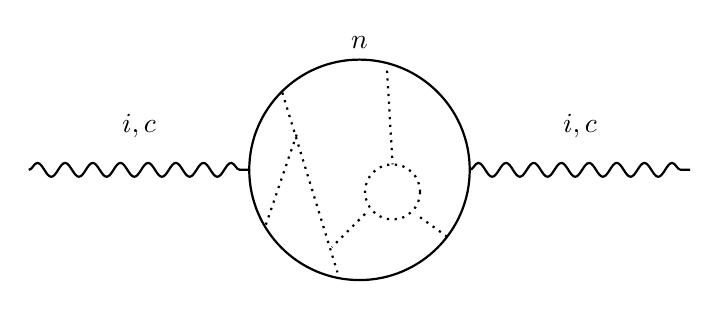
\begin{tikzpicture}[scale=1.4]
  \draw[thick,decorate, decoration={snake}] (-1,1) -- (1,1);
  \draw[thick] (2,1) circle (1) node [above=40pt] {$n$} ;
  \draw[thick,decorate, decoration={snake}] (3,1) -- (5,1);
  \draw[thick,dotted] (2.3,0.8) circle (0.25) ;
  \draw[thick,dotted] (1.3,1.7)-- (1.8,0.07);
  \draw[thick,dotted] (1.43,1.32)-- (1.15,0.5);
  \draw[thick,dotted] (2.05,0.6)-- (1.75,0.3);
  \draw[thick,dotted] (2.25,1.9)-- (2.3,1.05);
  \draw[thick,dotted] (2.55,0.57)-- (2.8,0.39);
  \node at (0,1.4) {$i,c$};
  \node at (4,1.4) {$i,c$};
\end{tikzpicture}

  \vspace{5mm}

  \caption{在规范微子传播子中引入超对称破缺的一类图. 这里的波浪线是规范超场的任意分量场; 实线是信使超场的分量场; %
  虚线是超对称破缺部分的$\,SU(3)\times SU(2)\times U(1)\,$中性超场的分量场.}%
  \label{fig:28.5}%
\end{figure}


信使超场与超对称破缺部分的其它手征和(或)规范超场以及$\,SU(3)\times SU(2)\times U(1)\,$规范超场的相互作用预期会在$\,SU(3)\times SU(2)\times U(1)\,$规范超场的分量场的传播子中产生超对称破缺. 到$\,SU(3)\times SU(2)\times U(1)\,$耦合的最低阶, 对传播子的领头阶贡献来自于图\,\ref{fig:28.5}\,中的图, 在这个图中, 一对规范线, 规范微子线或辅助$\,D\,$-场线被连到了信使场的圈上, 而这个圈又可以有任意多个与超对称破缺部分的$\,SU(3)\times SU(2)\times U(1)\,$中性场的相互作用. 因此对规范超场传播子的超对称破缺修正$\,\Delta_{ic}\,$(其中对$\,SU(3)$, $SU(2)\,$和$\,U(1)$, $i=1,2,3$, 而$\,c=V,\lambda,D\,$标记每个规范超场的不同分量)有如下的形式
\begin{align}
    \Delta_{3c}(q) &= (g_{s}^{2}/16\uppi^{2})\sum_{n} T_{3n}\Pi_{cn}(q) \:, \nonumber \\
    \Delta_{2c}(q) &= (g^{2}/16\uppi^{2})\sum_{n} T_{2n}\Pi_{cn}(q) \:, \label{28.6.1} \\
    \Delta_{1c}(q) &= (g^{\prime2}/16\uppi^{2})\sum_{n} T_{1n}\Pi_{cn}(q) \:, \nonumber
\end{align}
其中$\,n\,$标记不同的信使超场; $\Pi_{cn}(q)\,$是\,4\,-动量$\,q\,$多少有些复杂的函数; %
$T_{3n}\,$和$\,T_{2n}\,$分别是$\,SU(3)\,$和\\$\,SU(2)\,$任何生成元平方在第$\,n\,$个信使超场构成的表示中的迹(归一化成在定义表示中有$\,T_{3}=T_{2}=1/2$); 而$\,T_{1n}\,$是第$\,n\,$个信使超场的电弱超荷(hypercharge)的平方和. 一个立即的结果是规范微子获得相同形式的质量:\footnote{回忆, $B\,$微子是出现在标准模型拉格朗日量中的$\,U(1)\,$规范场的超对称伴. 我们还没有把$\,SU(2)\times U(1)\,$破缺考虑在内, 所以这里计算的规范微子, 标量夸克以及标量轻子的质量应该被理解成标准模型的$\,SU(3)\times SU(2)\times U(1)\,$-不变有效拉格朗日量中出现的参量.}
\begin{align}
    m_{\text{gluino}} &= (g_{s}^{2}/16\uppi^{2})\sum_{n} T_{3n} M_{gn} \:, \nonumber \\
    m_{\text{wino}} &= (g^{2}/16\uppi^{2})\sum_{n} T_{2n} M_{gn} \:, \label{28.6.2} \\
    m_{\text{bino}} &= (g^{\prime2}/16\uppi^{2})\sum_{n} T_{1n} M_{gn} \:, \nonumber
\end{align}
其中$\,M_{gn}\,$是表征不同信使超场的质量. 正如之前提及的, 为了保证耦合在很高的能量处统一, 我们假定$\,T_{n}\,$的和对已观测到的夸克和轻子有相同的比值:
\begin{equation}
    \sum_{n}T_{3n} =\sum_{n}T_{2n} =\sum_{n}3T_{1n}/5\equiv T \:. \label{28.6.3}
\end{equation}

超对称性在这些传播子中的破缺通过图\,\ref{fig:28.6}\,中所示的图与超对称标准模型中的标量夸克和标量轻子交互, 在这样的图中, %
一个$\,SU(3)\times SU(2)\times U(1)\,$规范玻色子或规范微子或辅助$\,D\,$场被标量夸克或标量轻子发射并再吸收. 我们要计算的低能理论还没有把$\,SU(3)\times SU(2)\times U(1)\,$考虑在内, 所以$\,SU(3)$, $SU(2)\,$和$\,U(1)\,$传播子之间没有混合, 并且每个传播子在规范指标的上的作用就像一个单位矩阵. 因此, 任何标量夸克和标量轻子被赋予的质量平方将正比于所有$\,SU(3)\times SU(2)\times U(1)\,$生成元(包含耦合常数)在那个标量夸克或标量轻子构建的表示中的平方和. $SU(2)\,$和$\,SU(3)$ 生成元在定义表示中的平方和是
\[
\sum_{a=1}^{3}\Bigl(g\sigma_{a}/2\Bigr)^{2}=\frac{3g^{2}}{4}\cdot 1 \:, \qquad
\sum_{\alpha=1}^{8}\Bigl(g_{s}\lambda_{\alpha}/2\Bigr)^{2}=\frac{4g_{s}^{2}}{3}\cdot 1 \:,
\]
其中$\,\sigma_{a}\,$是\,Pauli\,同位旋矩阵(\textcolor{foo}{5.4.18})而$\,\lambda_{a}\,$是\,Gell-Mann\,矩阵%
(\textcolor{foo}{19.7.2}). 对于$\,U(1)$, 生成元就是包含一个因子$\,g^{\prime}\,$在内的弱超荷%
(hypercharge)(\textcolor{foo}{21.3.7}). 标量夸克和标量轻子的质量平方因此有如下的形式
\begin{align}
    M_{Q}^{2}&=2\sum_{n}M_{sn}^{2}\Biggl[\frac{4}{3}\biggl(\frac{g_{s}^{2}}{16\uppi^{2}}\biggr)^{2}T_{3n}
    +\frac{3}{4}\biggl(\frac{g^{2}}{16\uppi^{2}}\biggr)^{2}T_{2n}
    +\Bigl(\frac{1}{6}\Bigr)^{2}\biggl(\frac{g^{\prime2}}{16\uppi^{2}}\biggr)^{2}T_{1n}\Biggr]\:, \nonumber \\
    M_{\bar{U}}^{2}&=2\sum_{n}M_{sn}^{2}\Biggl[\frac{4}{3}\biggl(\frac{g_{s}^{2}}{16\uppi^{2}}\biggr)^{2}T_{3n}
    +\Bigl(\frac{2}{3}\Bigr)^{2}\biggl(\frac{g^{\prime2}}{16\uppi^{2}}\biggr)^{2}T_{1n}\Biggr]\:, \nonumber \\
    M_{\bar{D}}^{2}&=2\sum_{n}M_{sn}^{2}\Biggl[\frac{4}{3}\biggl(\frac{g_{s}^{2}}{16\uppi^{2}}\biggr)^{2}T_{3n}
    +\Bigl(-\frac{1}{3}\Bigr)^{2}\biggl(\frac{g^{\prime2}}{16\uppi^{2}}\biggr)^{2}T_{1n}\Biggr]\:, \label{28.6.4} \\
    M_{L}^{2}&=2\sum_{n}M_{sn}^{2}\Biggl[\frac{3}{4}\biggl(\frac{g^{2}}{16\uppi^{2}}\biggr)^{2}T_{2n}
    +\Bigl(\frac{1}{2}\Bigr)^{2}\biggl(\frac{g^{\prime2}}{16\uppi^{2}}\biggr)^{2}T_{1n}\Biggr]\:, \nonumber \\
    M_{\bar{E}}^{2}&=2\sum_{n}M_{sn}^{2}\biggl(\frac{g^{\prime2}}{16\uppi^{2}}\biggr)^{2}T_{1n}\:, \nonumber
\end{align}
其中$\,Q$, $\bar{U}$, $\bar{D}$, $L\,$和$\,\bar{E}\,$是左手夸克双重态, 电荷为$\,-2e/3\,$和$\,+e/3\,$的左手反夸克, 左手轻子双重态以及左手带电反轻子的标量超对称伴, 而$\,M_{sn}\,$是一些用来表征第\,n\,个信使超场的新质量. %
(从$\,M_{sn}^{2}\,$中抽出因子\,2\,是为了将来的方便.) 以这种方式产生的标量夸克和标量轻子质量在所有三代中将是自动相等的, 因此避免了\,\ref{sec:28.4}\,节讨论的味改变过程伴随的问题.

我们期待所有$\,M_{gn}\,$和$\,M_{sn}\,$在量级上粗略相同, 进而使得胶微子和标量夸克有可比拟的质量, 而$\,W\,$微子, $B\,$微子和标量轻子则要轻得多, 它们的质量被电弱耦合常数压低了.

\begin{figure}[t]
  \centering
  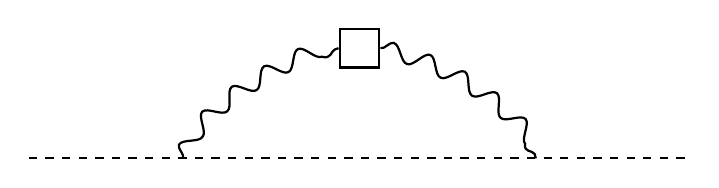
\begin{tikzpicture}[scale=1.4]

  \draw[thick, dashed] (-1,1)--(5,1);
  %\draw[thick,dashed] (3.6,1)--(5,1);
  %\draw[thick] (0.4,1)--(3.6,1);
  \node at (2,2) [rectangle, draw,thick,minimum size=14] {};
  \draw[thick,decorate, decoration={snake,amplitude=3pt,segment length=13.5pt}] (0.4,1) .. controls (0.5,1.3) and (1,1.7) .. (1.81,2);
  \draw[thick,decorate, decoration={snake,amplitude=3pt,segment length=13.5pt}] (2.19,2) .. controls (3,1.8) and (3.5,1.25) .. (3.6,1);
  %\draw[thick] (0.4,1) .. controls (0.5,1.4) and (1,1.8) .. (1.81,2);
  %\draw[thick] (2.19,2) .. controls (3,1.8) and (3.5,1.4) .. (3.6,1);

\end{tikzpicture}

  \vspace{7mm}

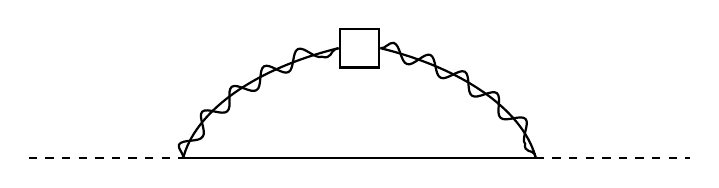
\begin{tikzpicture}[scale=1.4]

\draw[thick, dashed] (-1,1)--(0.4,1);
\draw[thick,dashed] (3.6,1)--(5,1);
\draw[thick] (0.4,1)--(3.6,1);
\node at (2,2) [rectangle, draw,thick,minimum size=14] {};
\draw[thick,decorate, decoration={snake,amplitude=3pt,segment length=13.5pt}] (0.4,1) .. controls (0.5,1.3) and (1,1.7) .. (1.81,2);
\draw[thick,decorate, decoration={snake,amplitude=3pt,segment length=13.5pt}] (2.19,2) .. controls (3,1.8) and (3.5,1.25) .. (3.6,1);
\draw[thick] (0.4,1) .. controls (0.5,1.4) and (1,1.8) .. (1.81,2);
\draw[thick] (2.19,2) .. controls (3,1.8) and (3.5,1.4) .. (3.6,1);

\end{tikzpicture}

  \vspace{5mm}

  \caption{将超对称破缺传递至标量夸克和标量轻子的图. 这里的虚线是标量夸克或标量轻子; %
  波浪线是$\,SU(3)\times SU(2) \times U(1)\,$规范玻色子或辅助$\,D\,$ 场; 实线是夸克或轻子; %
  实线和波浪线的组合线是$\,SU(3)\times SU(2)\times U(1)\,$规范微子; 而方框代表插入图\,\ref{fig:28.5}\,中所示的超对称破缺传播子修正.}
  \label{fig:28.6}%
\end{figure}

在一些合理的动力学假定下, 我们可以更进一步. 假定超对称性破缺在信使超场上的效应可以通过将这些超场以及一组$\,SU(3)\times SU(2)\times U(1)\,$-中性手征超场$\,S_{n}\,$(不一定全不相同)并进超势
\begin{equation}
    f(\Phi,\bar{\Phi},S)=\sum_{n}\lambda_{n}S_{n}\,\Phi_{n}\bar{\Phi}_{n}  \label{28.6.5}
\end{equation}
来模型化, 其中$\,\bar{\Phi}_{n}\,$和$\,\Phi_{n}\,$是$\,SU(3)\times SU(2)\times U(1)\,$复共轭表示下的左手征超场, 而$\,\lambda_{n}\,$是一组耦合常数. (这里以及后面我们将隐去在计算$\,\Phi_{n}\bar{\Phi}_{n}\,$这样的标量积时要求和的$\,SU(3)\times SU(2)\,$指标.) 对超场$\,S_{n}\,$的标量分量和辅助分量, 预期分别会有不为零的真空期望值$\,\mathscr{S}_{n}\,$和%
$\,\mathscr{F}_{n}$. 在这些模型中, 正是$\,\mathscr{F}_{n}\,$的非零值引入了$\,\Phi_{n}\,$和$\,\bar{\Phi}_{n}\,$粒子质量中的超对称破缺. \ref{sec:26.4}\,节证明了, 当规范耦合被忽略时, $\Phi_{n}\,$(和$\,\bar{\Phi}_{n}\,$)的旋量分量的质量平方是矩阵$\,\mathscr{M}_{n}^{\dag}\mathscr{M}_{n}\,$的本征值, 其中$\,\mathscr{M}_{n}\,$由方程(\ref{26.4.11})定义, 它给出
\[
\mathscr{M}_{n} =
\begin{pmatrix}
0 & \lambda_{n}\mathscr{S}_{n} \\ \lambda_{n}\mathscr{S}_{n} & 0
\end{pmatrix} \:,
\]
使得信使费米子有质量$\,\lvert\lambda_{n}\mathscr{S}_{n}\rvert$. 为了找到超场$\,\Phi_{n}\,$和$\,\bar{\Phi}_{n}\,$的标量分量%
$\,\phi_{n}\,$和$\,\bar{\phi}_{n}\,$的质量项, 我们注意到积掉$\,\Phi_{n}\,$和$\,\bar{\Phi}_{n}\,$的辅助场后给出一个势
\[
\sum_{n}\Biggl\lvert \frac{\partial f(\phi,\bar{\phi},\mathscr{S})}{\partial\phi_{n}}\Biggr\rvert^{2}
+\sum_{n}\Biggl\lvert \frac{\partial f(\phi,\bar{\phi},\mathscr{S})}{\partial\bar{\phi}_{n}}\Biggr\rvert^{2}
=\sum_{n}\lvert \lambda_{n}\mathscr{S}_{n}\rvert^{2}
\Bigl[\lvert\phi_{n}\rvert^{2}+\lvert\bar{\phi}_{n}\rvert^{2}\Bigr] \:,
\]
我们现在必须给这个势加上$\,S_{n}\,$的辅助分量的贡献, 由方程(\ref{26.4.4})的第二项给出:
\[
2\operatorname{Re}\sum_{n}\Biggl[\lambda_{n}\mathscr{F}_{n}\frac{\partial f(\phi,\bar{\phi},\mathscr{S})}{\partial\mathscr{S}_{n}}\Biggr]
=2\operatorname{Re} \sum_{n}\Bigl[\mathscr{F}_{n}\lambda_{n}\phi_{n}\bar{\phi}_{n}\Bigr] \:.
\]
这样, 有确定质量的复标量场就是$\,(\phi_{n}\pm\me^{-\mi\alpha_{n}}\bar{\phi}_{n})/\sqrt{2}$, 其中$\,\alpha_{n}\,$是%
$\lambda_{n}\mathscr{F}_{n}\,$的相位, 它们的质量平方是$\,\lvert\lambda_{n}\mathscr{F}_{n}\rvert^{2}\pm\lvert\lambda_{n}\mathscr{F}_{n}\rvert$. (注意到这种一对复标量的质量平方以一个\,Majorana\,费米子的质量平方为中心等间隔排布正是我们从求和规则(\ref{27.5.11})中所期待的.) 既然这些质量平方必须是正的, 由此得出
\begin{equation}
    \lvert\mathscr{F}_{n}\rvert \leq \lvert\lambda_{n}\rvert \lvert \mathscr{S}_{n}\rvert^{2}\:. \label{28.6.6}
\end{equation}


模型中基于方程(\ref{28.6.5})的胶微子质量由图\,\ref{fig:28.5}\,中所示的那种图给出, 只不过现在只有一个圈, %
不包含图\,\ref{fig:28.5}\,中的虚线表示的部分. 一个细致的计算给出方程(\ref{28.6.2})中的系数$\,M_{gn}\,$是\cite{31}
\begin{equation}
    M_{gn} = \frac{\lvert \mathscr{F}_{n}\rvert}{\lvert\mathscr{S}_{n}\rvert}\,g\,
    \biggl(\frac{\lvert \mathscr{F}_{n}\rvert}{\lvert\lambda_{n}\rvert\lvert\mathscr{S}_{n}\rvert^{2}}\biggr)\:,
    \label{28.6.7}
\end{equation}
其中
\begin{align}
    g(x) &= \frac{1}{2x^{2}} \Bigl[(1+x)\ln(1+x)+(1-x)\ln(1-x)\Bigr] \nonumber \\
    &= 1 + \frac{x^{2}}{6} + \frac{x^{4}}{15} + \frac{x^{6}}{28} + \cdots \:. \label{28.6.8}
\end{align}
标量夸克和标量轻子的质量由图\,\ref{fig:28.6}\,中的图给出, 它现在只包含两个圈. %
另一个细致的计算给出方程(\ref{28.6.4})中的质量参量$\,M_{sn}^{2}\,$是\cite{31}
\begin{equation}
    M_{sn}^{2}=\frac{\lvert \mathscr{F}_{n}\rvert^{2}}{\lvert\mathscr{S}_{n}\rvert^{2}}\,
    f\biggl(\frac{\lvert \mathscr{F}_{n}\rvert}{\lvert\lambda_{n}\rvert\lvert\mathscr{S}_{n}\rvert^{2}}\biggr)
    \:, \label{28.6.9}
\end{equation}
其中
\begin{align}
    f(x) &= \frac{1+x}{x^{2}}\,\biggl[\ln(1+x)-2\operatorname{Li}_{2}\biggl(\frac{x}{1+x}\biggr)
    +\frac{1}{2}\operatorname{Li}_{2}\biggl(\frac{2x}{1+x}\biggr) \biggr] + x\to -x  \nonumber \\
    &= 1+ \frac{1}{36}x^{2}-\frac{11}{450}x^{4}-\frac{319}{11760}x^{6}+\cdots, \label{28.6.10}
\end{align}
而$\,\operatorname{Li}_{2}\,$是二重对数
\begin{equation}
    \operatorname{Li}_{2}(x) \equiv - \int_{0}^{x} \frac{\ln(1-t)}{t}\,\dif t\:. \label{28.6.11}
\end{equation}
特别地, 如果(也是通常假定的)各个$\,S_{n}\,$的值都相同, 并且如果对所有$\,n\,$有$\,\lvert\mathscr{F}\rvert\ll\lvert\lambda_{n}\rvert\lvert\mathscr{S}\rvert^{2}$, 那么方程(\ref{28.6.9})和(\ref{28.6.7})中的$\,f\,$和$\,g\,$可以被设为\,1, 使得
\begin{equation}
    M_{gn}=M_{sn}=\lvert \mathscr{F}\rvert / \lvert \mathscr{S} \rvert \equiv M \:. \label{28.6.12}
\end{equation}
利用方程(\ref{28.6.3}), 我们可以把规范微子质量(\ref{28.6.2})表示成
\begin{align}
    & m_{\text{wino}}= (g^{2}/16\uppi^{2}) TM \:, \nonumber \\
    & m_{\text{bino}}= (5/3)(g^{\prime2}/16\uppi^{2})TM \:, \label{28.6.13} \\
    & m_{\text{gluino}} = (g_{s}^{2}/16\uppi^{2})TM \:, \nonumber
\end{align}
标量夸克和标量轻子的质量平方(\ref{28.6.4})则变成
\begin{align}
    M_{Q}^{2}&=2TM^{2}\Biggl[\frac{4}{3}\biggl(\frac{g_{s}^{2}}{16\uppi^{2}}\biggr)^{2}
    +\frac{3}{4}\biggl(\frac{g^{2}}{16\uppi^{2}}\biggr)^{2}
    +\frac{5}{3}\Bigl(\frac{1}{6}\Bigr)^{2}\biggl(\frac{g^{\prime2}}{16\uppi^{2}}\biggr)^{2}\Biggr]\:, \nonumber \\
    M_{\bar{U}}^{2}&=2TM^{2}\Biggl[\frac{4}{3}\biggl(\frac{g_{s}^{2}}{16\uppi^{2}}\biggr)^{2}
    +\frac{5}{3}\Bigl(\frac{2}{3}\Bigr)^{2}\biggl(\frac{g^{\prime2}}{16\uppi^{2}}\biggr)^{2}\Biggr]\:, \nonumber \\
    M_{\bar{D}}^{2}&=2TM^{2}\Biggl[\frac{4}{3}\biggl(\frac{g_{s}^{2}}{16\uppi^{2}}\biggr)^{2}
    +\frac{5}{3}\Bigl(-\frac{1}{3}\Bigr)^{2}\biggl(\frac{g^{\prime2}}{16\uppi^{2}}\biggr)^{2}\Biggr]\:, \label{28.6.14} \\
    M_{L}^{2}&=2TM^{2}\Biggl[\frac{3}{4}\biggl(\frac{g^{2}}{16\uppi^{2}}\biggr)^{2}
    +\frac{5}{3}\Bigl(\frac{1}{2}\Bigr)^{2}\biggl(\frac{g^{\prime2}}{16\uppi^{2}}\biggr)^{2}\Biggr]\:, \nonumber \\
    M_{\bar{E}}^{2}&=2TM^{2}\frac{5}{3}\biggl(\frac{g^{\prime2}}{16\uppi^{2}}\biggr)^{2}\:, \nonumber
\end{align}
没有什么特别的理由期待会有$\,\lvert\mathscr{F}\rvert\ll\lvert \lambda_{n}\mathscr{S}\rvert^{2}$, 但这个假定的限制性实际上不是很强, 这是因为方程(\ref{28.6.6})已经要求$\,\lvert\mathscr{F}\rvert\leq\lvert\lambda_{n}\rvert\lvert\mathscr{S}\rvert^{2}$, 而除非$\,x\,$非常接近于\,1, 否则函数$\,f(x)\,$和$\,g(x)\,$在$\,x<1\,$时与\,1\,相差不大.

通过使用\,\ref{sec:27.6}\,节描述过的\,Seiberg\,的全纯讨论,\cite{33} Giudice\,和\,Rattazzi\cite{32}解释了结果(\ref{28.6.13}) 和(\ref{28.6.14})为何如此简单. 假如我们对信使超场引入像(\ref{28.6.5})这样的超势, 但只有一个外单态超场$\,S$:
\begin{equation}
    f(S,\Phi)=S\sum_{n}\lambda_{n}\,\Phi_{n}\bar{\Phi}_{n} \:. \label{28.6.15}
\end{equation}
此外, 对于在重整化标度$\,\mu\,$处的威尔逊型有效拉格朗日量, 其中的规范超场$\,V_{i}\,$(对于$\,SU(3)$, $SU(2)$ 和$\,U(1)$, $i=3,2,1$)的动能项现在将采取形式
\begin{equation}
    \mathscr{L}_{\text{gauge},\mu}=\operatorname{Re}
    \Biggl[\sum_{i}N_{i}(S,\mu)\sum_{\alpha\beta}(W_{iL\alpha}\epsilon_{\alpha\beta}W_{iL\beta})\Biggr]_{\mathscr{F}}\:,
    \label{28.6.16}
\end{equation}
其中一些函数$\,N_{i}(S,\mu)\,$被替换成了方程(\ref{27.3.22})中的因子$\,1/2g_{i}^{2}(\mu)$. (这里扔掉了$\,\theta\,$-项是因为它在微扰论中没有任何效应. 对$\,W_{iL\alpha}\,$上标记$\,SU(3)\,$和$\,SU(2)\,$伴随表示不同成员的指标暗含了一个求和, 这里没有显式地写出.) 规范耦合常数现在通过令超场$\,S\,$等于它的标量分量的真空期望值$\,\mathscr{S}\,$给出
\begin{equation}
    \frac{1}{2g_{i}^{2}(\mu)} = N_{i}(\mathscr{S},\mu) \:. \label{28.6.17}
\end{equation}
另外, 回忆起$\,W_{iL\alpha}=\lambda_{iL\alpha}+O(\theta)\,$并使用方程(\ref{27.2.11}), 拉格朗日密度(\ref{28.6.16})中规范微子场的二阶项在相差一些导数项的意义下是
\[
-2\sum_{i}\operatorname{Re}\Bigl[N_{i}(\mathscr{S},\mu)
\Bigl(\bar{\lambda}_{iR}\,\slashed{\partial}\lambda_{iR}\Bigr)
+[N_{i}(S,\mu)]_{\mathscr{F}}\Bigl(\lambda_{iL}^{\mathrm{T}}\epsilon\lambda_{iL}\Bigr)\Bigr] \:.
\]
这给出了规范微子质量
\begin{equation}
    m_{gi}(\mu) = \biggl\lvert \frac{[N_{i}(s,\mu)]_{\mathscr{F}}}{2N_{i}(\mathscr{S},\mu)}\biggr\rvert
    = g^{2}_{i}(\mu) \Bigl\lvert [N_{i}(S,\mu)]_{\mathscr{F}} \Bigr\rvert \:. \label{28.6.18}
\end{equation}
现在我们来考虑$\,N_{i}(\mathscr{S},\mu)\,$作为正实$\,\mathscr{S}\,$的函数的行为, 其中信使超场的相位都被调整成是的所有 $\lambda_{n}\,$都是正实的. 假定我们在所有信使粒子质量之上的某个标度$\,\mu=K\,$处固定规范耦合的值$\,g_{i}(\mu)$. 将重整化群方程$\,\mu\dif g_{i}/\dif\mu=b_{i}g_{i}^{3}\,$中的常数$\,b_{i}\,$在$\,\mu\,$穿过不同信使质量时发生的变化考虑在内, %
当$\,\mu$ {\kai{低于}}低于所有信使粒子的质量时, 这个方程有如下形式的解
\[
    \frac{1}{g_{i}^{2}(\mu)} =\frac{1}{g_{i}^{2}(K)} - 2b_{i}^{(0)}\ln\biggl(\frac{M_{1}}{K}\biggr)
    - 2b_{i}^{(1)}\ln\biggl(\frac{M_{2}}{M_{1}}\biggr) - \cdots
    - 2b_{i}^{(N)}\ln\biggl(\frac{M_{N}}{\mu}\biggr) \:,
\]
其中我们标记信使粒子使得它们的质量$\,M_{n}=\lambda_{n}\mathscr{S}\,$满足
\[
M_{1}>M_{2}>\cdots> M_{N} \:,
\]
而在计算$\,b_{i}^{(n)}\,$时则只考虑质量小于$\,M_{n}\,$的粒子. 由于所有$\,M_{n}\,$都正比于$\,\mathscr{S}$, %
我们看到$\,N_{i}(\mathscr{S},\mu)\,$对 $\mathscr{S}\,$的依赖是
\begin{equation}
    N_{i}(\mathscr{S},\mu) = -b_{i}^{\text{messenger}} \ln\mathscr{S}+\mathscr{S}\text{-无关项} \:,\label{28.6.19}
\end{equation}
其中$b_{i}^{\text{messenger}}=b_{i}^{(0)}-b_{i}^{(N)}\,$是所有信使超场对$\,b_{i}\,$的贡献. %
根据方程(\ref{27.9.45})(其中$\,C_{i1}=0\,$且$\,C_{i2}^{f}=C_{i2}^{s}=\sum_{n}T_{in}$), 这是
\begin{equation}
    b_{i}^{\text{messenger}}=\frac{1}{16\uppi^{2}}\sum_{n}T_{in} \:. \label{28.6.20}
\end{equation}
由于超对称性要求$\,N_{i}(S,\mu)\,$是$\,S\,$的全纯函数, 我们看到
\begin{equation}
    N_{i}(\mathscr{S},\mu) = -\frac{1}{16\uppi^{2}}\sum_{n}T_{in}\ln S+S\text{-无关项}\:.\label{28.6.21}
\end{equation}
在$\,S=\mathscr{S}\,$附近展开, 到$\,\mathscr{F}\,$的一阶, 我们有$\,[\ln\mathscr{S}]_{\mathscr{F}}=\mathscr{F}/\mathscr{S}$, 这样方程(\ref{28.6.18})给出规范微子质量
\begin{equation}
    m_{gi}(\mu)=\frac{g_{i}^{2}(\mu)}{16\uppi^{2}}\sum_{n}T_{in}\,\biggl\lvert\frac{\mathscr{F}}{\mathscr{S}}\biggr\rvert\:. \label{28.6.22}
\end{equation}
利用方程(\ref{28.6.3}), 我们看到这与我们前面的结果(\ref{28.6.13})相同. 代替规范超场, Giudice\,和\,Rattazzi\,\\ 通过类似的方法研究夸克和轻子超场的动量项获得了标量夸克和标量轻子的方程(\ref{28.6.14}).

附带地, 如果我们假定超对称破缺部分在某个以已知夸克和轻子以及信使场作为完整表示的大统一群$\,G\,$下是不变的, %
不做像方程(\ref{28.6.5})这样的特殊动力学假定也可获得方程(\ref{28.6.13})和 (\ref{28.6.14})(一般情况下, %
方程(\ref{28.6.13})和(\ref{28.6.14})中的$\,M\,$值不同). 在这一情况下, 方程(\ref{28.6.2})和 (\ref{28.6.4})中的%
系数$\,M_{gn}\,$和$\,M_{sn}\,$将分别有值$\,M_{g}(d)\,$和$\,M_{s}(d)$, 它们仅依赖于第$\,n\,$个信使场所属的$\,G\,$的%
不可约表示$\,d$. 对属于$\,G\,$的任何不可约表示$\,d\,$的$\,n$, $T_{in}\,$对其求和与方程(\ref{28.6.3})中的和有相同的比值, %
所以$\,\sum_{n\in d} T_{in}=k_{i}T(d)$, 其中$\,k_{3}=k_{2}=1$, $k_{1}=5/3$, 因此
\[
\sum_{n}T_{in}M_{gn}=\sum_{d}M_{g}(d)\sum_{n\in d}T_{in} = k_{i}M_{g} \:,
\]
其中$\,M_{g}=\sum_{d}M_{g}(d)T(d)$. 同样的,
\[
\sum_{n}T_{in}M_{sn}^{2} =\sum_{d}M_{s}^{2}(d)\sum_{n\in d}T_{in} = k_{i}M_{s}^{2} \:,
\]
其中$\,M_{s}^{2}=\sum_{d}M_{s}^{2}(d)T(d)$. 这样, 除了$\,TM\,$要被换成$\,M_{g}\,$以及$\,2TM^{2}\,$要被换成$\,M_{s}^{2}$, %
方程(\ref{28.6.2})和\\(\ref{28.6.4})将会给出方程(\ref{28.6.13})和(\ref{28.6.14}). 然而, 如果信使的质量标度远低于大统一的标度, $M_{gn}$ 和$\,M_{sn}\,$遵循$\,G\,$下的不变性这个假定是不合道理的, 这是因为, 无论我们假定大统一群是什么, %
对于像$\,\lambda_{n}\,$这样的耦合常数, 如果同属大统一群同一表示的$\,\Phi_{n}\,$有不相同的%
$\,SU(3)\times SU(2)\times U(1)\,$的量子数, 那么$SU(3)\times SU(2)\times U(1)\,$规范相互作用会使得这些耦合常数的跑动不相同.

这些结果要做各种辐射修正, 其中最重要的一个是我们必须使用$\,g_{s}$, $g\,$和$\,g^{\prime}\,$在与要计算的质量可比拟的标度重整化的值. 诚然, 方程(\ref{28.6.13})中给出的规范微子的质量比值也可以从完全不同的假定中推导出来: 所有规范微子的质量在耦合常数之间的关系是$\,g_{s}^{2}=g^{2}=5g^{\prime2}/3\,$的大统一标度处相等, 并且就像重整化方程描述的那样在低能标处变得不同.

数值结果的一个例子是, 假定信使超场构成电荷为$\,e/3\,$的$\,SU(2)\,$单态$\,SU(3)\,$三重态以及电荷为$\,0\,$和$\,-e\,$的%
$\,SU(2)\,$双重态$\,SU(3)\,$单态, 以及处在$\,SU(3)\times SU(2)\times U(1)\,$复共轭表示下的左手征超场. 那么正如前面提及的, %
方程(\ref{28.6.3})满足于$\,T=2\times 1/2=1$, 所以通过使用规范耦合的正确值, 计算可得标量夸克, 胶微子, $L\,$标量轻子, $W\,$微子, $E\,$标量轻子以及$\,B\,$微子的质量比值是\cite{34}$11.6::7.0::2.5::2::1.1::1.0$.

除了耦合常数跑动, 还有额外的修正. 根据一个计算,\cite{34} 在有一个电荷为$\,e/3\,$的$\,SU(2)\,$单态 $SU(3)\,$三重态以及%
电荷为$\,0\,$和$\,-e\,$的$\,SU(2)\,$双重态$\,SU(3)\,$单态, 以及处在$\,SU(3)\times SU(2)\times U(1)\,$复共轭表示下的左手征超场的模型中, 辐射修正给出的标量夸克, 胶微子, $L\,$标量轻子, $W\,$微子, %
$E\,$标量轻子以及$\,B\,$微子的质量比值是$\,9.3::6.4::2.6::1.9::1.35::1.0$.

正如我们在上一节看到的, $W\,$微子和$\,B\,$微子可以与带荷以及中性希格斯微子混合, 所以这里计算出的$\,W\,$微子和$\,B\,$微子质量必须视为计算称为{\kai{带荷微子}}和{\kai{中性微子}}的混合物的物理质量的输入量, 而不是物理质量本身.

现在我们来考虑这些模型中\,Higgs\,标量的质量. 如果我们仅考虑这些标量通过与超对称破缺部分的规范相互作用的两圈图获得质量, 那么由于它们与左手轻子双重态(除符号外)有相同的 $SU(3)\times SU(2)\times U(1)\,$量子数, 它们的质量将由像方程组(\ref{28.6.4})中的第四个方程那样的公式给出
\begin{align}
    [m_{1}^{2}]_{\text{2 loop}} &= [m_{2}^{2}]_{\text{2 loop}} = M_{L}^{2} \nonumber \\
    &=\sum_{n}M_{sn}^{2}\Biggl[\frac{3}{4} \biggl(\frac{g^{2}}{16\uppi^{2}}\biggr)^{2} T_{2n}
    +\Bigl(\frac{1}{2}\Bigr)^{2}\biggl(\frac{g^{\prime 2}}{16\uppi^{2}}\biggr)^{2} T_{1n}\Biggr]^{2} \:. \label{28.6.23}
\end{align}
如果这就是整个故事, 那么(除非$\,\tan\beta\,$非常接近于一)就不可能达到上一节发现的$\,SU(2)\times U(1)\,$破缺条件, %
即$\,m_{1}^{2}+\lvert\mu\rvert^{2}\,$和$\,m_{2}^{2}+\lvert\mu\rvert^{2}\,$中有一个为负. 幸运的是, 顶夸克和标量夸克的大质量给了$\,m_{2}^{2}\,$一个负贡献, 这自然地导致了电弱对称性的自发破缺. Higgs\,双重态与第三代夸克超场的耦合由如下超势描述
\begin{equation}
    f_{\text{3rd gen}}= \lambda_{b}\Bigl(H_{1}^{\mathrm{T}}eQ\Bigr)\bar{B}
    +\lambda_{t} \Bigl(H_{2}^{\mathrm{T}}eQ\Bigr) \bar{T} \:, \label{28.6.24}
\end{equation}
其中$\,Q\,$是$\,SU(2)\,$夸克左手征超场双重态$\,(T,B)$, 而$\,\bar{T}\,$和$\,\bar{B}\,$是左手反顶夸克和反底夸克的左手征超场, $\lambda_{t}\,$和$\,\lambda_{b}\,$是\,Yukawa\,耦合, 与$\,t\,$夸克和$\,b\,$夸克的质量关系是$\,m_{t}=\lambda_{t}v_{2}\,$和%
$\,m_{b}=\lambda_{b}v_{1}$. 这样超势中与标量夸克和\,Higgs\,场相互作用相关的项就由方程(\ref{26.4.7})的最后一项给出
\begin{align}
    V_{sq\:H}&=\Bigl\lvert \lambda_{b}\mathscr{H}_{1}^{-}\bar{\mathscr{B}}
    +\lambda_{t}\mathscr{H}_{2}^{0}\bar{\mathscr{T}}\Bigr\rvert^{2}
    +\Bigl\lvert \lambda_{b}\mathscr{H}_{1}^{0}\bar{\mathscr{B}}
    +\lambda_{t}\mathscr{H}_{2}^{+}\bar{\mathscr{T}}\Bigr\rvert^{2} \nonumber \\
    &\quad +\lvert\lambda_{b}\rvert^{2}\Bigl\lvert \mathscr{H}_{1}^{0}\mathscr{B}-\mathscr{H}_{1}^{-}\mathscr{T}\Bigr\rvert^{2}
    +\lvert\lambda_{t}\rvert^{2}\Bigl\lvert \mathscr{H}_{2}^{+}\mathscr{B}
    -\mathscr{H}_{2}^{0}\mathscr{T}\Bigr\rvert^{2}  \:, \label{28.6.25}
\end{align}
其中下标代表超场的标量场分量. 这样标量夸克圈对$\,\mathscr{H}_{1}\,$和$\,\mathscr{H}_{2}\,$的贡献就是
\begin{equation}
    V_{H}^{\text{squark loop}} = 3\langle \mathscr{S}\mathscr{S}^{\ast}\rangle
    \Bigl[2\lvert\lambda_{b}\rvert^{2}\Bigl(\mathscr{H}_{1}^{\dag}\mathscr{H}_{1}\Bigr)
    +2\lvert\lambda_{t}\rvert^{2}\Bigl(\mathscr{H}_{2}^{\dag}\mathscr{H}_{2}\Bigr)\Bigr] \:, \label{28.6.26}
\end{equation}
其中$\,\langle\mathscr{S}\mathscr{S}^{\ast}\rangle\,$是任何一个标量夸克场与它的复共轭在同一时空点的真空期望值. (为了使上式对所有标量夸克类型都相同, 我们在这里使用了方程(\ref{28.6.4}), 它告诉我们标量夸克质量$\,M_{Q}\,$在$\,\mathscr{T}$, $\mathscr{B}$, $\bar{\mathscr{T}}\,$和$\,\bar{\mathscr{B}}\,$标量夸克之间变化不大). %
真空期望值$\,\langle\mathscr{S}\mathscr{S}^{\ast}\rangle\,$在最低阶是
\begin{equation}
    \langle \mathscr{S}\mathscr{S}^{\ast}\rangle \equiv \langle \mathscr{S}(x)\mathscr{S}^{\ast}(x)\rangle_{\text{VAC}}
    =\frac{-\mi}{(2\uppi)^{2}}\int\frac{\dif^{4}p}{p^{2}+M_{Q}^{2}-\mi\epsilon} \:. \label{28.6.27}
\end{equation}
这当然是发散的, 但如果标量夸克有夸克的零裸质量, 那么它对超对称破缺系数的贡献将被夸克圈抵消, 所以夸克圈的效应就是给(\ref{28.6.7})减去形式相同但是$\,M_{Q}\,$被替换成零的式子, 在\,Wick\,旋转后变成
\begin{align*}
    \langle \mathscr{S}\mathscr{S}^{\ast}\rangle &\to \frac{M_{Q}^{2}\,\mi}{(2\uppi)^{4}}
    \int\frac{\dif^{4}p}{(p^{2}+M_{Q}^{2}-\mi\epsilon)(p^{2}-\mi\epsilon)} \\
    &=-\frac{M_{Q}^{2}}{(2\uppi)^{4}} \int^{M^{2}}_{0}\frac{\uppi^{2}\dif p^{2}}{p^{2}+M_{Q}^{2}}
    \simeq -\frac{M_{Q}^{2}}{16\uppi^{2}}\ln \Biggl(\frac{M^{2}}{M_{Q}^{2}}\Biggr) \:.
\end{align*}
我们在信使质量$\,M\,$处插入了一个紫外截断, 因为当动量在$\,M\,$之上时, 标量夸克质量必须被换成一个动量相关的质量, 而这个质量在非常高的动量处趋于超对称值零. 在方程(\ref{28.6.26})中做这个减除给出了标量夸克圈和夸克圈对势的净贡献:
\begin{equation}
    (V_{m})^{\text{3 loop}}= \frac{3M_{Q}^{2}}{16\uppi^{2}}\ln \Biggl(\frac{M^{2}}{M_{Q}^{2}}\Biggr)\,
    \Biggl[2\lvert\lambda_{b}\rvert^{2}\Bigl(\mathscr{H}_{1}^{\dag}\mathscr{H}_{1}\Bigr)
    +2\lvert\lambda_{t}\rvert^{2}\Bigl(\mathscr{H}_{2}^{\dag}\mathscr{H}_{2}\Bigr) \Biggr]  \:. \label{28.6.28}
\end{equation}
(因为标量夸克质量由两圈图给出, 这是一个三圈贡献. 势中还有\,Higgs\,和标量夸克超场的二次项, 来源于\,Higgs\,和标量夸克项在$\,SU(2)\times U(1)\,$规范场$\,D\,$-分量平方中的乘积. 它们对\,Higgs\,质量没有三圈贡献, 这是因为标量夸克的每个$\,SU(2)\times U(1)\,$量子数之和为零, 这使得它们对$\,SU(2)\times U(1)\,$ 规范场$\,D\,$-分量的贡献有一个零期望值.) %
比较方程(\ref{28.6.28})与(\ref{28.5.9})并给质量加上两圈贡献(\ref{28.6.23}), 我们就看到
\begin{equation}
    m_{1}^{2} \simeq M_{L}^{2}-\frac{3M_{Q}^{2}\lvert\lambda_{b}\rvert^{2}}{8\uppi^{2}}
    \ln \Biggl(\frac{M^{2}}{M_{Q}^{2}}\Biggr) \:, \label{28.6.29}
\end{equation}
\begin{equation}
    m_{2}^{2} \simeq M_{L}^{2}-\frac{3M_{Q}^{2}\lvert\lambda_{t}\rvert^{2}}{8\uppi^{2}}
    \ln \Biggl(\frac{M^{2}}{M_{Q}^{2}}\Biggr) \:, \label{28.6.30}
\end{equation}
使用方程(\ref{28.6.14})以及$\,\lvert\lambda_{t}\rvert=m_{t}/v_{2}=m_{t}(2\sqrt{2}G_{F})^{1/2}/\sin\beta$, %
我们可以将方程(\ref{28.6.30})写成
\begin{align}
    m_{2}^{2} &\simeq 2TM^{2}\Biggl[\frac{3}{4}\Biggl(\frac{g^{2}}{16\uppi^{2}}\Biggr)^{2}
    +\frac{5}{12}\Biggl(\frac{g^{\prime2}}{16\uppi^{2}}\Biggr)^{2} \nonumber \\
    &\quad -\frac{\sqrt{2}G_{F}m_{t}^{2}}{\uppi^{2}\sin^{2}\beta}\Biggl(\frac{g^{2}_{s}}{16\uppi^{2}}\Biggr)^{2}
    \ln\Biggl(\frac{3}{8T(g_{s}^{2}/16\uppi^{2})}\Biggr)\Biggr]\:. \label{28.6.31}
\end{align}
对$\,T=1$, $g_{s}^{2}/4\uppi=0.118$, $g^{2}/4\uppi=0.0340$, $g^{\prime2}/4\uppi=0.0101$, 以及$\,m_{t}=180\,\mathrm{GeV}$, %
这是
\begin{equation}
    m_{2}^{2}\simeq M_{L}^{2}\Biggl[ 1-\frac{3.06}{\sin^{2}\beta}\Biggr] \:, \label{28.6.32}
\end{equation}
它对于所有$\,\beta\,$值都是负的, 因此提供了电弱规范对称性自发破缺的一个自然机制. 另外, $M_{L}^{2}=(0.91\times 10^{-4})M^{2}/8\uppi^{2}.$ 除非$\,\tan\beta\,$非常大, 我们有$\,\lvert\lambda_{b}\rvert\ll\lvert\lambda_{t}\rvert$, %
所以方程(\ref{28.6.27})给出
\begin{equation}
    m_{1}^{2}\simeq m_{L}^{2} \:. \label{28.6.33}
\end{equation}


在电弱唯象学方面, 规范传递的超对称模型给出的预测中最不确定且最不让人满意与超对称保留项%
$\,\mu[(H_{1}^{\mathrm{T}}eH_{2})]_{\mathscr{F}}\,$中的参量$\,\mu\,$以及拉格朗密度中相关的超对称破缺项$\,B\mu\,$有关.
它们相互关联是因为\,Higgs\,超场与规范超场, 轻子超场以及夸克超场的相互作用在如下的对称性下是不变的,
\begin{align}
    &H_{1}\to \me^{\mi\varphi}H_{1}\:, \qquad H_{2} \to \me^{\mi\varphi}H_{2} \:, \nonumber \\
    &Q\to \me^{-\mi\varphi}Q \:, \qquad \:\: V_{i}\to V_{i} \:, \label{28.6.34} \\
    &\bar{D}\to \bar{D} \:, \qquad \qquad \bar{U}\to\bar{U} \:, \nonumber
\end{align}
当没有超势项$\,\mu(H_{1}^{\mathrm{T}}eH_{2})\,$时, 这将阻止辐射修正在标量场势中产生%
$\,B\mu\operatorname{Re}(\mathscr{H}_{1}^{\mathrm{T}}e\mathscr{H}_{2})$.

$B\mu\,$不可能为零, 否则方程(\ref{28.5.22})和(我们看到的)$\,m_{A}\neq=0\,$将给出$\,\sin2\beta=0$, 换句话说, %
要么$\,v_{1}=0\,$要么$\,v_{2}=0$, 而这将给出要么所有带$\,-e/3\,$电荷的夸克以及带电轻子是无质量的, 要么所有带$\,+2e/3\,$电荷的夸克是无质量的. (如果$\,B\mu=0\,$且$\,\mu=0$, 那么这个问题将延续至所有阶, 这是因为$\,v_{1}\,$和$\,v_{2}\,$均有非零的真空期望值意味着在变换(\ref{28.6.34})和电弱$\,U(1)\,$规范变换的任意组合变换下的对称性将是自发破缺的, 所以$\,\mathsf{C}\,$为奇的中性标量将是$\,m_{A}=0\,$的\,Goldstone\,玻色子.) 自然想法是尝试将$\,B\mu\,$的非零期望值解释为如下理论中的辐射修正: %
变换(\ref{28.6.34})下的对称性被拉格朗日密度中的一个超对称项$\,\mu[(H_{1}^{\mathrm{T}}e H_{2})]_{\mathscr{F}}\,$明显破缺了.
这会在信使标度给$\,B\mu\,$一个非常小的值, 但是重整化群效应会在低能处极大地增强这个值. 根据方程(\ref{28.5.22}), %
一个相对小的$\,B\mu\,$与顶夸克的大质量来自于大的$\,\tan\beta\,$值这个想法很相符. 无论如何, %
带荷微子质量上的实验下界告诉我们$\,\mu\,$至少约$\,60\,\mathrm{GeV}$.

$\mu\,$的非零值引起的麻烦是它带回了超对称本要解决的等级问题: 取代为什么拉格朗日密度中的\,Higgs\,质量项为什么远小于普朗克质量或者规范耦合统一时的质量, 我们现在必须要问为什么$\,\mu\,$这么小?

如果\,Higgs\,超场与超对称破缺部分的相互作用方式使得$\,\mu[(H_{1}^{\mathrm{T}}eH_{2})]\,$被某个对称性禁止掉, 而在这个对称性自发破缺时出现, 那么等级问题就能得以解决. 如果对称性是离散而非连续的, 那么就可以避免出现无质量\,Goldstone\,玻色子. %
最简单的可能性就是扩张对称变换(\ref{28.6.34})以包含变换
\[
S\to \me^{-2\mi\varphi}S \:,
\]
这个变换将会允许超势中有如下形式的项
\[
\lambda^{\prime}S(\mathscr{H}_{1}^{\mathrm{T}}e\mathscr{H}_{2}) \:.
\]
我们可以通过在超势中再引入一个$\,S^{3}\,$项来避免连续对称性, 这使得仅在$\,\varphi\,$是$\,2\uppi/3\,$的倍数时, 拉格朗日量在变换下才是不变的, 而这足以禁止$\,\mu\,$有非零的裸值. 在这一情况下, %
$S\,$的标量分量和辅助分量的非零期望值$\,\mathscr{S}\,$和$\,\mathscr{F}\,$给出
\[
B\mu=\lvert \lambda^{\prime}\mathscr{F}\rvert \:, \qquad \mu=\lvert \lambda^{\prime}\mathscr{S}\rvert \:.
\]
这将导致$\,B\,$有一个非常大的$\,\lambda\,$-相关值$\,M$, 由方程(\ref{28.6.12})给定, %
它要比标量夸克或胶微子的质量大一个约为$\,(g_{s}^{2}/16\uppi)^{-1}\simeq 100\,$的因子. 但另一方面, %
由于方程(\ref{28.6.32})和(\ref{28.6.33})给出$\,m_{1}^{2}+m_{2}^{2}<0$, 稳定性条件(\ref{28.5.11})将要求$\,\lvert\mu\rvert \geq M/2$, 因此方程(\ref{28.5.22})将要求$\,m_{A}\,$也远大于标量夸克和标量轻子的质量. 除非$\,\tan\beta\,$非常接近于一, %
否则这被关系(\ref{28.5.23})以及$\,m_{1}^{2}\,$和$\,m_{2}^{2}\,$的估计值(\ref{28.6.33})和 (\ref{28.6.32})排除了.

我们会在\,\ref{sec:31.6}\,节看到, 引力传递的超对称破缺理论自然地给出了可接受的$\,B\mu\,$值和$\,\mu\,$值. 这种理论由一个非常高的超对称破缺能标表征, 在各个版本中不是$\,10^{11}\,\mathrm{GeV}\,$就是$\,10^{13}\,\mathrm{GeV}$. 有数个方案\cite{35}谋求在超对称性在相对低的能量处破缺的理论中获得可接受的$\,B\mu\,$和$\,\mu\,$值, 例如规范传递的超对称破缺理论, 但没有一个特别引人注目. 另外, 由于我们不知道$\,\mu\,$来自哪里, 我们没有任何理由认为它是实的, %
所以规范传递超对称破缺的理论有着产生太多$\,\mathsf{CP}\,$破坏的风险, 和$\,\ref{sec:28.4}\,$节更一般框架中的情况一样.

同标量质量平方$\,m_{1}^{2}\,$和$\,m_{2}^{2}\,$一样, 方程(\ref{28.4.1})中的参量$\,A_{ij}\,$和$\,C_{ij}\,$由两圈图给出. 然而它们的量纲是质量而非质量平方, 并且它们远小于标量和规范微子的质量, 所以它们对超对称破缺的贡献相对而言就不那么重要.

就像任何超对称在能量远低于$\,10^{10}\,\mathrm{GeV}\,$处破缺的模型一样, 在所有基于规范传递超对称破缺的模型中, %
$R\,$为奇的最轻粒子是引力微子. 而我们将在\,\ref{sec:31.3}\,节看到, 引力微子质量的量级是$\,\sqrt{G}\,$乘以表征超对称破缺的能量平方$\,F$, %
$F\,$的定义使得真空能是$\,F^{2}/2$. 当超对称是被$\,SU(3)\times SU(2)\times U(1)\,$-中性手征超场$\,S_{n}\,$的%
$\,\mathscr{F}\,$-项$\,\mathscr{F}_{n0}\,$破缺时, 我们有$\,F^{2}=\sum_{n}\lvert\mathscr{F}_{n0}\rvert^{2}$. %
如果$\,S_{n}\,$的拉格朗日量中没有大的无量纲参量, 那么这一模型中的标量夸克质量是$\,g_{s}^{2}\sqrt{F}/16\uppi^{2}\approx10^{-2}\sqrt{F}\,$阶的, %
所以为了使其小于自然性给出的上界$\,10^{4}\,\mathrm{GeV}$, 我们必须有$\,\sqrt{F}<10^{6}\,\mathrm{GeV}$, 这给出的引力微子质量小于$\,1\,\mathrm{keV}$. %
引力耦合在可达到能标处是如此的弱以至于真正能够产生的是引力微子螺旋度为$\,\pm1/2$ 的态, 而这些态的行为就像戈德斯通微子态. %
正如方程(\ref{27.5.12})表明的, 在这里讨论的模型中, 戈德斯通微子场伴随着系数$\,\mi\sqrt{2}\mathscr{F}_{n}\,$出现在$\,S_{n}\,$的费米分量$\,\psi_{n}\,$中. %
戈德斯通微子在$\,R\,$-奇粒子到标准模型中相应的$\,R\,$-偶粒子的衰变中通过辐射修正发射出来, 在这个过程中, %
戈德斯通微子从连接内$\,\psi_{n}\,$线和内$\,\mathscr{S}_{n}\,$线的顶点中浮现出来. 根据方程(\ref{29.2.10}), 戈德斯通微子的发散振幅与$\,F\,$成反比, %
这使得这些衰变变慢很多, 尽管如此, 这些衰变速率仍可能快到足以探测.

由于$\,R\,$-奇粒子到戈德斯通微子的衰变很慢, 唯象学上很重要的一件事是找出这些模型中次轻的$\,R\,$-奇粒子, %
所有更重的$\,R\,$-奇粒子在衰变到戈德斯通微子之前都会先衰变到这个粒子上. 而我们已经看到, 次轻的$\,R\,$-奇粒子通常是标量轻子, $W\,$微子或$\,B\,$微子. %
(在信使超场拥有与\,Higgs\,双重态相同$\,SU(3)\times SU(2)\times U(1)\,$量子数的模型中, 这些超场的混合可能极大地拉低双重态信使的质量以至于最轻的$\,R\,$-奇粒子是胶微子.\cite{35a}) 将$\,SU(2)\times U(1)\,$破缺效应计入在内的细致计算表明, %
次轻的$\,R\,$-奇粒子是两个$\,\tau\,$标量轻子之一的参数空间很大.\cite{35b}

\section{重子和轻子不守恒} \label{sec:28.7}

超对称模型中的额外粒子为重子和轻子不守恒提供了数个新机制. 我们在\,\ref{sec:28.1}\,节看到, %
有数个量纲为\,4\,的重子数和轻子数不守恒超对称算符(\ref{28.1.2})和(\ref{28.1.3})可以被引入到可重整的$\,SU(3)\times SU(2)\times U(1)\,$理论中, %
并且这些算符能够导致质子衰变这样的过程有一个灾难性的速率. 这些项可以通过附加$\,R\,$宇称守恒(或者等效地, %
在所有夸克和轻子手征超场的符号改变下的不变性)从拉格朗日量中排除出去, %
但这并不会排除各种$\,SU(3)\times SU(2)\times U(1)\,$不变但量纲$\,d>4\,$的重子数和轻子数不守恒算符. %
就像\,\textcolor{foo}{21.3}\,节中讨论的那样, 如果重子数和轻子数不守恒有一个由很高质量标度$\,M\,$表征的底层机制, %
那么这些算符将带着正比于$\,M^{4-d}\,$的系数出现在标准模型的有效拉格朗日量中. 当只有非超对称标准模型中的场时, %
能够破坏重子数守恒的算符的最小量纲是\,6,\cite{36} 因此重子数不守恒振幅将正比于$\,M^{-2}$. 对于质子和受约束中子衰变这样的重子数不守恒过程, %
超对称要求的新场会导致对它们的估计有两个重要的改变. 就像我们在\,\ref{sec:28.2}\,节看到的, 重整化群方程中的改变给出了对$\,M\,$更大的估计, %
这降低了量纲为\,6\,的算符的效应. 与此同时, 这些新场使得我们可以构建量纲为\,5\,的新算符, 而这会给出正比于$\,M^{-1}\,$的重子数不守恒振幅, %
因而很可能对质子和受约束中子的衰变给出主导贡献.


\begin{figure}[t]
  \centering

\begin{tikzpicture}

  \draw[thick] (0,0)--(1,0.5) ;
  \draw[thick, decorate, decoration={markings,mark=at position 1 with {\arrow[scale=1.5]{>}}},shorten >=0.2pt] (0,0) --(1,0.5);
  \draw[thick] (1,0.5)--(2,1) ;
  \draw[thick] (1,1.5)--(2,1) ;
  \draw[thick] (0,2)--(1,1.5) ;
  \draw[thick, decorate, decoration={markings,mark=at position 1 with {\arrow[scale=1.5]{>}}},shorten >=0.2pt]  (0,2)--(1,1.5);
  \draw[thick,dashed] (2,1) -- (4,2);
  \draw[thick,dashed] (2,1) -- (4,0);
  \draw[thick] (4,2)-- (4,0);
  \draw[thick,decorate, decoration={snake,amplitude=3pt,segment length=13.5pt}] (4,2)-- (4,0);
  \draw[thick] (4,2) -- (4.6,2.3);
  \draw[thick] (4,0) -- (4.6,-0.3);
  \draw[thick] (5.6,2.8) -- (4.6,2.3);
  \draw[thick, decorate, decoration={markings,mark=at position 1 with {\arrow[scale=1.5]{>}}},shorten >=0.2pt]  (5.6,2.8) -- (4.6,2.3);
  \draw[thick] (5.6,-0.8) -- (4.6,-0.3);
  \draw[thick, decorate, decoration={markings,mark=at position 1 with {\arrow[scale=1.5]{>}}},shorten >=0.2pt] (5.6,-0.8) -- (4.6,-0.3);
  \node at (2,1) [circle, fill=black, inner sep=0pt,minimum size=4pt] {} ;
\end{tikzpicture}

  \vspace{5mm}

  \caption{可以在夸克和(或)轻子之间产生破坏重子和轻子数守恒的四费米子相互作用的图. 这里实线是夸克和(或)轻子; 虚线是标量夸克和(或)标量轻子; 实线和波浪线的组合线是规范微子; 圆点是直接来自于$\,\mathscr{F}$-项相互作用(\ref{28.7.3})的顶点.}
  \label{fig:28.7}%
\end{figure}


由手征超场(一般记做$\,\Phi\,$)构成的量纲为\,5\,的超对称算符有如下形式: $(\Phi^{\ast}\Phi\Phi)_{D}\,$和$\,(\Phi\Phi\Phi\Phi)_{\mathscr{F}}$, 以及它们的复共轭. (我们不考虑含有导数或规范场的算符, 因为它们不对重子数或轻子数不守恒提供额外的可能性.) 按照\,\ref{sec:28.1}\,节的符号约定, %
量纲为$\,5\,$同时保留$\,R\,$宇称的$\,SU(3)\times SU(2)\times U(1)$-不变算符是
\begin{equation}
    (LLH_{2}H_{2})_{\mathscr{F}} \:, \label{28.7.1}
\end{equation}
\begin{equation}
    (L\bar{E}H_{2}^{\ast})_{D}\:,\quad (Q\bar{D}H_{2}^{\ast})_{D} \:, \quad (Q\bar{U}H_{1}^{\ast})_{D}\:,\quad
    (QQ\bar{U}\bar{D})_{\mathscr{F}}\:,\quad (Q\bar{U}L\bar{E})_{\mathscr{F}} \:,\label{28.7.2}
\end{equation}
以及
\begin{equation}
    (QQQL)_{\mathscr{F}}\:, \qquad (\bar{U}\bar{U}\bar{D}\bar{E})_{\mathscr{F}}\:, \label{28.7.3}
\end{equation}
其中, 如$\,SU(3)\,$和$\,SU(2)\,$守恒表明的, 相应的指标收缩掉了. %
相互作用(\ref{28.7.1})是一些理论中量纲为\,5\,的算符的超对称版, 原始版将产生微小中微子质量.\cite{38} %
相互作用(\ref{28.7.2})仅为超对称标准模型的可重整项中已经发生的过程提供一个小修正. 真正为重子数和轻子数不守恒提供新机制是相互作用(\ref{28.7.3}).


根据方程(\ref{26.4.4}), 夸克和轻子通过包含一对夸克和(或)轻子场以及一对标量夸克和(或)标量轻子场的项进入到相互作用(\ref{28.7.3})中. %
为了生成仅发生在夸克和轻子之间的反应, 标量夸克和(或) 标量轻子对必须像图\,\ref{fig:28.7}\,中所示的那样通过在单圈图中交换一个规范微子转换成夸克和(或)轻子对. 这将会在三个夸克和一个轻子之间产生一个$\,d=6\,$的有效四费米子$\,qqq\ell\,$相互作用. 这些相互作用的耦合将正比于规范微子的规范耦合$\,g\,$%
或$\,g^{\prime}\,$或$\,g_{s}\,$的平方, 正比于胶微子的超对称破缺质量, 平方反比于胶微子和标量夸克或标量轻子中质量较大的那一个(这被用来赋予耦合正确的量纲), 以及正比于一个来自圈积分的$\,1/8\uppi^{2}\,$因子.


可以认为是胶微子耦合强度更大使得对$\,g_{6}\,$的主导贡献是胶微子交换. (诚然, 在规范传递超对称破缺的理论中, %
对于迹(\ref{28.6.3})的恰当值再加上$\,g\approx g'$, 方程(\ref{28.6.13})---(\ref{28.6.14})给出
\begin{align*}
    &m_{\text{gluino}}\approx m_{\text{squark}} \approx \frac{g_{s}^{2}}{16\uppi^{2}}M_{\ast} \:, \nonumber \\
    &m_{\text{wino}}\approx m_{\text{slepton}} \approx m_{\text{bino}}\approx \frac{g^{2}}{16\uppi^{2}}M_{\ast} \:, \nonumber \\
\end{align*}
其中$\,M_{\ast}\,$是表征信使部分的质量. 因此在这样的理论中, 各个胶微子交换图给出的贡献正比于 $g_{s}^{2}/m_{\text{gluino}}$, %
而$\,W\,$微子或$\,B\,$微子交换(或者更准确些, 带荷微子或中性微子交换)给出的贡献正比于$\,g^{2}m_{\text{wino}}/m^{2}_{\text{squark}}$, %
它要小一个约等于$\,m_{\text{wino}}g^{2}/m_{\text{gluino}}\approx g^{4}/g_{s}^{4}\,$的因子.) 然而胶微子交换图之间有一个抵消强烈地压低了它们的贡献.
这最早是通过在四费米子算符之间使用一个\,Fierz\,恒等式显现出来的,\cite{39} 但即使没有任何方程也可以获得相同的结果. %
为了使色守恒, 算符$\,(QQQL)_{\mathscr{F}}\,$和 $(\bar{U}\bar{U}\bar{D}\bar{E})_{\mathscr{F}}\,$的系数关于三个夸克或反夸克超场的色必须是反对称的, %
而由于这些超场是玻色的, 它们同时关于这些超场的味也必须是反对称的. 胶微子相互作用与味无关, 所以如果我们能够忽略标量夸克质量的味相关性, %
那么$\,d=6\,$的四费米子算符的系数对于味和色也将是全反对称的. 这样, 费米统计将要求这些算符的系数对夸克和反夸克场的自旋指标也是全反对称的. %
但$\,d=6\,$算符中通过胶微子交换从$\,(QQQL)_{\mathscr{F}}\,$和$\,(\bar{U}\bar{U}\bar{D}\bar{E})_{\mathscr{F}}\,$派生出来的三个夸克或反夸克场%
全部都是左手的因而只有两个独立的自旋指标, 所以没有系数对所有三个自旋是反对称的. 因此, 如果标量夸克质量都相等, %
那么胶微子交换对$\,d=6\,$算符的贡献将是零, 所以这个贡献被不同夸克之间的微小质量差压低了. 根据方程(\ref{28.6.4}), 在规范传递超对称破缺的理论中, %
$\bar{U}\,$和$\,\bar{D}\,$标量夸克之间的微小质量差是$\,g'^{4}/g_{s}^{4}\,$阶的, %
所以$\,(\bar{U}\bar{U}\bar{D}\bar{E})_{\mathscr{F}}\,$算符中的反标量夸克之间交换胶微子生成了一个量纲为\,6\,的四费米子相互作用, %
其系数与交换$\,B\,$微子生成的相互作用的系数处于同一量级. 然而, 由于胶微子保持味不变, %
这个算符同$\,(\bar{U}\bar{U}\bar{D}\bar{E})_{\mathscr{F}}\,$算符一样对于反夸克味也必须是全反对称的, %
这使得它必须包含$\,c\,$夸克或$\,t\,$夸克因而无法直接贡献到质子或束缚中子的衰变上. 另一方面, %
方程(\ref{28.6.4})表明不同味的$\,Q\,$夸克之间的微小质量差远小于$\,g^{4}/g_{s}^{4}\,$阶, %
这使得算符$\,(QQQL)_{\mathscr{F}}\,$中的标量夸克之间交换胶微子对$\,g_{5}\,$的贡献远小于交换$\,W\,$微子或$\,B\,$微子. %
我们由此得出结论: 至少在规范传递超对称破缺的理论中, 胶微子交换对质子或束缚中子衰变的贡献要小于$\,W\,$微子或$\,B\,$微子交换. %
在其它模型中, 胶微子交换可能对其它过程有可观的贡献.\cite{40}

当$\,g\approx g'\,$且$\,m_{\text{wino}}\approx m_{\text{bino}}\,$时, 交换$\,W\,$微子或$\,B\,$微子对量纲为\,6\,的算符的贡献在量级上是
\begin{equation}
    g_{6} \approx \frac{g^{2}\,g_{5}\,m_{\text{wino}}}{8\uppi^{2}m^{2}_{\text{squark}}} \:, \label{28.7.4}
\end{equation}
其中$\,g_{5}\,$是$\,d=5\,$有效相互作用(\ref{28.7.3})的耦合的特征值. %
如果$\,W\,$微子和标量夸克质量有着在规范传递超对称破缺理论中的比值$\,(g^{2}/g_{s}^{2})$, 那么这给出
\begin{equation}
    g_{6} \approx \frac{g^{4}\,g_{5}\,}{8\uppi^{2}g_{s}^{2}m^{2}_{\text{squark}}} \:. \label{28.7.5}
\end{equation}

有效拉格朗日中量纲为\,6\,的四费米子$\,qqq\ell\,$-项与那些在非超对称理论中用来生成质子衰变这种过程的项相同.\cite{36} %
基于量纲分析, 它们产生质子和束缚中子衰变的速率必是如下的形式
\begin{equation}
    \Gamma_{N}=c_{N}\,m_{N}^{5}\,g_{6}^{2} \:, \label{28.7.6}
\end{equation}
其中$\,c_{N},$是必须在量子色动力学中通过非围绕计算得出的纯数. 在这些计算中投入了大量的工作, %
而结果\cite{41}一般处在$\,c_{N}\approx 3\times 10^{-3\pm0.7}\,$的范围内.

为了估计$\,g_{5}$, 我们注意到在树级近似下通过交换规范超多重态是不可能产生像(\ref{28.7.3})这样只包含左手征超场的$\,\mathscr{F}\,$项, %
规范超多重态总是既和左手征超场又和它们的右手征共轭相互作用. 因此在树级近似下, 相互作用(\ref{28.7.3})仅来自于交换手征超场的粒子, %
所以$\,g_{5}\,$是$\,g_{T}^{2}/M_{T}\,$阶的,\footnoteB{原书为$\,g_{T}^{2}/M_{T}^{2}$, 疑有笔误.\qquad ------译者注.} %
其中$\,g_{T}\,$是某个质量为$\,M_{T}\,$的超重左手征超场与夸克和轻子超场的重子和轻子不守恒特征耦合. %
为了产生相互作用(\ref{28.7.3}), 这些超重粒子必须是色三重态或反三重态, 以及$\,SU(2)\,$三重态或单态. 无论统一强和电弱作用的规范群是什么, %
它都大概指定了超重色三重态$\,T\,$与熟悉的色单态$\,H_{1}\,$和$\,H_{2}$ 的相互作用之间的某个关系. %
这样, $\,g_{T}\,$将与相互作用(\ref{28.1.2})和(\ref{28.1.3})中的\,Yukawa\,耦合处在同一量级, 而这两个相互作用给已知夸克和轻子赋予质量, %
这两个耦合等于夸克或轻子的质量除以 $\mathscr{H}_{1}^{0}\,$或$\,\mathscr{H}_{2}^{0}\,$的真空期望值, 约为$\,G_{F}^{-1/2}\simeq 300\,\mathrm{GeV}$. %
我们因此取
\begin{equation}
    g_{5} \approx \frac{G_{F}\,m_{f}^{2}}{M_{T}} \:, \label{28.7.7}
\end{equation}
其中$\,m_{f}\,$是夸克或轻子的某个特征质量. 我们已经看到量纲为\,5\,的算符关于夸克味是反对称的, %
所以为了协调$\,s\,$夸克与$\,u\,$或$\,d\,$夸克的质量, 我们将取$\,m_{f}=30\,\mathrm{MeV}$. %
结合方程(\ref{28.7.5})---(\ref{28.7.7}), 并取$\,M_{T}=2\times 10^{16}\,\mathrm{GeV}\,$(这是\,\ref{sec:28.2}\,节结果给出的值), %
$c_{N}=0.003$, $g_{s}^{2}/4\uppi=0.118$, $g^{2}/4\uppi=1/(0.23\times 137)$, 以及$\,m_{\text{squark}}=1\,\mathrm{TeV}$, %
我们发现质子(或束缚中子)的寿命$\,\Gamma_{N}^{-1}\,$大约是$\,2\times 10^{31}\,$年.\cite{42} %
对于质子衰变预期的领头模型给出的分部寿命(partial lifetimes), 实验给出的下界一般分布在$\,10^{31}\,$至$\,5\times 10^{32}\,$年之内, %
上面给出的估计与此相差不大. 在本书写作之际, 日本的超级神岗中微子探测器没有观测到质子衰变对此给出了最严格的限制:\cite{42a} %
衰变$\,p\to e^{+}\pi^{0}\,$和$\,p\to \bar{\nu}K^{+}\,$的分部寿命分别要大于$\,2.1\times 10^{33}\,$年和$\,5.5\times 10^{32}\,$年. %
上面对理论寿命的估计至少有一个为\,100\,的不确定性, 它仅来自于标量夸克质量的不确定性, 所以现在说实验和理论预期之间有任何矛盾还为时尚早. %
另一方面, 超对称提高了提前发现重子不守恒的可能性.


就各种质子和束缚重子衰变模型预期的分支比, 我们也可以谈论一点一般性质. 正如我们前面提及的, %
量纲为\,5\,的算符(\ref{28.7.3})关于夸克超场的味必须是全反对称的, 所以我们只关心形如 $(U_{i}D_{j}D_{k}N_{\ell})_{\mathscr{F}}$, %
$(D_{i}U_{j}U_{k}E_{\ell})_{\mathscr{F}}\,$以及$\,(\bar{D}_{i}\bar{U}_{j}\bar{U}_{k}\bar{E}_{\ell})_{\mathscr{F}}\,$的算符, %
其中$\,i,j,k,\ell\,$是代指标, 且每个情况下有$\,j\neq k$. 这样交换中性$\,W\,$微子或$\,B\,$微子会产生形如$\,u_{i}d_{j}d_{k}v_{\ell}$, %
$d_{i}u_{j}u_{k}e_{\ell}\,$以及$\,\bar{d}_{i}\bar{u}_{j}\bar{u}_{k}\bar{e}_{\ell}\,$这样$\,d=6\,$的四费米子算符, %
其中$,j\neq k\,$而$\,i\,$和$\,\ell\,$任意, 交换带荷$\,W\,$微子会产生相同形式但$\,i\neq j\,$而$\,k\,$和$\,\ell\,$任意的四费米子算符.
足够轻以至于和质子衰变有关的夸克只有$\,u$, $s\,$和$\,d$; 忽视其它所有夸克以及第三代中的小混合角, 我们有
\[
    u_{1}=u \:, \qquad d_{1}=d\cos\theta_{c}+s\sin\theta_{c}\:,  \qquad d_{2}=-d\sin\theta_{c}+s\cos\theta_{c} \:,
\]
其中$\,\theta_{c}\,$是\,Cabibbo\,角, 而$\,u_{2}$, $u_{3}\,$和$\,d_{3}\,$可以被忽略掉. 因此, %
能够通过交换$\,W\,$微子和$\,B\,$微子以及能够贡献到质子或束缚中子衰变上的四费米子算符是$\,u\,d\,s\,\nu_{\ell}\cos(2\theta_{c})$, %
$u\,d\,d\,\nu_{\ell}\sin(2\theta_{c})$, $u\,u\,s\,e_{\ell}\cos\theta_{c}$ 和$\,u\,u\,d\,e_{\ell}\sin\theta_{c}$, %
再加上夸克和轻子被换成反夸克和反轻子的其它算符. 所有其它的事情是相同的, 因此主导衰变模型是$\,p\to K^{+}\bar{\nu}$, %
$n\to K^{0}\bar{\nu}$, $p\to K^{0}e^{+}$, 以及$\,p\to K^{0}\mu^{+}$, 而对于衰变模型$\,p\to \pi^{+}\bar{\nu}$, $n\to \pi^{0}\bar{\nu}$ %
$p\to \pi^{0}e^{+}$, $p\to\pi^{0}\mu^{+}\,$和$\,n\to\pi^{-}e^{+}$的速率, 尽管会被较大的可用相空间稍许扩大, %
但是会被因子$\,\sin^{2}\theta_{c}=0.05\,$压低.

这些讨论并不会对分支比给出明确的预测, 这是因为除了前面提到的所有因子以外, 算符(\ref{28.7.3}) 的系数, 一般被称为$\,g_{5}$, %
可能对出现这些算符中的超场味有一个很强的依赖. 为了更进一步, 我们需要一个特定的理论来生成量纲为\,5\,的算符. 基于$\,SU(5)\,$理论的超对称版, %
参考文献[42]中的大多数作者得出的结论是, 主导质子和束缚中子衰变的是过程$\,p\to K^{+}\bar{\nu}\,$和$\,n\to K^{0}\bar{\nu}$, %
但对于基于$\,SO(10)\,$的一个模型, 带荷轻子模会变得显著.\cite{43} 另外, 在一些模型中, 希格斯微子交换会与$\,W\,$微子和$\,B\,$微子交换相竞争,\cite{44} %
提高$\,p\to K^{+}\bar{\nu}\,$的速率. 看起来在搜寻重子不守恒时的一个好注意是对质子或束缚中子衰变中的衰变模敞开想法.

当然, 所有这些重子不守恒过程有可能被某个守恒律禁止. 就像\,\ref{sec:28.1}\,节中提到过的, 弦论反对重子守恒成为一个基本的整体对称性, %
但重子不守恒算符(\ref{28.7.3})可能被一个称为重子宇称的$\,\mathds{Z}_{3}\,$的乘性对称性给禁止掉, $Q\,$超场在这个对称性是中性的; %
$H_{2}\,$和$\,\bar{D}\,$超场则要乘以相位$\,\exp(\mi\uppi/3)$, 而$\,L$, $H_{1}$, $\bar{U}\,$和$\,\bar{E}\,$超场则要乘以相反的相位$\,\exp(-\mi\uppi/3)$. %
这个对称性使得基本\,Yukawa\,耦合(\ref{28.1.2}) 和(\ref{28.1.3})以及$\,\mu\,$-项(\ref{28.5.7})和轻子不守恒项(\ref{28.1.4})和(\ref{28.7.1})可以存在, %
但排除了量纲为\,4\,的重子不守恒项(\ref{28.1.5})和量纲为\,5\,的重子不守恒项(\ref{28.7.3}). %
这个对称性因$\,\mathscr{H}_{1}^{0}\,$和$\,\mathscr{H}_{2}^{0}\,$(可能还有标量中微子场$\,\mathscr{N}$)有真空期望值自发破缺, %
且当$\,R\,$宇称没有守恒律时, 没有什么东西可以保持最轻的超对称粒子是稳定的.


\section*{习题}
\noindent 1. 假定相互作用(\ref{28.1.4})和(\ref{28.1.5})真的出现超对称版标准模型的拉格朗日量中. 粗略地估计一下为了不与质子寿命的实验下界产生矛盾, %
标量夸克和标量轻子要有多重. \\

\noindent 2. 假定规范微子, 希格斯微子, 标量夸克和标量轻子的特征质量$\,m\,$远小于$\,m_{Z}$. %
给出跑动耦合常数在能量处在$\,m,\,$之上和之下时的重整化群方程. 利用这个结果, 再加上\,\ref{sec:28.2}\,节采用的统一假定, 给出用$\,m$, $m_{Z}$, %
$e(m_{Z})$, $g_{s}(m_{Z})$和$\,n_{s}\,$表示$\,\sin^{2}\theta\,$和统一标度$\,M\,$的公式. 在不违反实验给出$\,\sin^{2}\theta\,$和$\,M$ 的上下界的情况下, $m\,$能有多大? \\

\noindent 3. 给出夸克和轻子与最小超对称标准模型中最轻的$\,CP\,$-偶中性标量粒子的耦合的公式, %
用参量$\,m_{A}$, $m_{Z}$, $\beta$, $G_{F}\,$以及夸克和轻子质量表示. \\

\noindent 4. 在一个规范传递超对称破缺的理论中, 其中信使超场$\,\Phi_{n}\,$和$\,\bar{\Phi}_{n}\,$从%
$\,\sum_{n}\lambda_{n}S_{n}(\bar{\Phi}_{n}\Phi_{n})\,$中获得它们的质量, %
将单态超场$\,S_{n}\,$的$\,\phi\,$-分量和$\,\mathscr{F}\,$-分量的真空期望值记做$\,\mathscr{S}_{n}\,$和$\,\mathscr{F}_{n}$, %
在$\,\lvert\mathscr{F}_{n}\rvert\ll\lvert\lambda_{n}\rvert\lvert\mathscr{S}_{n}\rvert^{2}\,$的极限下, %
利用全纯讨论推导出胶微子质量用$\,\mathscr{S}_{n}\,$和$\,\mathscr{F}_{n}\,$表示的单圈公式. \\

\noindent 5. 将标量夸克质量对味有一个小依赖性的可能性考虑在内, 估计胶微子交换对夸克和轻子之间的重子和轻子不守恒四费米子相互作用的贡献. %
利用从$\,K^{0}\to \overline{K}^{0}$转化率得出的标量夸克质量劈裂上下界, 给这些贡献设立一个上界.

%++++++++++++++++++参考文献+++++++++
\renewcommand{\sectionmark}[1]{\markright{ #1}{}}
\renewcommand{\bibname}{参考文献}

\begin{thebibliography}{99}
    \bibitem{1} 我们这里不会考虑在低得多的能量处统一的可能性, 这由以下诸人提出: I. Antoniadis, {\textit{Phys. Lett.}} {\bf{B246}}, 377 (1990); J. Lykken, {\textit{Phys. Rev.}} {\bf{D54}}, 3693 (1996), 并被以下诸人复兴: N. Arkani-Hamed, S. Dimopoulos, and G. Dvali, {\textit{Phys. Lett.}} {\bf{B429}}, 263 (1998); K. R. Dienes, E. Dudea, and T. Gherghetta, {\textit{Phys. Lett.}} {\bf{B436}}, 55 (1998); I. Antoniadis, N. Arkani-Hamed, S. Dimopoulos, and G. Dvali, {\textit{Phys. Rev. Lett.}} {\bf{B436}}, 257 (1998).
    \bibitem[1a]{1a} S. Weinberg, 收录于\,{\textit{Proceedings of the XVII International Conference on High Energy Physics, London, 1974}}, J. R. Smith\, 编辑\,(Rutherford Laboratory, Chilton, Didcot, England, 1974); S. Weinberg, {\textit{Phys. Rev.}} {\bf{D13}}, 974 (1976); E. Gildener and S. Weinberg, {\textit{Phys. Rev.}} {\bf{D13}}, 3333 (1976).
    \bibitem[1b]{1b} T. Banks and L. Dixon, {\textit{Nucl. Phys.}} {\bf{B307}}, 93 (1988). 细致的讨论参看, J. Polchinski, {\textit{String Theory}} (Cambridge University Press, Cambridge, 1998): Chapter 18.
    \bibitem{2} 加性\,$R$\,-守恒律由以下诸人引入, A. Salam and J. Strathdee, {\textit{Nucl. Phys.}} {\bf{B87}}, 85 (1975); P. Fayet, {\textit{Nucl. Phys.}} {\bf{B90}}, 104 (1975), 重印于{\textit{Supersymmetry}}, S. Ferrar\,编辑%
        (North Holland/World Scientific, Amsterdam/Singapore, 1987). $R\,$宇称亦可以以一个$\,R\,$量子数的形式定义成%
        $\,\exp(\mi\uppi R)$, 因而即使$\,R\,$不是加性守恒的也可以认为是乘性守恒的; 参看\,G. Farrar and P. Fayet, {\textit{Phys. Lett.}} {\bf{76B}}, 575 (1978); P. Fayet, 收录于\,{\textit{Unification of the Fundamential Particle Interactions}}, S. Ferrata, J. Ellis, and P. van Nieuwenhuizen\,编辑(Plenum, New York, 1980); S. Dimopoulos, S. Raby, and F. Wilczek, {\textit{Phys. Lett.}} {\bf{112B}}, 133 (1982); G. Farrar and S. Weinberg, {\textit{Phys. Rev.}} {\bf{D27}}, 1731 (1983), 重印于{\textit{Supersymmetry}}.
    \bibitem{3} S. Dimopoulos and H. Georgi, {\textit{Nucl. Phys.}} {\bf{B193}}, 150 (1981), 重印于{\textit{Supersymmetry}}, 参考文献[2].
    \bibitem{4} R. D. Peccei and H. Quinn, {\textit{Phys. Rev. Lett.}} {\bf{38}}, 1440 (1977); {\textit{Phys. Rev.}} {\bf{D16}}, 1791 (1977).
    \bibitem[4a]{4a} S. Dimopoulos and G. F. Giudice, {\textit{Phys. Lett.}} {\bf{B357}}, 573 (1995); A. Pomerol and D. Tommasini, {\textit{Nucl. Phys.}} {\bf{B466}}, 3 (1996); G. Dvali and A. Pomerol, {\textit{Phys. Rev. Lett.}} {\bf{77}}, 3728 (1996); {\textit{Nucl. Phys.}} {\bf{B522}}, 3 (1998); A. G. Cohen, D. B. Kaplan, and A. E. Nelson, {\textit{Phys. Lett.}} {\bf{B388}}, 588 (1996); R. N. Mohapatra and A. Riotto, {\textit{Phys. Rev.}} {\bf{D55}}, 1 (1997); R.-J. Zhang, {\textit{Phys. Lett.}} {\bf{B402}}, 101 (1997); H-P. Nilles and N. Polonsky, {\textit{Phys. Lett.}} {\bf{B412}}, 69 (1997). D. E. Kaplan, F. Lepeintre, A. Masiero, A. E. Nelson, and A. Riotto, hep-ph/9806430, 将发表; J. Hisano, K. Kurosawa, and Y. Nomura, {\textit{Phys. Lett.}} {\bf{B445}}, 316 (1999). 辐射修正可以自然地产生这个质量排布: 参看, J. L. Feng, C. Kolda, and N. Polonsky, {\textit{Nucl. Phys.}} {\bf{B546}}, 3 (1999); J. Bagger, J. L. Feng, and N. Polonsky, hep-ph/9905292, 将发表.
    \bibitem[4b]{4b} B. W. Lee and S. Weinberg, {\textit{Phys. Rev. Lett.}} {\bf{39}}, 165 (1977); D. A. Dicus, E. W. Kolb, and V. L. Teplitz, {\textit{Phys. Rev. Lett}}. {\bf{39}}, 168 (1977).
    \bibitem[4c]{4c} S. Wolfram, {\textit{Phys. Lett.}} {\bf{82B}}, 65 (1979); J. Ellis, J. S. Hagelin, D. V. Nanopoulos, K. Olive, and M. Srednicki, {\textit{Nucl. Phys.}} {\bf{B238}}, 453 (1984).
    \bibitem[4d]{4d} P. F. Smith and J. R. J. Bennett, {\textit{Nucl. Phys.}} {\bf{B149}}, 525 (1979).
    \bibitem{5} H. Georgi, H. R. Quinn, and S. Weinberg, {\textit{Phys. Rev. Lett.}} {\bf{33}}, 451 (1974).
    \bibitem{6} S. Dimopoulos and H. Georgi, 参考文献[3]; J. Ellis, S. Kelley, and D. V. Nanopoulos, {\textit{Phys. Lett.}} {\bf{B260}}, 131 (1991); U. Amaldi, W. de Boer, and H. Furstmann, {\textit{Phys. Lett.}} {\bf{B260}}, 447 (1991); C. Giunti, C. W. Kim and U. W. Lee, {\textit{Mod. Phys. Lett.}} {\bf{16}}, 1745 (1991); P. Langacker and M.-X. Luo, {\textit{Phys. Rev.}} {\bf{D44}}, 817 (1991). 关于其它参考文献以及对数据的更细致分析, 参看, P. Langacker and N. Polonsky, {\textit{Phys. Rev.}} {\bf{D47}}, 4028 (1993); {\bf{D49}}, 1454 (1994); L. J. Hall and U. Sarid, {\textit{Phys. Rev. Lett.}} {\bf{70}}, 2673 (1993).
    \bibitem{7} S. Dimopoulos, S. Raby, and F. Wilczek, {\textit{Phys. Rev.}} {\bf{D24}}, 1681 (1981), 重印于{\textit{Supersymmetry}}, 参考文献[2].
    \bibitem[7a]{7a} P. Ho\v{r}ava and E. Witten, {\textit{Nucl. Phys.}} {\bf{B460}}, 506 (1996); {\textit{ibid}}. {\bf{B475}}, 94 (1996); E. Witten, {\textit{Nucl. Phys.}} {\bf{B471}}, 135 (1996); P. Ho\v{r}ava, {\textit{Phys. Rev.}} {\bf{D54}}, 7561 (1996).
    \bibitem{8} H. Pagels and J. R. Primack, {\textit{Phys. Rev. Let.}} {\bf{48}}, 223 (1982).
    \bibitem{9} S. Weinberg, {\textit{Phys. Rev. Lett.}} {\bf{48}}, 1303 (1983).
    \bibitem{10} S. Dimopoulos and H. Georgi, 参考文献[3]; N. Sakai, {\textit{Z. Phys. C}} {\bf{11}}, 153 (1981). 关于综述, 参看\,H. E. Haber and G. L. Kane, {\textit{Phys. Reports}} {\bf{117}}, 75 (1985); J. A. Bagger, 收录于\,{\textit{QCD and Beyond: Proceedings of the Theoretical Advanced Study Institute in Elementary Particle Physics, University of Colorado, June 1995}}, D. E. Soper\,编辑(World Scientific, Singapore, 1996); V. Barger, 收录于\,{\textit{Fundamental Particles and Interactions: Proceedings of the FCP Workshop on Fundamental Particles and Interactions, Vanderbilt University, May 1997}}, R. S. Panvini, T. J. Weiler\,编辑(American Institute of Physics, Woodbury, NY, 1998); J. F. Gunion, 收录于\,{\textit{Quantum Effects in the MSSM -- Proceedings of the International Workshop on Quantum Effects in the MSSM, Barcelona, September 1997}}, J. Sol\`{a}\,编辑(World Scientific Publishing, Singapore, 1998); S. Dawson, 收录于\,{\textit{Proceedings of the 1997 Theoretical Advanced Study Institute on Supersymmetry, Supergravity, and Supercolliders}}, J. Bagger\,编辑(World Scientific, Singapore, 1998); S. P. Martin, %
        收录于\,{\textit{Perspectives on Supersymmetry,}} G. L. kane\,编辑(World Scientific, Singapore, 1998); K. R. Dienes and C. Kolda, 收录于\,{\textit{Perspectives on Supersymmetry}}, 同上.
    \bibitem{11} S. Dimopoulos and D. Sutter, {\textit{Nucl. Phys.}} {\bf{B194}}, 65 (1995); H. Haber, {\textit{Nucl. Phys. Proc. Suppl.}} {\bf{62}}, 469 (1998).
    \bibitem{12} S. Dimopoulos and H. Georgi, 参考文献[3]; J. Ellis and D. V. Nanopoulos, {\textit{Phys. Lett.}} {\bf{110B}}, 44 (1982); J. F. Donoghue, H-P. Nilles, and D. Wyler, {\textit{Phys. Lett.}} {\bf{128B}}. 55 (1983). 关于这些计算的强相互作用修正, 参看\,J. A. Bagger, K. T. Matchev, and R.-J. Zhang, {\textit{Phys. Lett.}} {\bf{B412}}, 77 (1997). 味改变过程上的限制不约束标量夸克质量的条件在下面几处地方进行了讨论, R. Barbieri and R. Gatto, {\textit{Phys. Lett.}} {\bf{110B}}, 211 (1981); Y. Nir and N. Seiberg, {\textit{Phys. Lett.}} {\bf{B309}}, 337 (1993). 关于详细的综述, 参看\,F. Gabbiani, E. Gabrielli, A. Masiero, and L. Silvestrini, {\textit{Nucl. Phys.}} {\bf{B447}}, 321 (1996).
    \bibitem{13} M. K. Gaillard and B. W. Lee, {\textit{Phys. Rev.}} {\bf{D10}}, 897 (1974).
    \bibitem{14} J. Ellis and D. V. Nanopoulos, 参考文献[12]. 详细的结果见\,F. Gabbiani and A. Masiero, {\textit{Nucl. Phys.}} {\bf{B322}}, 235 (1989); J. S. Hagelin, S. Kelley, and T. Tanaka, {\textit{Nucl. Phys.}} {\bf{B415}}, 293 (1994). 最完整的处理是\,D. Sutter, Stanford University Ph. D. thesis (未发表)和\,S. Dimopoulos and D. Sutter, 参考文献[11].
    \bibitem[14a]{14a} M. Dine, R. Leigh, and A. Kagan, {\textit{Phys. Rev.}} {\bf{D48}}, 4269 (1993).
    \bibitem{15} 较新的综述参看\,Y. Grossman, Y. Nir and R. Rattazzi, 收录于{\textit{Heavy Flavours II}}, A. J. Buras and M. Lindner\,编辑(World Scientific, Singapore, 1998); A. Masiero and L. Silvestrini, 收录于\,{\textit{Perspectives on Supersymmetry}}, 参考文献[10].
    \bibitem{16} J. Ellis and M. K. Gaillard, {\textit{Nucl. Phys.}} {\bf{B150}}, 141 (1979); D. V. Nanopoulos, A. Yildiz, and P. H. Cox, {\textit{Ann. Phys. (N.Y.)}} {\bf{127}}, 126 (1980); M. B. Gavela, A. Le Yaouanc, L. Oliver, O. P\`{e}ne, J.-C. Raynal, and T. N. Pham, {\textit{Phys. Lett.}} {\bf{109B}}, 215 (1982); B. H. J. McKellar, S. R. Choudhury, X-G. He, and S. Pakvasa, {\textit{Phys. Lett.}} {\bf{B197}}, 556 (1987).
    \bibitem[16a]{16a} P. G. Harris {\textit{et al.,}} {\textit{Phys. Rev. Lett.}} {\bf{82}}, 904 (1999).
    \bibitem{17} J. Ellis, S. Ferrara, and D. V. Nanopoulos, {\textit{Phys. Lett.}} {\bf{114B}}, 231 (1982); J. Polchinski and M. B. Wise, {\textit{Phys. Lett.}} {\bf{125B}}, 393 (1983); M. Dugan, B. Grinstein, adn L. Hall, {\textit{Nucl. Phys.}} {\bf{B255}}, 413 (1985).
    \bibitem{18} R. Arnowitt, J. Lopez, and D. Nanopoulos, {\textit{Phys. Lett.}} {\bf{D42}}. 2423 (1990); R. Arnowitt, M. Duff, and K. Stelle, {\textit{Phys. Rev.}} {\bf{D43}}, 3085 (1991); Y. Kizuri and N. Oshimo, {\textit{Phys. Rev.}} {\bf{D45}}, 1806 (1992).
    \bibitem{19} S. Weinberg, {\textit{Phys. Rev. Lett.}} {\bf{63}}, 2333 (1989); D. Dicus, {\textit{Phys. Rev.}} {\bf{D41}}, 999 (1990); J. Dai, H. Dykstra, R. G. Leigh, S. Paban, and D. A. Dicus, {\textit{Phys. Lett.}} {\bf{B237}}, 216 (1990); E. Braaten, C. S. Li, and T. C. Yuan, {\textit{Phys. Rev. Lett.}} {\bf{64}}, 1709 (1990); A. De R\'{u}jula, M. B. Gavela, O. P\`{e}ne, and F. J. Vegas, {\textit{Phys. Lett.}} {\bf{B245}}, 640 (1990); R. Arnowitt, M. J. Duff, and K. S. Stelle, 参考文献[18]; T. Ibrahim and P. Nath, {\textit{Phys. Lett.}} {\bf{148B}}, 98 (1998).
    \bibitem{20} K. S. Babu, C. Kolda, J. March-Russell, and F. Wilczek, {\textit{Phys. Rev.}} {\bf{D59}}, 016004 (1999).
    \bibitem{21} R. Arnowitt, M. J. Duff, and K. S. Stelle, 参考文献[18]. %
    如果用这个文献中的函数$\,J_{1}\,$和$\,J_{2}\,$表示, 再假定建设性地加上胶子连在标量夸克和胶微子线上的图后, %
    这里的函数$\,J\,$就取做$\,2J_{1}+\frac{2}{3}J_{2}$.
    \bibitem{22} H. Georgi and L. Randall, {\textit{Nucl. Phys.}} {\bf{B276}} 241 (1980); A. Manohar and H. Georgi, {\textit{Nucl. Phys.}} {\bf{B238}}, 189 (1984); S. Weinberg, 参考文献[19].
    \bibitem{23} W. Fischler, S. Paban, and S. Thomas, {\textit{Phys. Lett.}} {\bf{B289}}, 373 (1992).
    \bibitem{24} J. Ellis and D. V. Nanopoulos, 参考文献[12]; F. Gabbiani and A. Masiero, 参考文献[14]; F. Dine, A. Kagan, and S. Samuel, {\textit{Phys. Lett.}} {\bf{B243}} 250 (1990); F. Gabbiani, E. Gabrielli, A. Masiero, and L. Silvestrini, 参考文献[12].
    \bibitem{25} S. Weinberg, {\textit{Phys. Rev. Lett.}} {\bf{40}}, 223 (1978); F. Wilczek, {\textit{Phys. Rev. Lett.}} {\bf{40}}, 279 (1978).
    \bibitem{26} A. Brignole, J. Ellis, G. Ridolfi, and F. Zwirner, {\textit{Phys. Lett.}} {\bf{B271}}, 123 (1991); M. Carena, M. Quiros, and C. E. M. Wagner, {\textit{Nucl. Phys.}} {\bf{B461}}, 407 (1996); S. Heinemayer, W. Hollik, and G. Weiglein, hep-ph/9812472, hep-ph/9903404, hep-ph/9903504, 待发表. 这里对$\,m_{h}\,$引用的数值结果取自\,S. Dawson\,引用的计算, 参考文献[10].
    \bibitem{27} R. Barate {\textit{et al.}} (ALEPH\,合作组), {\textit{Phys. Lett.}} {\bf{B412}}, 173 (1997).
    \bibitem[27a]{27a} M. Gr\"{u}newald and D. Karlen, 收录于\,{\textit{Proceedings of the XXIX International Conference on High Energy Nuclear Physics,}} A. Astbury, D. Axen, and J. Robinson, 编辑(TRIUMF, Vancouver, 1999).
    \bibitem{28} R. Barate {\textit{et al.}} (ALEPH\,合作组), 1999 CERN preprint EP-99-011, 将发表于\,{\textit{Phys. Lett.}} $54.5\,\mathrm{GeV}\,$的下界在之前由\,P. Abreu\,等人在$\,130\,$至$\,172\,\mathrm{GeV}\,$之间的$\,e^{+}$--$e^{-}\,$湮灭试验中获得, (DELPHI\,合作组), {\textit{Phys. Lett.}} {\bf{B420}}, 140 (1998).
    \bibitem{29} A. J. Buras, M. Misiak, M. M\"{u}nz, and S. Pokorski, {\textit{Nucl. Phys.}} {\bf{B424}}, 374 (1994).
    \bibitem[29a]{29a} R. Barate {\textit{et al.}} (ALEPH\,合作组), 1999 CERN preprint EP-99-014, 将发表于\,{\textit{Eur. Phys. J.}}
    \bibitem{30} M. Dine, W. Fischler, and M. Srednicki, {\textit{Nucl. Phys.}} {\bf{B189}}, 575 (1981); S. Dimopoulos and S. Raby, {\textit{Nucl. Phys.}} {\bf{B192}}, 353 (1982); M. Dine and W. Fischler, {\textit{Phys. Lett.}} {\bf{110B}}, 227 (1982); {\textit{Nucl. Phys.}} {\bf{B204}}, 346 (1982); C. Nappi and B. Ovrut, {\textit{Phys. Lett.}} {\bf{113B}}, 175 (1982); L. Alvarez-Gaum\'{e}, M. Claudson, and M. Wise, {\textit{Nucl. Phys.}} {\bf{B207}}, 96 (1982); S. Dimopoulos and S. Raby, {\textit{Nucl. Phys.}} {\bf{B219}}, 479 (1983). 这类模型被\,M. Dine\,和\,A. E. Nelson\,复兴, {\textit{Phys. Rev.}} {\bf{D48}}, 1277 (1993); {\bf{D51}}, 1362 (1995); J. Bagger, 参考文献[10]; M. Dine, A. Nelson, and Y. Shirman, {\textit{Phys. Rev.}} {\bf{D51}}, 1362 (1995); M. Dine, A. Nelson, Y. Nir, and Y. Shirman, {\textit{Phys. Rev.}} {\bf{D53}}, 2658 (1996). 关于综述, 参看\,C. Kolda, {\textit{Nucl. Phys. Proc. Suppl.}} {\bf{62}}, 266 (1998); G. F. Giudice and R. Rattazzi, hep-ph/9801271, 将发表于{\textit{Phys. Rep}}; S. L. Dubovsky, D. S. Gorbunov, and S. V. Troitsky, hep-ph/9905466, 待发表. S. Dimopoulos, S. Thomas\,和\,J. D. Wells\, 描述了这些模型的唯象学, {\textit{Nucl. Phys.}} {\bf{B488}}, 39 (1997).
    \bibitem{31} S. Dimopoulos, G. F. Giudice, and A. Pomerol, {\textit{Phys. Lett.}} {\bf{389B}}, 37 (1997); S. P. Martin, {\textit{Phys. Rev.}} {\bf{D55}}, 3177 (1997).
    \bibitem{32} G. F. Giudice and R. Rattazi, {\textit{Nucl. Phys.}} {\bf{B511}}, 25 (1998). 这个结果被\,N. Arkani-Hamed, G. F. Giudice, M. A. Luty\, 和\,R. Rattazzi\,做了推广, {\textit{Phys. Rev.}} {\bf{D58}}, 115005 (1998).
    \bibitem{33} N. Seiberg, {\textit{Phys. Lett.}} {\bf{B318}}, 469 (1993).
    \bibitem{34} K. S. Babu, C. Kolda, and F. Wilczek, {\textit{Phys. Rev. Lett.}} {\bf{77}}, 3070 (1996).
    \bibitem{35} J. E. Kim and H-P. Nilles, {\textit{Phys Lett.}} {\bf{138B}}, 150 (1984); J. Ellis, J. F. Gunion, H. E. Haber, L. Roszkowski, and F. Zwirner, {\textit{Phys. Rev.}} {\bf{D39}}, 844 (1989); E. J. Chun, J. E. Kim, and H-P. Nilles, {\textit{Nucl. Phys.}} {\bf{B370}}, 105 (1992); M. Dine and A. E. Nelson, 参考文献[30]; M. Dine, A. E. Nelson, Y. Nir, and Y. Shirman, 参考文献[30]; G. Dvali, G. F. Giudice, and A. Pomerol, {\textit{Nucl. Phys.}} {\bf{B478}}, 31 (1996); S. Dimopoulos, G. Dvali, and R. Rattazzi, {\textit{Phys. Lett.}} {\bf{413B}}, 336 (1997); H-P. Nilles and N. Polonsky, {\textit{Nucl. Phys.}} {\bf{B484}}, 33 (1997); G. Cleaver, M. Cveti\v{c}, J. R. Espinosa, L. Everett, and P. Langacker, {\textit{Phys. Rev.}} {\bf{D57}}, 2701 (1998); P. Langacker, N. Polonsky, and J. Wang, hep-th/9905252, 待发表; J. E. Kim, hep-th/9901204, 待发表.
    \bibitem[35a]{35a} S. Raby, {\textit{Phys. Lett.}} {\bf{B422}}, 158 (1998).
    \bibitem[35b]{35b} D. A. Ricus, B. Dutta, and S. Nandi, {\textit{Phys. Rev. Lett.}} {\bf{78}}, 3055 (1997); {\textit{Phys. Rev.}} {\bf{D56}}, 5748 (1997).
    \bibitem{36} S. Weinberg, {\textit{Phys. Rev. Lett.}} {\bf{43}}, 1566 (1979); F. Wilczek and A. Zee, {\textit{Phys. Rev. Lett.}} {\bf{43}}, 1571 (1979).
    \bibitem{37} S. Weinberg, {\textit{Phys. Rev.}} {\bf{D26}}, 287 (1982); N. Sakai and T. Yanagida, {\textit{Nucl. Phys.}} {\bf{B197}}, 533 (1982). 这些文章重印于\,\textit{Supersymmetry}, 参考文献[2].
    \bibitem{38} S. Weinberg, 参考文献[36].
    \bibitem{39} J. Ellis, J. S. Hagelin, D. V. Nanopoulos, and K. Tamvakis, {\textit{Phys. Lett.}} {\bf{124B}}, 484 (1983); V. M. Belyaev and M. I. Vysotsky, {\textit{Phys. Lett.}} {\bf{127B}}, 215 (1983).
    \bibitem{40} V. Lucas and S. Raby, {\textit{Phys. Rev.}} {\bf{D55}}, 6986 (1997).
    \bibitem{41} 这个估计取自将总两体质子衰变速率写成超重规范玻色子质量$\,M_{X}\,$的非超对称计算的一个汇总, 由\,P. Langacker\,完成, %
    收录于\,\textit{Proceedings of the 1983 Annual Meeting of the Division of Particles and Fields of the American Physical Society} (American Institute of Physics, New York, 1983): 251. 为了将结果表示成$\,g_{6}$, 我实际上已经假定了这些计算中所用的$\,g_{6}\,$由$\,g_{6}=g^{2}(M_{X})/M_{X}^{2}\,$给出, 其中$\,g(M_{X}\,)$的值近似等于非超对称理论中的值, 约为$\,g^{2}(M_{X})/4\uppi \simeq 1/41$.
    \bibitem{42} 对于更细致(大多模型相关)的计算, 包含对$\,g_{5}\,$的重整化群修正, 参看\,S. Dimopoulos, S. Raby, and F. Wilczek, %
    {\textit{Phys. Lett.}} {\textbf{112B}}, 133 (1982); J. Ellis, D. V. Nanopoulos, and S. Rudaz, {\textit{Nucl. Phys.}} {\textbf{B202}}, 43 %
    (1982); W. Lang, {\textit{Nucl. Phys.}} {\bf{B203}}, 277 (1982); J. Ellis, J. S. Hagelin, D. V. Nanopoulos, and K. Tamvakis, 参考文献[39]; %
    V. M. Belyaev and M. I. Vysotsky, 参考文献[39]; L. E. Ib\'{a}\~{n}ez and C. Mu\~{n}oz, {\textit{Nucl. Phys.}} {\bf{B245}}, 425 (1984); P. Nath, %
    A. H. Chamseddine, and R. Arnowitt, {\textit{Phys. Rev.}} {\bf{D32}}, 2385 (1985); J. Hisano, H. Murayama, and T. Yanagida, %
    {\textit{Nucl. Phys.}} {\bf{B402}}, 46 (1993); V. Lucas and S. Raby, 参考文献[40]. 关于综述, 参看\,P. Nath and R. Arnowitt, %
    {\textit{Phys. Atom. Nucl.}} {\bf{61}}, 975 (1997).
    \bibitem[42a]{42a} M. Takita {\textit{et al.,}} 收录于\,{\textit{Proceedings of the XXIX International Conference on High Energy Nuclear Physics}}, 参考文献[27a].
    \bibitem{43} K. S. Babu, J. C. Pati, and F. Wilczek, {\textit{Phys. Lett.}} {\bf{423B}}, 337 (1998).
    \bibitem{44} V. Lucas and S. Raby, 参考文献[40]; T. Goto and T. Nihei, {\textit{Phys. Rev.}} {\bf{D59}}, 115009 (1999).
    \bibitem{45} L. Ib\'{a}\~{n}ez and G. Ross, {\textit{Nucl Phys.}} {\bf{B368}}, 3 (1991).
\end{thebibliography}
